\documentclass[12pt]{article}
\usepackage[margin=1in]{geometry}
\usepackage{lmodern}
\usepackage{setspace}
\usepackage{booktabs}
\usepackage{longtable}
\usepackage{array}
\usepackage{graphicx}
\usepackage{hyperref}
\usepackage{amsmath}
\usepackage{authblk}
\usepackage[authoryear,round]{natbib}
\usepackage{lineno}
\usepackage{enumitem}
\usepackage{xcolor}
\usepackage{microtype}
\usepackage{url}
\usepackage[T1]{fontenc}
\usepackage[utf8]{inputenc}
\usepackage{tikz}
\usetikzlibrary{shapes.geometric,arrows.meta,positioning,fit,backgrounds}
\usepackage{fancyhdr}
\doublespacing
\linenumbers
\setlength{\parindent}{0.5in}
\hypersetup{colorlinks=true,linkcolor=blue,citecolor=blue,urlcolor=blue}

% Running head for journal submission
\pagestyle{fancy}
\fancyhf{}
\rhead{\small STARS}
\lhead{\small Stress, Tinnitus, and Hearing Outcomes}
\cfoot{\thepage}
\renewcommand{\headrulewidth}{0.4pt}

% ---- Masked-review toggle -------------------------------------------------
% Normal build (default): full author / affiliation / repository details.
% Blinded build for ASHA masked peer review, run from the paper/ directory:
%   pdflatex -interaction=nonstopmode "\def\BLIND{}\documentclass[12pt]{article}
\usepackage[margin=1in]{geometry}
\usepackage{lmodern}
\usepackage{setspace}
\usepackage{booktabs}
\usepackage{longtable}
\usepackage{array}
\usepackage{graphicx}
\usepackage{hyperref}
\usepackage{amsmath}
\usepackage{authblk}
\usepackage[authoryear,round]{natbib}
\usepackage{lineno}
\usepackage{enumitem}
\usepackage{xcolor}
\usepackage{microtype}
\usepackage{url}
\usepackage[T1]{fontenc}
\usepackage[utf8]{inputenc}
\usepackage{tikz}
\usetikzlibrary{shapes.geometric,arrows.meta,positioning,fit,backgrounds}
\usepackage{fancyhdr}
\doublespacing
\linenumbers
\setlength{\parindent}{0.5in}
\hypersetup{colorlinks=true,linkcolor=blue,citecolor=blue,urlcolor=blue}

% Running head for journal submission
\pagestyle{fancy}
\fancyhf{}
\rhead{\small STARS}
\lhead{\small Stress, Tinnitus, and Hearing Outcomes}
\cfoot{\thepage}
\renewcommand{\headrulewidth}{0.4pt}

% ---- Masked-review toggle -------------------------------------------------
% Normal build (default): full author / affiliation / repository details.
% Blinded build for ASHA masked peer review, run from the paper/ directory:
%   pdflatex -interaction=nonstopmode "\def\BLIND{}\documentclass[12pt]{article}
\usepackage[margin=1in]{geometry}
\usepackage{lmodern}
\usepackage{setspace}
\usepackage{booktabs}
\usepackage{longtable}
\usepackage{array}
\usepackage{graphicx}
\usepackage{hyperref}
\usepackage{amsmath}
\usepackage{authblk}
\usepackage[authoryear,round]{natbib}
\usepackage{lineno}
\usepackage{enumitem}
\usepackage{xcolor}
\usepackage{microtype}
\usepackage{url}
\usepackage[T1]{fontenc}
\usepackage[utf8]{inputenc}
\usepackage{tikz}
\usetikzlibrary{shapes.geometric,arrows.meta,positioning,fit,backgrounds}
\usepackage{fancyhdr}
\doublespacing
\linenumbers
\setlength{\parindent}{0.5in}
\hypersetup{colorlinks=true,linkcolor=blue,citecolor=blue,urlcolor=blue}

% Running head for journal submission
\pagestyle{fancy}
\fancyhf{}
\rhead{\small STARS}
\lhead{\small Stress, Tinnitus, and Hearing Outcomes}
\cfoot{\thepage}
\renewcommand{\headrulewidth}{0.4pt}

% ---- Masked-review toggle -------------------------------------------------
% Normal build (default): full author / affiliation / repository details.
% Blinded build for ASHA masked peer review, run from the paper/ directory:
%   pdflatex -interaction=nonstopmode "\def\BLIND{}\documentclass[12pt]{article}
\usepackage[margin=1in]{geometry}
\usepackage{lmodern}
\usepackage{setspace}
\usepackage{booktabs}
\usepackage{longtable}
\usepackage{array}
\usepackage{graphicx}
\usepackage{hyperref}
\usepackage{amsmath}
\usepackage{authblk}
\usepackage[authoryear,round]{natbib}
\usepackage{lineno}
\usepackage{enumitem}
\usepackage{xcolor}
\usepackage{microtype}
\usepackage{url}
\usepackage[T1]{fontenc}
\usepackage[utf8]{inputenc}
\usepackage{tikz}
\usetikzlibrary{shapes.geometric,arrows.meta,positioning,fit,backgrounds}
\usepackage{fancyhdr}
\doublespacing
\linenumbers
\setlength{\parindent}{0.5in}
\hypersetup{colorlinks=true,linkcolor=blue,citecolor=blue,urlcolor=blue}

% Running head for journal submission
\pagestyle{fancy}
\fancyhf{}
\rhead{\small STARS}
\lhead{\small Stress, Tinnitus, and Hearing Outcomes}
\cfoot{\thepage}
\renewcommand{\headrulewidth}{0.4pt}

% ---- Masked-review toggle -------------------------------------------------
% Normal build (default): full author / affiliation / repository details.
% Blinded build for ASHA masked peer review, run from the paper/ directory:
%   pdflatex -interaction=nonstopmode "\def\BLIND{}\input{main.tex}"
%   bibtex main ; then repeat the pdflatex line twice more.
% Upload paper/title_page.tex separately as the non-anonymized title page.
% NOTE: identity-revealing self-citations and in-text institution mentions are
% NOT auto-masked (removing them would damage the text) — see paper/README.md.
\newif\ifblind
\ifdefined\BLIND\blindtrue\else\blindfalse\fi
% ---------------------------------------------------------------------------

\title{STARS: A Pre-Analysis Protocol for Public-Data Studies of Perceived Stress, Work-Related Factors, Tinnitus, and Hearing Outcomes\\[2pt]\large With a Cross-National External-Validation Plan and a Deterministic Referral-Safety Layer}
\ifblind
\author{\normalsize\textit{[Author names and affiliations withheld for masked review]}}
\else
\author[1]{Geunsik Lim}
\author[2]{Hyun Jo}
\affil[1]{Sungkyunkwan University, Republic of Korea; \texttt{leemgs@g.skku.edu}}
\affil[2]{Ajou University School of Medicine, Republic of Korea; \texttt{joehyun@ajou.ac.kr}}
\fi
\date{Draft version 0.9: August 1, 2026}

\begin{document}
\maketitle
\thispagestyle{fancy}

\begin{center}
\small
\begin{tabular}{ll}
\textbf{Article type:} & Study Protocol / Pre-Analysis Plan with primary KNHANES + supporting NHANES results \\
\textbf{Target journal:} & \textit{American Journal of Audiology} (AJA) \\
\textbf{Running head:} & Perceived Stress, Tinnitus, and Hearing (Protocol) \\
\textbf{Reporting guidelines:} & STROBE; TRIPOD+AI; SPIRIT (clinical extension) \\
\textbf{Empirical findings:} & Primary real KNHANES results (Table~\ref{tab:results_knhanes}); supporting NHANES results (Table~\ref{tab:results}) \\
\textbf{Abstract:} & Structured, $\sim$320 words \\
\textbf{Body word count (target):} & $\sim$7{,}500 (excludes abstract, references, tables) \\
\textbf{Tables:} & 6 \qquad \textbf{Figures:} 2 \\
\ifblind\textbf{Open repository:} & [URL withheld for masked review] \\\else\textbf{Open repository:} & \url{https://github.com/leemgs/stars-audiology} \\\fi
\end{tabular}
\end{center}

\input{sections/abstract}
\input{sections/introduction}
\input{sections/related_work}
\input{sections/public_data}
\input{sections/methods}
\input{sections/ai_system}
\input{sections/results}
\input{sections/discussion}
\input{sections/conclusion}
\input{sections/declarations}
\input{sections/figures}
\input{tables/table_datasets}
\input{tables/table_variables}
\input{tables/table_harmonization}
\input{tables/table_intended_use}
\input{tables/table_ai}
\input{tables/table_metrics}
\input{tables/table_redflag}
\input{sections/references_manual}
\end{document}
"
%   bibtex main ; then repeat the pdflatex line twice more.
% Upload paper/title_page.tex separately as the non-anonymized title page.
% NOTE: identity-revealing self-citations and in-text institution mentions are
% NOT auto-masked (removing them would damage the text) — see paper/README.md.
\newif\ifblind
\ifdefined\BLIND\blindtrue\else\blindfalse\fi
% ---------------------------------------------------------------------------

\title{STARS: A Pre-Analysis Protocol for Public-Data Studies of Perceived Stress, Work-Related Factors, Tinnitus, and Hearing Outcomes\\[2pt]\large With a Cross-National External-Validation Plan and a Deterministic Referral-Safety Layer}
\ifblind
\author{\normalsize\textit{[Author names and affiliations withheld for masked review]}}
\else
\author[1]{Geunsik Lim}
\author[2]{Hyun Jo}
\affil[1]{Sungkyunkwan University, Republic of Korea; \texttt{leemgs@g.skku.edu}}
\affil[2]{Ajou University School of Medicine, Republic of Korea; \texttt{joehyun@ajou.ac.kr}}
\fi
\date{Draft version 0.9: August 1, 2026}

\begin{document}
\maketitle
\thispagestyle{fancy}

\begin{center}
\small
\begin{tabular}{ll}
\textbf{Article type:} & Study Protocol / Pre-Analysis Plan with primary KNHANES + supporting NHANES results \\
\textbf{Target journal:} & \textit{American Journal of Audiology} (AJA) \\
\textbf{Running head:} & Perceived Stress, Tinnitus, and Hearing (Protocol) \\
\textbf{Reporting guidelines:} & STROBE; TRIPOD+AI; SPIRIT (clinical extension) \\
\textbf{Empirical findings:} & Primary real KNHANES results (Table~\ref{tab:results_knhanes}); supporting NHANES results (Table~\ref{tab:results}) \\
\textbf{Abstract:} & Structured, $\sim$320 words \\
\textbf{Body word count (target):} & $\sim$7{,}500 (excludes abstract, references, tables) \\
\textbf{Tables:} & 6 \qquad \textbf{Figures:} 2 \\
\ifblind\textbf{Open repository:} & [URL withheld for masked review] \\\else\textbf{Open repository:} & \url{https://github.com/leemgs/stars-audiology} \\\fi
\end{tabular}
\end{center}

\begin{abstract}
\noindent\textbf{Purpose:} This is a \emph{pre-analysis study protocol} for STARS (Stress, Tinnitus, and Audiometric Research Study), not an empirical report. It prespecifies public-data analyses of the associations among \emph{perceived stress and work-related factors}, tinnitus, and hearing outcomes in adults, together with a cross-national external-validation plan and a clinician-governed, safety-gated artificial-intelligence (AI) architecture. We deliberately avoid causal overclaiming: because the population surveys do not contain validated occupational-stress instruments, the exposure is labeled perceived stress and work-related factors---not measured occupational stress---and is treated as potentially \emph{associated} with tinnitus burden and hearing-related outcomes rather than as a proven cause of cochlear injury. We report the \emph{primary} perceived-stress analysis in KNHANES (which carries a general stress item) together with a \emph{supporting} analysis in NHANES.

\textbf{Method (prespecified):} The Korea National Health and Nutrition Examination Survey (KNHANES) is the development dataset and the U.S. National Health and Nutrition Examination Survey (NHANES) is the geographic external-validation dataset; we fix the survey cycles, age windows, audiometric frequencies, exclusions, and expected analytic sample sizes in advance. A causal directed acyclic graph (DAG) defines a minimal sufficient adjustment set and separates confounders from mediators (e.g., depressed mood, sleep), with primary analyses avoiding overadjustment and full-adult versus employed-restricted analyses addressing the healthy-worker effect. Endpoints (tinnitus presence, bothersome tinnitus, better- and worse-ear pure-tone average, and asymmetry) are modeled with survey-weighted regression; two \emph{research-only} risk-stratification models are evaluated with discrimination, calibration-in-the-large and calibration slope (before and after recalibration), decision-curve utility, common-support checks, and subgroup fairness (including socioeconomic status and race/ethnicity), reported per STROBE and TRIPOD+AI. A deterministic red-flag layer for sudden sensorineural hearing loss (SSNHL) overrides model output; its evaluation prespecifies vignette composition, dual otolaryngology/audiology labeling, inter-rater agreement, and sensitivity with confidence intervals. An open medical language model (e.g., MedGemma) is confined to schema-constrained extraction verified by clinicians.

\textbf{Contributions:} (1) a survey-weighted public-data framework that distinguishes stress--tinnitus from stress--audiometric-threshold associations without unsupported causal claims; (2) a prespecified KNHANES$\rightarrow$NHANES external-validation plan reporting calibration, recalibration, clinical utility, and subgroup fairness; (3) a clinically governed AI architecture in which schema-constrained extraction is clinician-verified and a deterministic red-flag layer overrides probabilistic predictions for time-critical hearing symptoms; and (4) an open, reproducible scaffold of harmonized variable mappings, executable code, model cards, safety tests, and a synthetic-data pathway.

\textbf{Primary results (KNHANES, adults 40--69, cycles 2010--2012):} Survey-weighted prevalence was 21.1\% (95\% CI 19.9--22.3) for tinnitus and 15.4\% (14.5--16.4) for better-ear hearing loss ($>$25 dB HL), with high perceived stress at 24.3\% (23.2--25.3). In the mutually adjusted, minimal-sufficient model (perceived stress, occupational noise, age, sex), high perceived stress was associated with \emph{tinnitus} (OR 1.42, 1.26--1.60, $p<0.001$) but only weakly and non-significantly with \emph{audiometric hearing loss} (OR 1.18, 0.99--1.41, $p=0.07$), which was instead dominated by occupational noise (OR 1.72, 1.44--2.06) and age (OR 1.13/year). This symptom-versus-threshold dissociation is exactly the prespecified pattern of hypothesis H1. \textbf{Supporting results (NHANES):} using a PHQ-9 distress proxy (a mediator, since NHANES lacks a stress item), the same dissociation held. All estimates are associations, not causal effects.

\textbf{Conclusions:} Registered public-data analyses can rigorously characterize associations and benchmark explainable, safety-gated AI, but prospective clinical cohorts remain necessary for treatment timing, recovery, and prognosis. STARS fixes the design, safety governance, and reproducible scaffold, and demonstrates the primary perceived-stress finding end-to-end on real KNHANES data, with NHANES as cross-national support.
\end{abstract}

\noindent\textbf{Keywords:} tinnitus; bothersome tinnitus; hearing loss; audiometry; perceived stress; work-related factors; sudden sensorineural hearing loss; KNHANES; NHANES; external validation; explainable AI; open medical language models; TRIPOD+AI; study protocol; reproducibility; audiology.

\section{Introduction}
Tinnitus and hearing loss are among the most common auditory health concerns
worldwide, affecting communication, sleep, mood, work participation, and quality
of life. More than 1.5 billion people live with some hearing loss, a number
projected to rise by 2050 \citep{who2021world}, and tinnitus affects an estimated
10--15\% of adults, a meaningful subset of whom experience bothersome tinnitus
\citep{tunkel2014cpg,mccormack2016review}. In employed middle-aged adults,
tinnitus frequently emerges alongside psychosocial stress, sleep disruption,
noise, and delayed help-seeking; because these factors are intertwined, simple
causal narratives are unreliable and can mislead patients and clinicians.

\subsection{Motivating observation and naming principle}
Consider an anonymized composite trajectory: a worker in their late 40s develops
unilateral tinnitus during heavy workload, which resolves over months; about a
year later the other ear develops sudden fullness and reduced audibility, but---
unaware of the narrow treatment window for sudden sensorineural hearing loss
(SSNHL)---the person delays care, and recovery is incomplete. Two clinically
actionable points follow: stress-associated tinnitus is common and often
self-limiting, but sudden or rapidly progressive hearing loss is an urgency in
which delayed care, not stress, drives irreversible impairment. Attributing acute
hearing symptoms to ``stress'' without assessment is hazardous. Accordingly, STARS
(Stress, Tinnitus, and Audiometric Research Study) adopts a strict naming
principle: because KNHANES and NHANES carry general perceived-stress and mood
items rather than validated job-strain instruments, we never call the exposure
measured ``occupational stress.'' It is labeled \emph{perceived stress}, with
\emph{work-related factors} (occupation, employment, and where available hours and
shift work) modeled as distinct covariates.

\subsection{A survey-weighted study reported against a prespecified plan}
This is a survey-weighted study whose \emph{primary} hypothesis test---the
perceived-stress analysis in KNHANES---is reported in full
(Section~\ref{sec:results}), with supporting NHANES analyses. To limit analyst
degrees of freedom, the design, variable definitions, cycles, adjustment sets, and
evaluation plan were fixed \emph{before} analysis, and committed code and outputs
make every value reproducible. Three further components---cross-national
validation, clinician-verified AI extraction, and a clinical extension---are
\emph{prospective} (design only) and kept subordinate to the empirical finding.

\subsection{Aims and hypotheses}
Aim~1 is the empirical contribution reported here; Aim~3 is developed \emph{with
results} in the companion SAFE-EAR paper, Aim~4's open pipeline accompanies this
article, and Aim~2 is prospective.
\begin{enumerate}[leftmargin=1.5em,itemsep=2pt]
\item \textbf{Association (development).} Estimate weighted associations between
perceived stress and (a) tinnitus and (b) audiometric hearing loss in KNHANES,
adjusting for noise and health covariates. \emph{H1: a positive stress--tinnitus
association persists after adjustment, while the association with audiometric
thresholds is weaker and may attenuate to non-significance after adjusting for
noise and age.}
\item \textbf{Transportability.} Test whether harmonized models developed in
KNHANES retain discrimination and calibration in NHANES. \emph{H2: discrimination
degrades modestly but calibration is restorable by recalibration.}
\item \textbf{Explainable, safe AI (companion paper).} Evaluate whether
schema-constrained extraction feeding a deterministic red-flag layer routes SSNHL
and neurologic warning signs to urgent referral. \emph{H3: near-complete red-flag
recall, bounded by extraction quality.} Developed with results in SAFE-EAR.
\item \textbf{Open, shared benefit.} Provide an openly licensed, reproducible
pipeline (code, data dictionary, model cards, prompts).
\end{enumerate}

\subsection{Contributions}
Primary: a survey-weighted, public-data result showing that perceived stress
dissociates the tinnitus \emph{symptom} from the audiometric \emph{threshold},
reported without unsupported causal claims and reproducible end-to-end. Secondary:
an open, reproducible scaffold (harmonized mappings, design-based estimators,
model cards, safety tests) that lets others regenerate every number and add local
cohorts. The remaining components---a prespecified KNHANES$\rightarrow$NHANES
external-validation plan and a clinically governed AI/referral-safety component in
which a deterministic red-flag layer overrides probabilistic predictions---are
prospective (design only); any prediction model is a research risk-stratification
tool, never a screening, diagnostic, or triage device.

\section{Related Work}
\subsection{Epidemiology and prior KNHANES work}
Tinnitus and hearing loss often coexist but relate heterogeneously. KNHANES
analyses have estimated Korean tinnitus prevalence and correlates
\citep{park2014tinnitus,joo2015hrqol}, and NHANES has enabled U.S. studies of
audiometry, occupational noise, tinnitus, and mental-health correlates
\citep{hoffman2017declining,chakrabarty2024depression,mahboubi2013noise}; reviews
emphasize heterogeneous case definitions and the need for harmonized variables
when pooling across surveys \citep{mccormack2016review}. Evidence linking
psychological stress to tinnitus is consistent but largely observational, with
residual confounding by noise, sleep, and cardiometabolic factors difficult to
exclude \citep{baigi2011tinnitus}. On the same KNHANES cycles, prior work has
examined tinnitus alongside distress---most closely \citet{lee2018tinnitus}, on
higher perceived stress and mood symptoms in premenopausal women with tinnitus.
STARS is therefore \emph{not} the first to link tinnitus with distress in KNHANES;
its contribution is methodological: (i) a \emph{prespecified, falsifiable} contrast
between the tinnitus \emph{symptom} and the audiometric \emph{threshold} (H1)
rather than a single tinnitus--distress association; (ii) an explicit DAG that
separates confounders from mediators, reporting both minimal-sufficient and
mediator-adjusted models; (iii) a cross-national directional-consistency check in
NHANES under a related distress construct; and (iv) a fully reproducible open
scaffold. The novelty is design discipline and reproducibility, not the mere
existence of a tinnitus--stress association.

\subsection{Beyond the pure-tone average}
Because real-world listening difficulty and tinnitus burden can persist when the
better-ear pure-tone average appears near-normal, STARS separates tinnitus
presence from bothersome tinnitus and analyzes worse-ear and high-frequency
thresholds and asymmetry, not better-ear PTA alone.

\subsection{Clinical pathways and reporting standards}
Practice guidelines frame the endpoints. The tinnitus guideline distinguishes
bothersome from non-bothersome tinnitus and prioritizes education,
cognitive-behavioral strategies, and sound therapy \citep{tunkel2014cpg}, while the
sudden-hearing-loss guideline defines a ``golden window''---prompt audiometric
confirmation and early corticosteroid therapy within roughly two weeks---so delayed
presentation is associated with worse outcomes \citep{chandrasekhar2019ssnhl}. This
is the clinical rationale for the deterministic red-flag referral-safety layer
developed in the companion SAFE-EAR paper. The observational analyses adhere to
STROBE \citep{vonelm2007strobe}; the prospective prediction and open-medical-LLM
components follow the TRIPOD+AI statement \citep{collins2024tripodai}.

\section{Public Dataset Selection}
Dataset selection was governed by four requirements for the primary association analyses: (i) survey-weighted population representativeness; (ii) objective pure-tone audiometry; (iii) tinnitus and/or hearing-difficulty items; and (iv) covariates for noise exposure, psychosocial stress, and general health. Only KNHANES and NHANES jointly satisfy all four at population scale. Supplementary Table~S1 summarizes the selection, and Supplementary Table~S2 maps target variables to each source.

\subsection{Primary Development Dataset: KNHANES}
KNHANES is selected as the primary development dataset because it is nationally representative for Korea and has previously supported tinnitus and hearing-loss analyses \citep{park2014tinnitus,joo2015hrqol}. Its advantages include Korean population relevance, complex-survey weights, pure-tone audiometry in applicable cycles (otologic examination cycles 2010--2012), tinnitus and hearing-difficulty questionnaire items in selected cycles, health and behavioral covariates, and psychosocial or stress-related self-report variables (e.g., perceived-stress and depressed-mood items). It also provides a realistic bridge to future Korean hospital cohorts, including the planned prospective clinical extension. Because item wording and audiometry availability differ across cycles, the analysis prespecifies a per-cycle codebook review and restricts pooling to cycles with comparable definitions.

The limitations are equally important. KNHANES is not a workplace cohort, and the audiometric analyses are cross-sectional. It can therefore evaluate \emph{associations} among perceived stress, work-related variables, tinnitus, and audiometric outcomes, but cannot by itself establish that occupational stress \emph{caused} tinnitus or hearing loss. Treatment timing and recovery after sudden hearing loss are not captured.

\subsection{External-Validation Dataset: NHANES}
NHANES is selected as the primary external-validation dataset because it provides openly downloadable U.S. public-use files, pure-tone audiometry and tympanometry in selected cycles (2011--2012, 2015--2016, 2017--2018), occupational and recreational noise-exposure items, tinnitus and hearing questionnaires in selected cycles, and extensive demographic and health covariates. NHANES enables testing whether feature definitions and risk models derived from KNHANES retain discrimination and calibration across population, language, health-system, and occupational contexts. As with KNHANES, complex-survey weights, strata, and primary sampling units must be honored, and cycle-specific age eligibility for the audiometry module must be respected.

\subsection{Prospective Clinical Extension (Hospital-Based Cohort)}
A prospective otolaryngology/audiology cohort is specified to address what public cross-sectional data cannot---treatment timing, SSNHL recovery, longitudinal tinnitus burden, and rehabilitation---and to supply deidentified audiograms and clinical narratives for the companion clinical validation and safety evaluations (Supplementary Methods~S2). Raw clinical data are not redistributed; only derived, deidentified, or synthetic artifacts are shared, subject to IRB approval.

\section{Methods (Prespecified)}
This pre-analysis protocol is reported following STROBE for the observational analyses \citep{vonelm2007strobe} and TRIPOD+AI for the prediction models \citep{collins2024tripodai}; the prospective clinical extension will follow SPIRIT. A completed reporting checklist accompanies the repository. All design choices below are fixed prior to any real-data analysis.

\subsection{Study Design}
The work has three stages, summarized in the conceptual framework of Figure~\ref{fig:framework}. \textbf{Stage~1} analyzes KNHANES as the primary public-data development cohort (association estimation and research-model development). \textbf{Stage~2} evaluates cross-national transportability in NHANES (geographic external validation). \textbf{Stage~3} prepares a prospective clinical extension at Ajou University Hospital for clinical external validation, treatment-timing analysis in SSNHL, and evaluation of the AI extraction and safety components. Stages~1--2 use only deidentified public-use files; Stage~3 proceeds only under IRB approval.

\subsection{Fixed Datasets, Cycles, and Eligibility}
To eliminate analyst degrees of freedom, the survey cycles, files, ages, frequencies, and exclusions are fixed in advance (Table~\ref{tab:datasets}). \textbf{KNHANES:} the otologic-examination cycles carrying pure-tone audiometry and tinnitus items (KNHANES IV--V, 2009--2012) form the primary development window; cycles are pooled only after confirming identical item wording and audiometry protocols. \textbf{NHANES:} the audiometry-module cycles 2011--2012, 2015--2016, and 2017--March~2020 form the external-validation window. For both, eligible records are adults aged 40--69~years (the band jointly covered by the audiometry modules and our target of mid-to-late-career workers), with valid examination weights and a non-missing value for the outcome under analysis. Pure-tone thresholds are analyzed at 0.5, 1, 2, 3, 4, 6, and 8~kHz per ear; conductive patterns are flagged and, where tympanometry/air--bone data permit, excluded in a sensitivity analysis. We prespecify expected raw and analytic sample sizes per window (reported in the repository data dictionary) and the exact set of predictors available in \emph{both} surveys; any predictor available in only one survey is excluded from the common transportable model and used only in country-specific extended models.

\subsection{Exposure: Perceived Stress and Work-Related Factors}
Consistent with the naming principle (Introduction), the primary exposure is \emph{perceived stress}, operationalized from each survey's general stress/psychological-distress item, and \emph{work-related factors} (occupation category, employment status, and---where a cycle provides them---working hours and shift work) are modeled as separate covariates or effect modifiers, never as a proxy for validated job strain. Because item wording, response categories, and cultural response styles differ across surveys, Table~\ref{tab:harmonization} records, for every exposure and covariate, the original question, response scale, harmonization rule, and a measurement-comparability rating (high/medium/low). Variables rated \emph{low} comparability (typically the stress and some psychosocial items) are (a) excluded from the common transportable model, (b) entered only in country-specific models, and (c) examined in a formal measurement-invariance check (configural/metric where a latent construct is defined). We do not pool a variable across countries unless at least metric-level comparability is plausible.

\subsection{Causal Structure and Adjustment Sets}
Figure~\ref{fig:dag} presents the directed acyclic graph (DAG) encoding our assumptions. Age, sex, education, occupation/employment, and noise exposure are treated as confounders of the perceived-stress$\rightarrow$outcome relationships and constitute the \textbf{minimal sufficient adjustment set} for the primary analysis. Depressed mood and sleep are treated as \emph{potential mediators} of the stress$\rightarrow$tinnitus path (and possibly colliders when conditioning opens non-causal paths); conditioning on them can constitute overadjustment. Accordingly:
\begin{itemize}[leftmargin=1.4em,itemsep=1pt]
\item \textbf{Primary model} adjusts for the minimal sufficient set only (age, sex, education, occupation/employment, noise).
\item \textbf{Extended model} additionally includes depressed mood and sleep, reported separately and interpreted as a mediator-adjusted (not confounder-adjusted) estimate.
\item \textbf{Mediation analysis} decomposes total, direct, and indirect (through depressed mood/sleep) associations under stated assumptions, as an exploratory addendum.
\item \textbf{Collider check} enumerates conditioning sets that could induce collider bias and excludes them from the primary specification.
\end{itemize}
Because restricting to employed participants can induce a healthy-worker effect (and a selection collider), the primary population is \emph{all eligible adults}, with an \emph{employed-restricted} analysis reported as a prespecified secondary contrast rather than the main result.

\subsection{Outcomes}
Endpoints are defined a priori and separated:
\begin{itemize}[leftmargin=1.4em,itemsep=1pt]
\item \textbf{Tinnitus presence} (any tinnitus in the past 12 months) and \textbf{bothersome tinnitus} (tinnitus causing annoyance/sleep or concentration difficulty) are modeled as \emph{distinct} endpoints, since their determinants differ.
\item \textbf{Hearing loss} is quantified by the speech-frequency pure-tone average (PTA$_{0.5,1,2,4}$) for \emph{both the better ear and the worse ear}, plus a \textbf{per-ear} (ear-level, mixed-effects) analysis, because a better-ear summary can mask the unilateral/asymmetric presentations most relevant to SSNHL. The primary threshold is PTA $>25$~dB HL (the WHO grade-1 cutoff \citep{who2021world}); $>20$~dB HL and high-frequency PTA$_{3,4,6}$ are prespecified sensitivity definitions, with the 25~dB HL choice justified as the established clinical cutpoint.
\item \textbf{Asymmetric hearing loss} is defined as an interaural difference $\geq$15~dB at $\geq$2 adjacent frequencies, consistent with asymmetry criteria used in sudden/asymmetric hearing-loss guidance \citep{chandrasekhar2019ssnhl}.
\item \textbf{Secondary:} self-reported hearing difficulty, hearing-aid use, and quality-of-life correlates.
\end{itemize}
\textbf{Noise exposure} is coded, where cycles permit, not merely as a binary but with duration, intensity/source (occupational, recreational, firearm), and hearing-protection use, so residual confounding by noise is minimized.

\subsection{Statistical Analysis}
All public-data analyses use survey-aware methods (Taylor-linearization variance estimation honoring weights, strata, and PSUs). Descriptive analyses estimate weighted prevalence with 95\% confidence intervals. Association analyses use weighted logistic, ordinal, or linear regression by outcome type. The \textbf{primary specification adjusts for the minimal sufficient set}; the extended (mediator-adjusted) model is secondary. Results are reported as associations (odds ratios or mean differences) with 95\% CIs, explicitly not as causal effects. Multiplicity is handled by prespecifying primary hypotheses (Introduction) and controlling the false-discovery rate across secondary contrasts.

\paragraph{Missing data.} Missingness is described by variable and mechanism. Primary analyses use multiple imputation by chained equations under a missing-at-random assumption (design variables in the imputation model), pooled by Rubin's rules; complete-case analysis is a sensitivity check. In external validation, records missing a common predictor are handled by the same prespecified rule in both surveys.

\paragraph{Sample size and precision.} Sample sizes are fixed, so we frame precision rather than post-hoc power: with several thousand audiometry participants per window, weighted prevalence is estimable to within a few percentage points and moderate associations (OR~$\approx$~1.3--1.5) are detectable at conventional error rates. Exact expected analytic $N$ per window is fixed in the repository before analysis.

\subsection{Research-Only Prediction Models and Intended Use}
Two targets---tinnitus presence and audiometric hearing loss---are developed as \emph{research risk-stratification models}, not screening, diagnostic, or triage devices. Their intended use, target user, prediction time, inputs, decision, and the costs of false positives/negatives and contraindicated uses are specified in Table~\ref{tab:intended}. We first fit transparent survey-weighted logistic baselines with prespecified predictors, then gradient-boosted trees as a comparator; the simpler model is preferred unless the complex model yields a clinically meaningful, calibrated improvement. Development uses KNHANES with repeated stratified cross-validation and optimism correction. All targets, predictors, and metrics are frozen before external validation (Table~\ref{tab:metrics}). SHAP values are reported for interpretability, with the explicit caveat that SHAP does not guarantee causal or even stable attributions when predictors are correlated; importance is interpreted descriptively, not causally.

\subsection{External Validation Across Survey Designs}
Transporting a KNHANES model to NHANES confronts differences in weighting, population prevalence, age range, category coding, and health-system context. We therefore prespecify:
\begin{itemize}[leftmargin=1.4em,itemsep=1pt]
\item \textbf{Unweighted vs.\ weighted performance} reported separately---unweighted for individual-level prediction, survey-weighted for population-level performance.
\item \textbf{Calibration-in-the-large and calibration slope reported separately}, before and after recalibration (intercept-only, then intercept+slope update of the frozen model).
\item \textbf{Common-support analysis} restricting comparison to the overlapping covariate region of the two surveys.
\item \textbf{Case-mix standardization} to distinguish genuine model transportability from case-mix differences in prevalence/age.
\item \textbf{A reduced common model} (predictors available and comparable in both surveys) versus \textbf{country-specific extended models}, so that limited measurement invariance does not masquerade as poor transportability.
\end{itemize}

\paragraph{Fairness and subgroup evaluation.} Discrimination and calibration are reported within prespecified subgroups: sex, age band, employment status, noise-exposure status, unilateral/asymmetric hearing, \emph{socioeconomic status} (education/income), and \emph{race/ethnicity} (NHANES, where collected). Subgroup calibration and error gaps are first-class results, not afterthoughts.

\subsection{Sensitivity Analyses}
Prespecified sensitivity analyses test alternative hearing-loss definitions (25 vs.\ 20~dB HL; high-frequency PTA; worse-ear and per-ear), age restrictions, exclusion of conductive patterns when tympanometry permits, alternative stress operationalizations, mediator- vs.\ confounder-treatment of depressed mood/sleep, all-adult vs.\ employed-restricted populations, and stratification by noise exposure, sex, and asymmetry.

\subsection{Ethics and Governance}
Stages~1--2 use publicly available, deidentified survey data and do not constitute human-subjects research requiring new consent; KNHANES and NHANES were approved by their respective review boards, and their use follows each provider's data-use terms. The Stage-3 clinical extension will obtain IRB approval at Ajou University Hospital, with a data-management plan covering deidentification, access control, and secondary-use consent. No identifiable patient data are placed in the public repository; only derived, deidentified, or synthetic artifacts are shared.

\section{Open AI System and Research Acceleration}
\label{sec:ai}
\subsection{Motivation}
A major barrier to audiology AI is the scarcity of harmonized, reusable clinical features. StressEar-AI addresses this by publishing a transparent feature schema, reproducible public-data code, and a clinician-verification protocol. This supports a broadly shared-benefit research model: investigators can reuse the pipeline, add local cohorts, and compare models without exposing identifiable patient data.

\subsection{Model Roles and Prohibitions}
The AI system has four restricted roles: (1) it harmonizes variable names and labels across public datasets; (2) it trains transparent baseline models for association and calibrated risk stratification; (3) in the clinical extension, an open medical language model (e.g., MedGemma) extracts structured fields from deidentified notes using a fixed JSON schema; and (4) it drafts explanations that cite only approved study documents or clinical guidelines. The system is explicitly prohibited from diagnosing an individual patient, assigning a definitive etiology, recommending or dosing steroids, or delaying urgent referral. These prohibitions are enforced in code and documented in a model card.

\subsection{Deterministic Red-Flag Safety Layer}
Before any probabilistic model output is surfaced, a deterministic rule layer screens for red flags derived from the SSNHL and tinnitus guidelines \citep{chandrasekhar2019ssnhl,tunkel2014cpg}: sudden or rapidly progressive hearing loss (especially unilateral), aural fullness with a discrete onset, single-sided tinnitus with asymmetry, vertigo, or focal neurologic signs. Any trigger overrides the model and returns an ``urgent audiology/otolaryngology referral'' message. The layer is evaluated primarily on recall (missed red flags are the costly error); its rules, versions, and test cases are unit-tested in the repository. This operationalizes the ``golden-window'' lesson from the motivating vignette: the framework must never let a probabilistic ``low-risk, likely stress'' estimate suppress timely referral.

\subsection{Schema-Constrained Extraction and Governance}
LLM extraction is constrained to a fixed schema with typed fields and controlled vocabularies; free-text generation is disallowed for structured outputs. Each extracted field is accompanied by a source span and a confidence flag, and every field is subject to clinician verification before entering analysis. Prompts, schema versions, model weights/version, temperature, and random seeds are logged. Extraction quality is reported as human-verified field accuracy, unsupported-output (hallucination) rate, and a clinician review of any potentially harmful output.

\subsection{Robustness and Trustworthiness}
Trustworthiness is pursued through eight design choices: (1) public-data baselines; (2) country-level external validation; (3) survey-weighted epidemiology; (4) interpretable models before complex models; (5) locked feature and outcome definitions; (6) clinician review of LLM-extracted variables; (7) subgroup calibration and error analysis; and (8) full run provenance (dataset versions, variable mappings, hyperparameters, prompts, seeds). Reproducibility is supported by pinned dependencies and deterministic seeds.

\subsection{Open-Science Contribution}
The repository includes executable analysis templates, a data dictionary, model cards, prompt templates, a red-flag test suite, and a completed reporting checklist. Because KNHANES files cannot be redistributed without official access procedures, the code specifies directory expectations and variable-mapping scripts rather than repackaging raw data. NHANES download helpers retrieve public files directly from CDC endpoints where available. A synthetic-data generator lets others exercise the full pipeline end-to-end without any restricted data, lowering the barrier to reuse and review.

\section{Results}\label{sec:results}
We report the \emph{primary} perceived-stress analyses in the KNHANES development
cohort, then the \emph{supporting} NHANES analyses. KNHANES is the primary test
because, unlike NHANES, it carries a general perceived-stress item (the NHANES
PHQ-9 proxy is a DAG \emph{mediator}). All estimates are design-based
(survey-weighted, Taylor-linearized) associations, not causal effects, and every
value below is reproduced by the committed \texttt{outputs/knhanes\_results.json}
and \texttt{nhanes\_results.json}.

\subsection{Primary results (KNHANES, adults 40--69)}
Pooling the otologic-examination cycles 2010--2012 (KNHANES V; analytic domain
$n=10{,}467$; complete-case models retained 9{,}142--9{,}532 by outcome),
survey-weighted prevalence was 21.1\% (95\% CI 19.9--22.3) for any tinnitus, 7.0\%
(6.3--7.7) for bothersome tinnitus, 15.4\% (14.5--16.4) for better-ear
speech-frequency hearing loss ($>$25 dB HL), and 24.3\% (23.2--25.3) for high
perceived stress.
\IfFileExists{tables/table_results_knhanes.tex}{\input{tables/table_results_knhanes}}{}

\paragraph{Primary association (H1).} In the minimal-sufficient model (perceived
stress, occupational noise, age, sex), high perceived stress was associated with
\emph{tinnitus} (OR 1.42, 1.26--1.60) but only weakly and non-significantly with
\emph{better-ear hearing loss} (OR 1.18, 0.99--1.41), where occupational noise (OR
1.72, 1.44--2.06) and age (OR 1.13 per year) dominated. This is the prespecified
symptom-versus-threshold dissociation (H1): perceived stress tracks the tinnitus
\emph{symptom} ($p<0.001$) but attenuates against the audiometric \emph{threshold}
($p=0.07$) once occupational noise and age are accounted for.

\paragraph{Sensitivity analyses.} The stress--tinnitus association survived
adjustment for the mediator depressed mood (OR 1.29, 1.13--1.47) and for
audiometric hearing loss itself (OR 1.44, 1.27--1.64), so it is not an artifact of
under-adjustment for the strongest tinnitus correlate
(Table~\ref{tab:results_knhanes_extended}). It persisted for \emph{non-bothersome}
tinnitus versus none (OR 1.24, 1.05--1.45) and was strongest for bothersome
tinnitus (OR 1.79, 1.46--2.21); across seven secondary contrasts we control the
false-discovery rate (Benjamini--Hochberg), and these remain significant
($q<0.02$). The dissociation is \emph{relative, not absolute}: perceived stress
was weakly associated with the \emph{worse-ear} threshold (OR 1.15, 1.00--1.31;
does not survive FDR, $q\approx0.07$) but not with the high-frequency definition
(OR 1.07, 0.93--1.23). Because the KNHANES examination provides air-conduction
thresholds and tympanometry but not bone conduction, we excluded middle-ear
pathology using normal bilateral tympanometry: the stress--threshold association
then \emph{strengthened} to significance (OR 1.29, 1.07--1.55) while the tinnitus
association was essentially unchanged (OR 1.42, 1.25--1.62), indicating the
full-sample null was partly a conductive-contamination artifact and that the
contrast is one of \emph{degree}.
\IfFileExists{tables/table_extended_knhanes.tex}{\input{tables/table_extended_knhanes}}{}

The employed-restricted (healthy-worker) contrast, the KNHANES$\rightarrow$NHANES
external validation (H2), and subgroup fairness are prospective components that
follow the prespecified plan (Methods; Supplementary Methods~S1) and carry no
results here; the open-LLM extraction and referral-safety layer are developed,
with results, in the companion SAFE-EAR paper.

\subsection{Supporting results (NHANES): directional consistency}
For U.S. adults aged 40--69 (pooling 2011--2012, 2015--2016, 2017--2018;
Table~\ref{tab:results}), survey-weighted prevalence was 28.5\% (26.5--30.4) for
any tinnitus, 12.0\% (10.4--13.6) for better-ear hearing loss, and 8.4\% (7.5--9.4)
for a positive PHQ-9 screen. In mutually adjusted design-based models,
\emph{tinnitus} was associated with occupational noise (OR 1.59, 1.32--1.92),
depressed mood (OR 1.61, 1.23--2.11), and female sex (OR 1.61, 1.35--1.91) but not
age; \emph{hearing loss} was dominated by age (OR 1.11 per year, 1.09--1.13) and
depressed mood (OR 2.29, 1.56--3.35), inversely by female sex (OR 0.42,
0.29--0.61), and only weakly by noise (OR 1.22, 0.94--1.58). Because the PHQ-9
proxy is a DAG mediator and NHANES lacks the perceived-stress exposure, these
mediator-level associations reproduce the symptom-versus-threshold pattern in a
different population but do not substitute for the primary KNHANES analysis.
\IfFileExists{tables/table_results.tex}{\input{tables/table_results}}{}

\section{Discussion}
This AJA-targeted framework makes three deliberate commitments. First, it selects KNHANES as the primary public dataset because it is Korean, population-based, and relevant to the intended clinical setting, with NHANES for cross-national external validation. Second, it reframes AI as a reproducible research accelerator rather than a diagnostic authority, bounded by a deterministic safety layer. Third, it operationalizes reproducibility and shared benefit through fully open code, a data dictionary, model cards, and a synthetic-data path that lets anyone run the pipeline without restricted data.

\subsection{Interpretation}
The expected scientific contribution is \emph{not} a claim that workplace stress directly damages hearing. Rather, StressEar-AI quantifies whether stress-related measures are consistently associated with tinnitus, hearing difficulty, and audiometric outcomes after accounting for noise exposure and health covariates. We anticipate a robust stress--tinnitus association and a weaker, noise-confounded stress--threshold association (H1). This asymmetry, if confirmed, has a clear clinical reading: stress may amplify tinnitus perception and burden more than it shifts cochlear thresholds, which aligns with tinnitus being partly a central, attention-modulated phenomenon.

\subsection{Clinical contribution and the treatment window}
The clinical contribution is an audiology-centered pathway that separates screening, referral, treatment, and rehabilitation. The framework's most consequential clinical stance is procedural rather than statistical: because SSNHL is a time-critical emergency \citep{chandrasekhar2019ssnhl}, the system is engineered so that a low predicted risk can never suppress urgent referral. The motivating vignette---resolved unilateral stress-associated tinnitus followed a year later by a delayed-care sudden loss in the other ear---illustrates precisely the failure mode the red-flag layer exists to prevent. Public data can identify population patterns and high-risk profiles; the Ajou University Hospital extension can then test treatment timing, SSNHL recovery, speech-in-noise outcomes, hearing-aid rehabilitation, and tinnitus burden longitudinally.

\subsection{Comparison with prior work}
Unlike single-country prevalence studies \citep{park2014tinnitus,joo2015hrqol}, StressEar-AI prespecifies cross-national transportability testing and reports calibration and decision-curve utility, not discrimination alone. Unlike opaque clinical-AI demonstrations, it locks feature and outcome definitions before external validation, publishes model cards, and evaluates subgroup fairness as a primary result. This positions the framework as a reusable methodological baseline rather than a one-off result.

\subsection{Limitations}
Several limitations remain and temper interpretation. Stress measurement differs across datasets and may not capture validated occupational-stress constructs; we therefore label the exposure ``perceived stress'' when appropriate. Cross-sectional audiometry cannot establish temporal order, so no causal claim is made. Audiometry availability and item wording vary across survey cycles, constraining pooling. Tinnitus definitions and severity scales differ across sources. Public datasets lack detailed treatment timing, which only the prospective cohort can supply. Complex-survey design must be honored to avoid biased inference. Finally, open medical language models require local validation, privacy review, and clinical governance before any deployment; their outputs are confined here to research feature extraction and guideline-linked explanation, never to autonomous clinical decisions.

\subsection{Future directions}
Future work includes: adding longitudinal occupational cohorts to strengthen temporality; a neurophysiological substudy of tinnitus subtypes using open OpenNeuro/EEG datasets; audiogram-digitization to unlock legacy paper audiograms for retrospective analysis; and community extension of the harmonization schema to additional national health surveys, advancing a globally shared, reproducible evidence base.

\section{Conclusion}
HEAR-WORK AI provides a public-data-first, clinically grounded, and openly reproducible framework for studying tinnitus, hearing loss, and stress-related exposures in employed adults. KNHANES is the preferred development dataset, NHANES the preferred public external-validation dataset, and open medical AI models accelerate feature extraction and explanation only under schema constraints, a deterministic red-flag safety layer, and strict human verification. By prespecifying aims, honoring complex-survey design, reporting calibration and fairness, and releasing code, model cards, and a synthetic-data path, the framework improves reproducibility, robustness, and global usefulness while avoiding unsupported causal claims. Public data can establish associations and benchmark methods; the prospective clinical extension is required to study treatment timing and recovery---above all, to protect the narrow window in which sudden hearing loss is treatable.

\section*{Declarations}
\ifblind
\textbf{Author Contributions (CRediT):} \emph{[Withheld for masked review; provided on the separate title page.]}

\textbf{Corresponding Author:} \emph{[Withheld for masked review; provided on the separate title page.]}
\else
\textbf{Author Contributions (CRediT):} \emph{Geunsik Lim}---Conceptualization, Methodology, Software, Formal analysis, Data curation, Writing (original draft), Visualization. \emph{Hyun Jo}---Clinical methodology (audiology/otolaryngology), Validation, Supervision of the planned clinical extension, Writing (review \& editing). Both authors read and approved this draft.

\textbf{Corresponding Author:} Geunsik Lim, Sungkyunkwan University, Republic of Korea. Email: \texttt{leemgs@g.skku.edu}.
\fi

\textbf{Funding:} No external funding was received for this pre-analysis framework. Any funding for the prospective clinical extension will be disclosed at that stage.

\textbf{Ethics Approval:} Stages~1--2 use publicly available, fully deidentified survey microdata (KNHANES, NHANES) under each provider's data-use terms and do not constitute new human-subjects research. The Stage-3 clinical extension will obtain institutional review board approval at Ajou University Hospital before any data collection.

\textbf{Reporting Guidelines:} The observational analyses follow STROBE \citep{vonelm2007strobe}; the prediction models follow TRIPOD+AI \citep{collins2024tripodai}; the clinical extension will follow SPIRIT. A completed checklist is provided in the repository.

\textbf{Protocol Status and Registration:} This is a pre-analysis study protocol whose prespecified primary KNHANES perceived-stress analyses are now reported (Section~\ref{sec:results}), with NHANES as supporting cross-national evidence; the external-validation, AI-extraction, and clinical-extension components remain prospective. The prespecified analysis plan (cycles, variables, adjustment sets, endpoints, and metrics) is time-stamped in the versioned repository.

\textbf{Data Availability:} KNHANES data are available from the Korea Disease Control and Prevention Agency subject to official access procedures; NHANES public-use files are available from the U.S.\ CDC. The repository provides code, configuration, variable-mapping templates, and a synthetic-data generator, but does not redistribute restricted raw data.

\textbf{Code Availability:} All analysis code, configuration, model cards, prompt templates, and the reporting checklist are openly available \ifblind at \emph{[repository URL withheld for masked review]}\else at \url{https://github.com/leemgs/stars-audiology}\fi{} under an open-source license.

\textbf{AI-Use Disclosure:} Generative AI tools assisted in drafting and structuring this manuscript and the code scaffold; the authors reviewed and are responsible for all content. In the proposed study, open medical language models will be used only for research feature extraction and guideline-linked explanation from deidentified text, always with clinician verification before analysis and never for autonomous clinical decisions.

\textbf{Conflicts of Interest:} The authors declare no competing interests.

\begin{figure}[htbp]
\centering
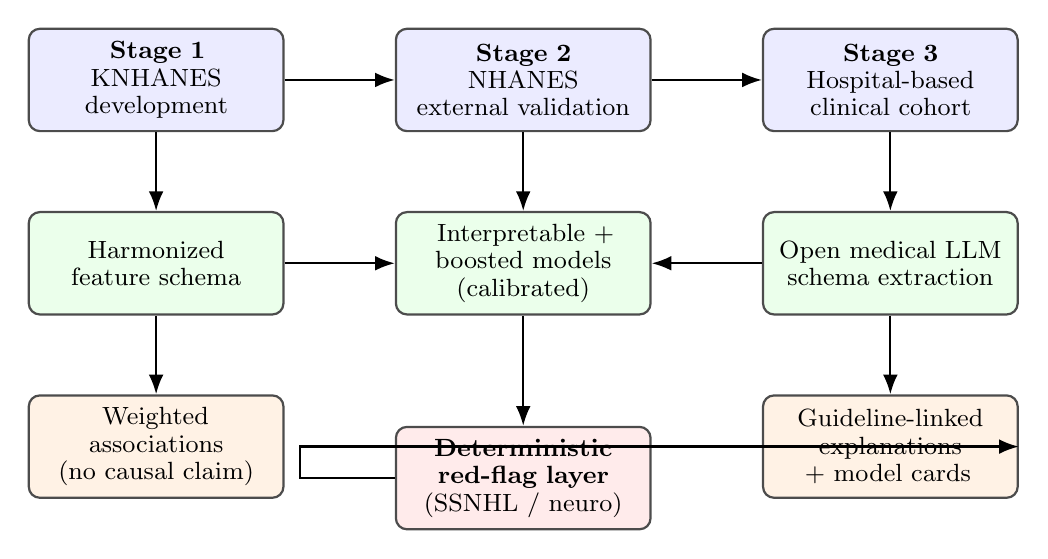
\begin{tikzpicture}[
  node distance=10mm and 14mm,
  box/.style={rectangle, rounded corners, draw=black!70, thick, align=center,
    text width=30mm, minimum height=13mm, font=\small\linespread{0.9}\selectfont},
  data/.style={box, fill=blue!8},
  ai/.style={box, fill=green!8},
  safe/.style={box, fill=red!8},
  outn/.style={box, fill=orange!10},
  arr/.style={-{Latex[length=2.5mm]}, thick}
]
\node[data] (knhanes) {\textbf{Stage 1}\\KNHANES\\development};
\node[data, right=of knhanes] (nhanes) {\textbf{Stage 2}\\NHANES\\external validation};
\node[data, right=of nhanes] (clinic) {\textbf{Stage 3}\\Hospital-based\\clinical cohort};

\node[ai, below=of knhanes] (harm) {Harmonized\\feature schema};
\node[ai, below=of nhanes] (model) {Interpretable +\\boosted models\\(calibrated)};
\node[ai, below=of clinic] (llm) {Open medical LLM\\schema extraction};

\node[safe, below=14mm of model] (redflag) {\textbf{Deterministic}\\\textbf{red-flag layer}\\(SSNHL / neuro)};

\node[outn, below=of harm] (assoc) {Weighted\\associations\\(no causal claim)};
\node[outn, below=of llm] (explain) {Guideline-linked\\explanations\\+ model cards};

\draw[arr] (knhanes) -- (nhanes);
\draw[arr] (nhanes) -- (clinic);
\draw[arr] (knhanes) -- (harm);
\draw[arr] (nhanes) -- (model);
\draw[arr] (clinic) -- (llm);
\draw[arr] (harm) -- (model);
\draw[arr] (llm) -- (model);
\draw[arr] (model) -- (redflag);
\draw[arr] (harm) -- (assoc);
\draw[arr] (llm) -- (explain);
\draw[arr] (redflag.west) -- ++(-1.2,0) |- (explain.east);
\end{tikzpicture}
\caption{STARS conceptual framework. Public survey data (blue) feed a harmonized schema and calibrated, interpretable models (green); an open medical language model performs schema-constrained extraction in the clinical extension. A deterministic red-flag safety layer (red) can override probabilistic output to force urgent referral, so a low predicted risk never suppresses time-critical SSNHL care. Outputs (orange) are associations and guideline-linked explanations, not diagnoses.}
\label{fig:framework}
\end{figure}

\begin{figure}[htbp]
\centering
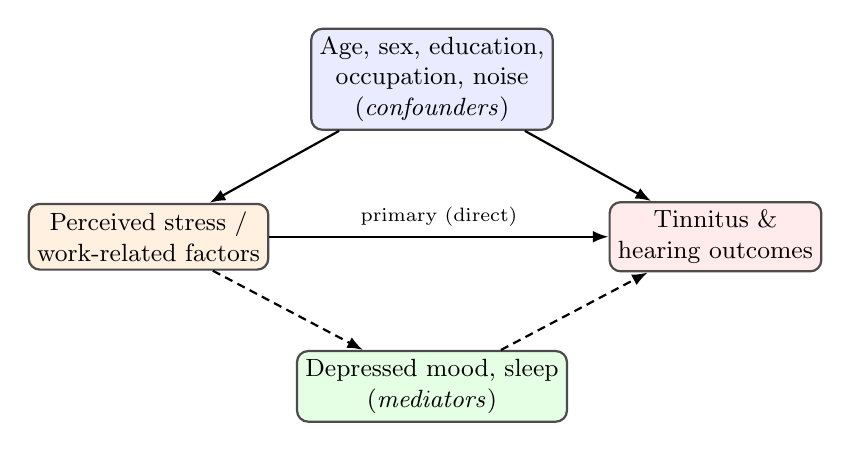
\begin{tikzpicture}[
  every node/.style={font=\small},
  var/.style={rectangle, rounded corners, draw=black!70, thick, align=center,
    inner sep=3pt, minimum height=8mm},
  conf/.style={var, fill=blue!8},
  expo/.style={var, fill=orange!12},
  med/.style={var, fill=green!10},
  outv/.style={var, fill=red!8},
  a/.style={-{Latex[length=2mm]}, thick},
  amed/.style={-{Latex[length=2mm]}, thick, densely dashed}
]
\node[expo] (stress) at (0,0) {Perceived stress /\\work-related factors};
\node[outv] (outc) at (7.2,0) {Tinnitus \&\\hearing outcomes};
\node[med] (dep) at (3.6,-1.9) {Depressed mood, sleep\\(\emph{mediators})};
\node[conf] (conf) at (3.6,2.0) {Age, sex, education,\\occupation, noise\\(\emph{confounders})};

\draw[a] (stress) -- node[above,font=\scriptsize]{primary (direct)} (outc);
\draw[amed] (stress) -- (dep);
\draw[amed] (dep) -- (outc);
\draw[a] (conf) -- (stress);
\draw[a] (conf) -- (outc);
\end{tikzpicture}
\caption{Assumed causal directed acyclic graph (DAG). The minimal sufficient adjustment set (blue confounders) is used in the \emph{primary} analysis. Depressed mood and sleep (green) are treated as \emph{mediators} of the stress$\rightarrow$outcome path (dashed); conditioning on them (extended model) is a mediator-adjusted, potentially overadjusted estimate reported separately. Restricting to employed adults can open a selection/collider path, so all-adult analysis is primary and employed-restricted analysis is secondary.}
\label{fig:dag}
\end{figure}

\begin{table}[htbp]
\centering
\caption{Selected public datasets for HEAR-WORK AI}
\label{tab:datasets}
\begin{tabular}{p{0.18\linewidth}p{0.26\linewidth}p{0.24\linewidth}p{0.22\linewidth}}
\toprule
Dataset & Role & Strengths & Main limitations \\
\midrule
KNHANES & Primary development dataset & Korean population relevance; audiometry in selected cycles; tinnitus and health variables; survey weights & Cross-sectional; stress variables may be perceived stress rather than validated occupational stress; raw data access procedures required \\
NHANES & External validation dataset & Public CDC files; audiometry and noise exposure in selected cycles; rich health covariates; geographic validation & U.S. population; cycle-specific hearing and tinnitus variables; complex survey design \\
OHHR / Zenodo audiology data & Secondary method testing & Audiology-specific measurements; useful for model benchmarking & May lack stress, occupation, or tinnitus variables \\
OpenNeuro tinnitus datasets & Optional neurophysiology substudy & Public neuroimaging or fNIRS data for tinnitus biomarkers & Not designed for occupational stress or longitudinal treatment outcomes \\
\bottomrule
\end{tabular}
\end{table}

\begin{table}[htbp]
\centering
\caption{Target harmonized variables and their availability in the primary public datasets. Availability is cycle-dependent; each derived variable records its source items and transformation in the version-controlled data dictionary.}
\label{tab:variables}
\small
\begin{tabular}{p{0.30\linewidth}p{0.14\linewidth}p{0.22\linewidth}p{0.22\linewidth}}
\toprule
Harmonized variable & Role & KNHANES & NHANES \\
\midrule
Pure-tone thresholds (per ear, per frequency) & Outcome & Selected cycles & Selected cycles \\
Tinnitus status / bother & Outcome & Selected cycles & Selected cycles \\
Self-reported hearing difficulty & Outcome (2\textsuperscript{nd}) & Yes & Yes \\
Hearing-aid use & Outcome (2\textsuperscript{nd}) & Selected cycles & Selected cycles \\
Perceived stress / depressed mood & Exposure & Yes & Yes \\
Occupation / employment status & Modifier & Yes & Yes \\
Occupational + recreational noise & Covariate & Selected cycles & Yes \\
Sleep duration & Covariate & Selected cycles & Selected cycles \\
Smoking, alcohol & Covariate & Yes & Yes \\
Cardiometabolic disease & Covariate & Yes & Yes \\
Age, sex, education & Covariate & Yes & Yes \\
Survey weight, stratum, PSU & Design & Yes & Yes \\
\bottomrule
\end{tabular}
\end{table}

\begin{table}[htbp]
\centering
\caption{Cross-national harmonization and measurement-comparability plan (excerpt). Exact cycle-specific variable codes and response categories are pinned in the repository data dictionary. Comparability governs use: \emph{low}-comparability variables are excluded from the common transportable model and entered only in country-specific extended models. ``Sel.\ cycles'' = present in selected cycles only.}
\label{tab:harmonization}
\scriptsize
\begin{tabular}{p{0.155\linewidth}p{0.145\linewidth}p{0.145\linewidth}p{0.175\linewidth}p{0.135\linewidth}p{0.085\linewidth}}
\toprule
Harmonized variable & KNHANES (source/cycle) & NHANES (source/cycle) & Original item (abridged) & Transformation rule & Compar. \\
\midrule
Tinnitus presence & Otologic Q, 2009--2012 & Audiometry Q (AUQ), sel.\ cycles & ``Ringing/noise in ears past 12 mo?'' & Any vs.\ none (binary) & High \\
Bothersome tinnitus & Otologic Q, 2009--2012 & AUQ bother item, sel.\ cycles & Annoyance / sleep / concentration & Bothersome vs.\ not & Medium \\
Pure-tone thresholds & Audiometry exam, 2010--2012 & Audiometry exam, sel.\ cycles & Air-conduction dB HL per freq. & Better/worse-ear PTA; per-ear & High \\
Perceived stress & Health Q (stress item) & DPQ / stress-related item & ``How much stress in daily life?'' & Collapse to high vs.\ low & \textbf{Low} \\
Depressed mood & PHQ-9 / mood item & PHQ-9 (DPQ) & Standardized depression items & Screen-positive vs.\ negative & Medium \\
Occupation / employment & Socioecon.\ Q & Occupation (OCQ) & Job category, employed y/n & Common category crosswalk & Medium \\
Occupational noise & Sel.\ cycles & Noise exposure (AUQ) & Loud-noise exposure, duration & Duration/intensity + binary & Medium \\
Sleep duration & Health Q & Sleep (SLQ) & Average hours of sleep & Continuous hours & Medium \\
Smoking / alcohol & Health Q & SMQ / ALQ & Current status, quantity & Standard categories & High \\
Age, sex, education & Demographics & Demographics (DEMO) & --- & Direct / crosswalk & High \\
Survey weight, stratum, PSU & Design vars & Design vars & --- & Kept for design-consistent SEs & High \\
\bottomrule
\end{tabular}
\end{table}

\begin{table}[htbp]
\centering
\caption{Intended-use specification for the two prediction models. Both are \emph{research risk-stratification} tools only; neither is a screening, diagnostic, or triage device. The specification is fixed before validation so that performance is judged against a declared purpose.}
\label{tab:intended}
\small
\begin{tabular}{p{0.24\linewidth}p{0.70\linewidth}}
\toprule
Dimension & Specification \\
\midrule
Purpose & Research risk stratification for cohort description and hypothesis generation; \emph{not} individual screening, diagnosis, triage, or treatment guidance. \\
Target user & Researchers/epidemiologists analyzing survey or, later, deidentified cohort data. \\
Prediction time & Cross-sectional (concurrent survey visit); no temporal/prognostic claim. \\
Target population & Adults 40--69 y in the fixed audiometry windows; not generalized beyond. \\
Inputs & Prespecified harmonized covariates (Table~\ref{tab:variables}); no free-text or image inputs in the public-data models. \\
Output / decision & Calibrated probability for research stratification; drives \emph{no} clinical action. \\
Cost of false positive & Low in research use; would be non-trivial if misused for screening (over-referral) --- such use is contraindicated. \\
Cost of false negative & Low in research use; dangerous if misused clinically (missed disease) --- such use is contraindicated. \\
Contraindicated uses & Individual diagnosis, treatment decisions, insurance/employment decisions, or any deployment without prospective clinical validation and regulatory review. \\
Safety interaction & The deterministic red-flag layer (Table~\ref{tab:redflag}) overrides model output for time-critical symptoms regardless of predicted probability. \\
\bottomrule
\end{tabular}
\end{table}

\begin{table}[htbp]
\centering
\caption{AI components and safety constraints}
\label{tab:ai}
\begin{tabular}{p{0.24\linewidth}p{0.34\linewidth}p{0.30\linewidth}}
\toprule
Component & Intended use & Safety constraint \\
\midrule
Survey harmonization & Map KNHANES/NHANES variables to common schema & Human-readable mapping file and version control \\
Statistical baseline & Estimate adjusted associations and transparent risk scores & Survey-aware methods; no causal claims from cross-sectional data \\
MedGemma or similar open medical LLM & Extract fixed fields from deidentified clinical notes in future cohorts & Clinician verification; no diagnosis or treatment recommendation \\
Retrieval-augmented explanation & Draft evidence-linked explanations for researchers and clinicians & Curated sources only; unsupported outputs flagged \\
Red-flag rule layer & Identify sudden hearing-loss or neurologic warning signs & Deterministic referral rules override probabilistic model \\
\bottomrule
\end{tabular}
\end{table}

\begin{table}[htbp]
\centering
\caption{Prespecified evaluation metrics (frozen before external validation). The right column shows \emph{synthetic-scaffold} values that verify pipeline wiring only: they are computed on randomly generated data, carry \textbf{no} epidemiological meaning, and must not be read as results. Real-data estimates replace them when KNHANES/NHANES files are supplied.}
\label{tab:metrics}
\small
\begin{tabular}{p{0.24\linewidth}p{0.46\linewidth}p{0.20\linewidth}}
\toprule
Dimension & Metric(s) & \textit{Synthetic scaffold (not a result)} \\
\midrule
Discrimination & AUROC, AUPRC (unweighted and survey-weighted) & Tinnitus: 0.64 / 0.49 \\
Calibration & Calibration-in-the-large and calibration slope, reported separately, before and after recalibration; Brier score; plots & Tinnitus Brier: 0.20 \\
Transportability & Common-support region; case-mix-standardized performance; reduced-common vs.\ country-specific model & Reported per target \\
Clinical utility & Decision-curve net benefit & Reported per target \\
Interpretability & SHAP importance (descriptive; caveated for correlated predictors) & Reported per target \\
Fairness & Subgroup AUROC \& calibration: sex, age, employment, noise, asymmetry, SES, race/ethnicity & Reported per subgroup \\
LLM extraction & Exact match; precision/recall/F1; omission; span agreement; temporal/laterality/onset/duration accuracy; doc-level match; run consistency; clinically significant error rate & Clinical extension \\
Safety layer & Sensitivity (95\% CI); specificity/over-referral; subgroup \& robustness (Table~\ref{tab:redflag}) & Target $\rightarrow$ 1.0 \\
\bottomrule
\end{tabular}
\end{table}

\begin{table}[htbp]
\centering
\caption{Prespecified evaluation plan for the deterministic red-flag (SSNHL/neurologic) safety layer. Sensitivity (red-flag recall) is the primary metric because a missed red flag is the costly error; but a perfect score on a finite test set does not guarantee zero real-world misses, and this limitation is stated explicitly.}
\label{tab:redflag}
\small
\begin{tabular}{p{0.28\linewidth}p{0.66\linewidth}}
\toprule
Evaluation element & Prespecification \\
\midrule
Vignette set & $\geq$200 vignettes; composition fixed: real deidentified clinical cases, expert-authored cases, and synthetic cases in a stated ratio (e.g., 40/30/30\%). \\
Reference labeling & Each vignette independently labeled by $\geq$2 otolaryngology/audiology experts; disagreements adjudicated. \\
Inter-rater agreement & Reported (Cohen's/Fleiss' $\kappa$) before adjudication. \\
Primary metric & Sensitivity (red-flag recall) with 95\% CI. \\
Secondary metrics & Specificity and over-referral rate with 95\% CIs. \\
Subgroup performance & By laterality (unilateral/bilateral), onset (acute/gradual), and vertigo/neurologic signs. \\
Robustness & Negation, ambiguous temporal expressions, and colloquial patient phrasing explicitly tested. \\
Error analysis & Every missed red flag audited and reported as a critical failure. \\
Stated limitation & Finite-set sensitivity of 1.0 is a target, not a guarantee of zero misses in deployment. \\
\bottomrule
\end{tabular}
\end{table}

\begin{thebibliography}{99}
\bibitem[Baigi et~al.(2011)]{baigi2011tinnitus} Baigi A, Oden A, Almlid-Larsen V, Barrenäs ML, Holgers KM. (2011). Tinnitus in the general population with a focus on noise and stress: A public health study. \textit{Ear and Hearing}, 32(6), 787--789. doi:10.1097/AUD.0b013e31822229bd
\bibitem[Chakrabarty et~al.(2024)]{chakrabarty2024depression} Chakrabarty S, et al. (2024). Contribution of tinnitus and hearing loss to depression: NHANES population data. \textit{Ear and Hearing}.
\bibitem[Chandrasekhar et~al.(2019)]{chandrasekhar2019ssnhl} Chandrasekhar SS, Tsai Do BS, Schwartz SR, et al. (2019). Clinical practice guideline: Sudden hearing loss (update). \textit{Otolaryngology--Head and Neck Surgery}, 161(1\_suppl), S1--S45. doi:10.1177/0194599819859885
\bibitem[Collins et~al.(2024)]{collins2024tripodai} Collins GS, Moons KGM, Dhiman P, et al. (2024). TRIPOD+AI statement: Updated guidance for reporting clinical prediction models that use regression or machine learning methods. \textit{BMJ}, 385, e078378. doi:10.1136/bmj-2023-078378
\bibitem[Google Research(2025)]{medgemma2025blog} Google Research. (2025). MedGemma: Open models for health AI development. \url{https://research.google/blog/medgemma-our-most-capable-open-models-for-health-ai-development/}
\bibitem[Google Health AI(2026)]{medgemma2026docs} Google Health AI Developer Foundations. (2026). MedGemma. \url{https://developers.google.com/health-ai-developer-foundations/medgemma}
\bibitem[Ha et~al.(2022)]{ha2022localization} Ha J, Kim H, Lee JH, Park HY. (2022). Sound localization in patients with a unilateral hearing aid: Discordance between the right and left ears. \textit{Laryngoscope Investigative Otolaryngology}, 7(2), 578--584. doi:10.1002/lio2.769
\bibitem[Hoffman et~al.(2020)]{hoffman2020noise} Hoffman HJ, et al. (2020). Noise exposure and hearing loss: Data from U.S. health surveys. CDC/NIOSH report.
\bibitem[Joo et~al.(2015)]{joo2015hrqol} Joo YH, Han K, Park KH. (2015). Association of hearing loss and tinnitus with health-related quality of life: The Korea National Health and Nutrition Examination Survey. \textit{PLoS ONE}, 10(6), e0131247.
\bibitem[Kim et~al.(2022)]{kim2022bppv} Kim H, Ha J, Lee JH, Jang JH, Park HY, Choung YH. (2022). Early management for traumatic benign paroxysmal positional vertigo in traumatically injured patients. \textit{Injury}, 53(1), 302--307. doi:10.1016/j.injury.2021.07.042
\bibitem[Kim et~al.(2021)]{kim2021ct} Kim H, Choo OS, Ha J, Jang JH, Park HY, Choung YH. (2021). A new CT parameter for predicting residual hearing preservation in cochlear implantation: The basal turn--facial ridge angle. \textit{Otology \& Neurotology}, 42(2), 204--211. doi:10.1097/MAO.0000000000002918
\bibitem[Mahboubi et~al.(2013)]{mahboubi2013noise} Mahboubi H, Zardouz S, Oliaei S, Pan D, Bazargan M, Djalilian HR. (2013). Noise-induced hearing threshold shift among U.S. adults and implications for noise-induced hearing loss. \textit{European Archives of Oto-Rhino-Laryngology}, 270, 461--467.
\bibitem[McCormack et~al.(2016)]{mccormack2016review} McCormack A, Edmondson-Jones M, Somerset S, Hall D. (2016). A systematic review of the reporting of tinnitus prevalence and severity. \textit{Hearing Research}, 337, 70--79. doi:10.1016/j.heares.2016.05.009
\bibitem[Park et~al.(2014)]{park2014tinnitus} Park KH, Lee SH, Koo JW, et al. (2014). Prevalence and associated factors of tinnitus: Data from the Korean National Health and Nutrition Examination Surveys 2009--2011. \textit{Journal of Epidemiology}, 24(5), 417--426.
\bibitem[Tunkel et~al.(2014)]{tunkel2014cpg} Tunkel DE, Bauer CA, Sun GH, et al. (2014). Clinical practice guideline: Tinnitus. \textit{Otolaryngology--Head and Neck Surgery}, 151(2\_suppl), S1--S40. doi:10.1177/0194599814545325
\bibitem[von Elm et~al.(2007)]{vonelm2007strobe} von Elm E, Altman DG, Egger M, Pocock SJ, Gøtzsche PC, Vandenbroucke JP. (2007). The Strengthening the Reporting of Observational Studies in Epidemiology (STROBE) statement. \textit{Annals of Internal Medicine}, 147(8), 573--577. doi:10.7326/0003-4819-147-8-200710160-00010
\bibitem[World Health Organization(2021)]{who2021world} World Health Organization. (2021). \textit{World Report on Hearing}. Geneva: WHO. \url{https://www.who.int/publications/i/item/9789240020481}
\end{thebibliography}

\end{document}
"
%   bibtex main ; then repeat the pdflatex line twice more.
% Upload paper/title_page.tex separately as the non-anonymized title page.
% NOTE: identity-revealing self-citations and in-text institution mentions are
% NOT auto-masked (removing them would damage the text) — see paper/README.md.
\newif\ifblind
\ifdefined\BLIND\blindtrue\else\blindfalse\fi
% ---------------------------------------------------------------------------

\title{STARS: A Pre-Analysis Protocol for Public-Data Studies of Perceived Stress, Work-Related Factors, Tinnitus, and Hearing Outcomes\\[2pt]\large With a Cross-National External-Validation Plan and a Deterministic Referral-Safety Layer}
\ifblind
\author{\normalsize\textit{[Author names and affiliations withheld for masked review]}}
\else
\author[1]{Geunsik Lim}
\author[2]{Hyun Jo}
\affil[1]{Sungkyunkwan University, Republic of Korea; \texttt{leemgs@g.skku.edu}}
\affil[2]{Ajou University School of Medicine, Republic of Korea; \texttt{joehyun@ajou.ac.kr}}
\fi
\date{Draft version 0.9: August 1, 2026}

\begin{document}
\maketitle
\thispagestyle{fancy}

\begin{center}
\small
\begin{tabular}{ll}
\textbf{Article type:} & Study Protocol / Pre-Analysis Plan with primary KNHANES + supporting NHANES results \\
\textbf{Target journal:} & \textit{American Journal of Audiology} (AJA) \\
\textbf{Running head:} & Perceived Stress, Tinnitus, and Hearing (Protocol) \\
\textbf{Reporting guidelines:} & STROBE; TRIPOD+AI; SPIRIT (clinical extension) \\
\textbf{Empirical findings:} & Primary real KNHANES results (Table~\ref{tab:results_knhanes}); supporting NHANES results (Table~\ref{tab:results}) \\
\textbf{Abstract:} & Structured, $\sim$320 words \\
\textbf{Body word count (target):} & $\sim$7{,}500 (excludes abstract, references, tables) \\
\textbf{Tables:} & 6 \qquad \textbf{Figures:} 2 \\
\ifblind\textbf{Open repository:} & [URL withheld for masked review] \\\else\textbf{Open repository:} & \url{https://github.com/leemgs/stars-audiology} \\\fi
\end{tabular}
\end{center}

\begin{abstract}
\noindent\textbf{Purpose:} This is a \emph{pre-analysis study protocol} for STARS (Stress, Tinnitus, and Audiometric Research Study), not an empirical report. It prespecifies public-data analyses of the associations among \emph{perceived stress and work-related factors}, tinnitus, and hearing outcomes in adults, together with a cross-national external-validation plan and a clinician-governed, safety-gated artificial-intelligence (AI) architecture. We deliberately avoid causal overclaiming: because the population surveys do not contain validated occupational-stress instruments, the exposure is labeled perceived stress and work-related factors---not measured occupational stress---and is treated as potentially \emph{associated} with tinnitus burden and hearing-related outcomes rather than as a proven cause of cochlear injury. We report the \emph{primary} perceived-stress analysis in KNHANES (which carries a general stress item) together with a \emph{supporting} analysis in NHANES.

\textbf{Method (prespecified):} The Korea National Health and Nutrition Examination Survey (KNHANES) is the development dataset and the U.S. National Health and Nutrition Examination Survey (NHANES) is the geographic external-validation dataset; we fix the survey cycles, age windows, audiometric frequencies, exclusions, and expected analytic sample sizes in advance. A causal directed acyclic graph (DAG) defines a minimal sufficient adjustment set and separates confounders from mediators (e.g., depressed mood, sleep), with primary analyses avoiding overadjustment and full-adult versus employed-restricted analyses addressing the healthy-worker effect. Endpoints (tinnitus presence, bothersome tinnitus, better- and worse-ear pure-tone average, and asymmetry) are modeled with survey-weighted regression; two \emph{research-only} risk-stratification models are evaluated with discrimination, calibration-in-the-large and calibration slope (before and after recalibration), decision-curve utility, common-support checks, and subgroup fairness (including socioeconomic status and race/ethnicity), reported per STROBE and TRIPOD+AI. A deterministic red-flag layer for sudden sensorineural hearing loss (SSNHL) overrides model output; its evaluation prespecifies vignette composition, dual otolaryngology/audiology labeling, inter-rater agreement, and sensitivity with confidence intervals. An open medical language model (e.g., MedGemma) is confined to schema-constrained extraction verified by clinicians.

\textbf{Contributions:} (1) a survey-weighted public-data framework that distinguishes stress--tinnitus from stress--audiometric-threshold associations without unsupported causal claims; (2) a prespecified KNHANES$\rightarrow$NHANES external-validation plan reporting calibration, recalibration, clinical utility, and subgroup fairness; (3) a clinically governed AI architecture in which schema-constrained extraction is clinician-verified and a deterministic red-flag layer overrides probabilistic predictions for time-critical hearing symptoms; and (4) an open, reproducible scaffold of harmonized variable mappings, executable code, model cards, safety tests, and a synthetic-data pathway.

\textbf{Primary results (KNHANES, adults 40--69, cycles 2010--2012):} Survey-weighted prevalence was 21.1\% (95\% CI 19.9--22.3) for tinnitus and 15.4\% (14.5--16.4) for better-ear hearing loss ($>$25 dB HL), with high perceived stress at 24.3\% (23.2--25.3). In the mutually adjusted, minimal-sufficient model (perceived stress, occupational noise, age, sex), high perceived stress was associated with \emph{tinnitus} (OR 1.42, 1.26--1.60, $p<0.001$) but only weakly and non-significantly with \emph{audiometric hearing loss} (OR 1.18, 0.99--1.41, $p=0.07$), which was instead dominated by occupational noise (OR 1.72, 1.44--2.06) and age (OR 1.13/year). This symptom-versus-threshold dissociation is exactly the prespecified pattern of hypothesis H1. \textbf{Supporting results (NHANES):} using a PHQ-9 distress proxy (a mediator, since NHANES lacks a stress item), the same dissociation held. All estimates are associations, not causal effects.

\textbf{Conclusions:} Registered public-data analyses can rigorously characterize associations and benchmark explainable, safety-gated AI, but prospective clinical cohorts remain necessary for treatment timing, recovery, and prognosis. STARS fixes the design, safety governance, and reproducible scaffold, and demonstrates the primary perceived-stress finding end-to-end on real KNHANES data, with NHANES as cross-national support.
\end{abstract}

\noindent\textbf{Keywords:} tinnitus; bothersome tinnitus; hearing loss; audiometry; perceived stress; work-related factors; sudden sensorineural hearing loss; KNHANES; NHANES; external validation; explainable AI; open medical language models; TRIPOD+AI; study protocol; reproducibility; audiology.

\section{Introduction}
Tinnitus and hearing loss are among the most common auditory health concerns
worldwide, affecting communication, sleep, mood, work participation, and quality
of life. More than 1.5 billion people live with some hearing loss, a number
projected to rise by 2050 \citep{who2021world}, and tinnitus affects an estimated
10--15\% of adults, a meaningful subset of whom experience bothersome tinnitus
\citep{tunkel2014cpg,mccormack2016review}. In employed middle-aged adults,
tinnitus frequently emerges alongside psychosocial stress, sleep disruption,
noise, and delayed help-seeking; because these factors are intertwined, simple
causal narratives are unreliable and can mislead patients and clinicians.

\subsection{Motivating observation and naming principle}
Consider an anonymized composite trajectory: a worker in their late 40s develops
unilateral tinnitus during heavy workload, which resolves over months; about a
year later the other ear develops sudden fullness and reduced audibility, but---
unaware of the narrow treatment window for sudden sensorineural hearing loss
(SSNHL)---the person delays care, and recovery is incomplete. Two clinically
actionable points follow: stress-associated tinnitus is common and often
self-limiting, but sudden or rapidly progressive hearing loss is an urgency in
which delayed care, not stress, drives irreversible impairment. Attributing acute
hearing symptoms to ``stress'' without assessment is hazardous. Accordingly, STARS
(Stress, Tinnitus, and Audiometric Research Study) adopts a strict naming
principle: because KNHANES and NHANES carry general perceived-stress and mood
items rather than validated job-strain instruments, we never call the exposure
measured ``occupational stress.'' It is labeled \emph{perceived stress}, with
\emph{work-related factors} (occupation, employment, and where available hours and
shift work) modeled as distinct covariates.

\subsection{A survey-weighted study reported against a prespecified plan}
This is a survey-weighted study whose \emph{primary} hypothesis test---the
perceived-stress analysis in KNHANES---is reported in full
(Section~\ref{sec:results}), with supporting NHANES analyses. To limit analyst
degrees of freedom, the design, variable definitions, cycles, adjustment sets, and
evaluation plan were fixed \emph{before} analysis, and committed code and outputs
make every value reproducible. Three further components---cross-national
validation, clinician-verified AI extraction, and a clinical extension---are
\emph{prospective} (design only) and kept subordinate to the empirical finding.

\subsection{Aims and hypotheses}
Aim~1 is the empirical contribution reported here; Aim~3 is developed \emph{with
results} in the companion SAFE-EAR paper, Aim~4's open pipeline accompanies this
article, and Aim~2 is prospective.
\begin{enumerate}[leftmargin=1.5em,itemsep=2pt]
\item \textbf{Association (development).} Estimate weighted associations between
perceived stress and (a) tinnitus and (b) audiometric hearing loss in KNHANES,
adjusting for noise and health covariates. \emph{H1: a positive stress--tinnitus
association persists after adjustment, while the association with audiometric
thresholds is weaker and may attenuate to non-significance after adjusting for
noise and age.}
\item \textbf{Transportability.} Test whether harmonized models developed in
KNHANES retain discrimination and calibration in NHANES. \emph{H2: discrimination
degrades modestly but calibration is restorable by recalibration.}
\item \textbf{Explainable, safe AI (companion paper).} Evaluate whether
schema-constrained extraction feeding a deterministic red-flag layer routes SSNHL
and neurologic warning signs to urgent referral. \emph{H3: near-complete red-flag
recall, bounded by extraction quality.} Developed with results in SAFE-EAR.
\item \textbf{Open, shared benefit.} Provide an openly licensed, reproducible
pipeline (code, data dictionary, model cards, prompts).
\end{enumerate}

\subsection{Contributions}
Primary: a survey-weighted, public-data result showing that perceived stress
dissociates the tinnitus \emph{symptom} from the audiometric \emph{threshold},
reported without unsupported causal claims and reproducible end-to-end. Secondary:
an open, reproducible scaffold (harmonized mappings, design-based estimators,
model cards, safety tests) that lets others regenerate every number and add local
cohorts. The remaining components---a prespecified KNHANES$\rightarrow$NHANES
external-validation plan and a clinically governed AI/referral-safety component in
which a deterministic red-flag layer overrides probabilistic predictions---are
prospective (design only); any prediction model is a research risk-stratification
tool, never a screening, diagnostic, or triage device.

\section{Related Work}
\subsection{Epidemiology and prior KNHANES work}
Tinnitus and hearing loss often coexist but relate heterogeneously. KNHANES
analyses have estimated Korean tinnitus prevalence and correlates
\citep{park2014tinnitus,joo2015hrqol}, and NHANES has enabled U.S. studies of
audiometry, occupational noise, tinnitus, and mental-health correlates
\citep{hoffman2017declining,chakrabarty2024depression,mahboubi2013noise}; reviews
emphasize heterogeneous case definitions and the need for harmonized variables
when pooling across surveys \citep{mccormack2016review}. Evidence linking
psychological stress to tinnitus is consistent but largely observational, with
residual confounding by noise, sleep, and cardiometabolic factors difficult to
exclude \citep{baigi2011tinnitus}. On the same KNHANES cycles, prior work has
examined tinnitus alongside distress---most closely \citet{lee2018tinnitus}, on
higher perceived stress and mood symptoms in premenopausal women with tinnitus.
STARS is therefore \emph{not} the first to link tinnitus with distress in KNHANES;
its contribution is methodological: (i) a \emph{prespecified, falsifiable} contrast
between the tinnitus \emph{symptom} and the audiometric \emph{threshold} (H1)
rather than a single tinnitus--distress association; (ii) an explicit DAG that
separates confounders from mediators, reporting both minimal-sufficient and
mediator-adjusted models; (iii) a cross-national directional-consistency check in
NHANES under a related distress construct; and (iv) a fully reproducible open
scaffold. The novelty is design discipline and reproducibility, not the mere
existence of a tinnitus--stress association.

\subsection{Beyond the pure-tone average}
Because real-world listening difficulty and tinnitus burden can persist when the
better-ear pure-tone average appears near-normal, STARS separates tinnitus
presence from bothersome tinnitus and analyzes worse-ear and high-frequency
thresholds and asymmetry, not better-ear PTA alone.

\subsection{Clinical pathways and reporting standards}
Practice guidelines frame the endpoints. The tinnitus guideline distinguishes
bothersome from non-bothersome tinnitus and prioritizes education,
cognitive-behavioral strategies, and sound therapy \citep{tunkel2014cpg}, while the
sudden-hearing-loss guideline defines a ``golden window''---prompt audiometric
confirmation and early corticosteroid therapy within roughly two weeks---so delayed
presentation is associated with worse outcomes \citep{chandrasekhar2019ssnhl}. This
is the clinical rationale for the deterministic red-flag referral-safety layer
developed in the companion SAFE-EAR paper. The observational analyses adhere to
STROBE \citep{vonelm2007strobe}; the prospective prediction and open-medical-LLM
components follow the TRIPOD+AI statement \citep{collins2024tripodai}.

\section{Public Dataset Selection}
Dataset selection was governed by four requirements for the primary association analyses: (i) survey-weighted population representativeness; (ii) objective pure-tone audiometry; (iii) tinnitus and/or hearing-difficulty items; and (iv) covariates for noise exposure, psychosocial stress, and general health. Only KNHANES and NHANES jointly satisfy all four at population scale. Supplementary Table~S1 summarizes the selection, and Supplementary Table~S2 maps target variables to each source.

\subsection{Primary Development Dataset: KNHANES}
KNHANES is selected as the primary development dataset because it is nationally representative for Korea and has previously supported tinnitus and hearing-loss analyses \citep{park2014tinnitus,joo2015hrqol}. Its advantages include Korean population relevance, complex-survey weights, pure-tone audiometry in applicable cycles (otologic examination cycles 2010--2012), tinnitus and hearing-difficulty questionnaire items in selected cycles, health and behavioral covariates, and psychosocial or stress-related self-report variables (e.g., perceived-stress and depressed-mood items). It also provides a realistic bridge to future Korean hospital cohorts, including the planned prospective clinical extension. Because item wording and audiometry availability differ across cycles, the analysis prespecifies a per-cycle codebook review and restricts pooling to cycles with comparable definitions.

The limitations are equally important. KNHANES is not a workplace cohort, and the audiometric analyses are cross-sectional. It can therefore evaluate \emph{associations} among perceived stress, work-related variables, tinnitus, and audiometric outcomes, but cannot by itself establish that occupational stress \emph{caused} tinnitus or hearing loss. Treatment timing and recovery after sudden hearing loss are not captured.

\subsection{External-Validation Dataset: NHANES}
NHANES is selected as the primary external-validation dataset because it provides openly downloadable U.S. public-use files, pure-tone audiometry and tympanometry in selected cycles (2011--2012, 2015--2016, 2017--2018), occupational and recreational noise-exposure items, tinnitus and hearing questionnaires in selected cycles, and extensive demographic and health covariates. NHANES enables testing whether feature definitions and risk models derived from KNHANES retain discrimination and calibration across population, language, health-system, and occupational contexts. As with KNHANES, complex-survey weights, strata, and primary sampling units must be honored, and cycle-specific age eligibility for the audiometry module must be respected.

\subsection{Prospective Clinical Extension (Hospital-Based Cohort)}
A prospective otolaryngology/audiology cohort is specified to address what public cross-sectional data cannot---treatment timing, SSNHL recovery, longitudinal tinnitus burden, and rehabilitation---and to supply deidentified audiograms and clinical narratives for the companion clinical validation and safety evaluations (Supplementary Methods~S2). Raw clinical data are not redistributed; only derived, deidentified, or synthetic artifacts are shared, subject to IRB approval.

\section{Methods (Prespecified)}
This pre-analysis protocol is reported following STROBE for the observational analyses \citep{vonelm2007strobe} and TRIPOD+AI for the prediction models \citep{collins2024tripodai}; the prospective clinical extension will follow SPIRIT. A completed reporting checklist accompanies the repository. All design choices below are fixed prior to any real-data analysis.

\subsection{Study Design}
The work has three stages, summarized in the conceptual framework of Figure~\ref{fig:framework}. \textbf{Stage~1} analyzes KNHANES as the primary public-data development cohort (association estimation and research-model development). \textbf{Stage~2} evaluates cross-national transportability in NHANES (geographic external validation). \textbf{Stage~3} prepares a prospective clinical extension at Ajou University Hospital for clinical external validation, treatment-timing analysis in SSNHL, and evaluation of the AI extraction and safety components. Stages~1--2 use only deidentified public-use files; Stage~3 proceeds only under IRB approval.

\subsection{Fixed Datasets, Cycles, and Eligibility}
To eliminate analyst degrees of freedom, the survey cycles, files, ages, frequencies, and exclusions are fixed in advance (Table~\ref{tab:datasets}). \textbf{KNHANES:} the otologic-examination cycles carrying pure-tone audiometry and tinnitus items (KNHANES IV--V, 2009--2012) form the primary development window; cycles are pooled only after confirming identical item wording and audiometry protocols. \textbf{NHANES:} the audiometry-module cycles 2011--2012, 2015--2016, and 2017--March~2020 form the external-validation window. For both, eligible records are adults aged 40--69~years (the band jointly covered by the audiometry modules and our target of mid-to-late-career workers), with valid examination weights and a non-missing value for the outcome under analysis. Pure-tone thresholds are analyzed at 0.5, 1, 2, 3, 4, 6, and 8~kHz per ear; conductive patterns are flagged and, where tympanometry/air--bone data permit, excluded in a sensitivity analysis. We prespecify expected raw and analytic sample sizes per window (reported in the repository data dictionary) and the exact set of predictors available in \emph{both} surveys; any predictor available in only one survey is excluded from the common transportable model and used only in country-specific extended models.

\subsection{Exposure: Perceived Stress and Work-Related Factors}
Consistent with the naming principle (Introduction), the primary exposure is \emph{perceived stress}, operationalized from each survey's general stress/psychological-distress item, and \emph{work-related factors} (occupation category, employment status, and---where a cycle provides them---working hours and shift work) are modeled as separate covariates or effect modifiers, never as a proxy for validated job strain. Because item wording, response categories, and cultural response styles differ across surveys, Table~\ref{tab:harmonization} records, for every exposure and covariate, the original question, response scale, harmonization rule, and a measurement-comparability rating (high/medium/low). Variables rated \emph{low} comparability (typically the stress and some psychosocial items) are (a) excluded from the common transportable model, (b) entered only in country-specific models, and (c) examined in a formal measurement-invariance check (configural/metric where a latent construct is defined). We do not pool a variable across countries unless at least metric-level comparability is plausible.

\subsection{Causal Structure and Adjustment Sets}
Figure~\ref{fig:dag} presents the directed acyclic graph (DAG) encoding our assumptions. Age, sex, education, occupation/employment, and noise exposure are treated as confounders of the perceived-stress$\rightarrow$outcome relationships and constitute the \textbf{minimal sufficient adjustment set} for the primary analysis. Depressed mood and sleep are treated as \emph{potential mediators} of the stress$\rightarrow$tinnitus path (and possibly colliders when conditioning opens non-causal paths); conditioning on them can constitute overadjustment. Accordingly:
\begin{itemize}[leftmargin=1.4em,itemsep=1pt]
\item \textbf{Primary model} adjusts for the minimal sufficient set only (age, sex, education, occupation/employment, noise).
\item \textbf{Extended model} additionally includes depressed mood and sleep, reported separately and interpreted as a mediator-adjusted (not confounder-adjusted) estimate.
\item \textbf{Mediation analysis} decomposes total, direct, and indirect (through depressed mood/sleep) associations under stated assumptions, as an exploratory addendum.
\item \textbf{Collider check} enumerates conditioning sets that could induce collider bias and excludes them from the primary specification.
\end{itemize}
Because restricting to employed participants can induce a healthy-worker effect (and a selection collider), the primary population is \emph{all eligible adults}, with an \emph{employed-restricted} analysis reported as a prespecified secondary contrast rather than the main result.

\subsection{Outcomes}
Endpoints are defined a priori and separated:
\begin{itemize}[leftmargin=1.4em,itemsep=1pt]
\item \textbf{Tinnitus presence} (any tinnitus in the past 12 months) and \textbf{bothersome tinnitus} (tinnitus causing annoyance/sleep or concentration difficulty) are modeled as \emph{distinct} endpoints, since their determinants differ.
\item \textbf{Hearing loss} is quantified by the speech-frequency pure-tone average (PTA$_{0.5,1,2,4}$) for \emph{both the better ear and the worse ear}, plus a \textbf{per-ear} (ear-level, mixed-effects) analysis, because a better-ear summary can mask the unilateral/asymmetric presentations most relevant to SSNHL. The primary threshold is PTA $>25$~dB HL (the WHO grade-1 cutoff \citep{who2021world}); $>20$~dB HL and high-frequency PTA$_{3,4,6}$ are prespecified sensitivity definitions, with the 25~dB HL choice justified as the established clinical cutpoint.
\item \textbf{Asymmetric hearing loss} is defined as an interaural difference $\geq$15~dB at $\geq$2 adjacent frequencies, consistent with asymmetry criteria used in sudden/asymmetric hearing-loss guidance \citep{chandrasekhar2019ssnhl}.
\item \textbf{Secondary:} self-reported hearing difficulty, hearing-aid use, and quality-of-life correlates.
\end{itemize}
\textbf{Noise exposure} is coded, where cycles permit, not merely as a binary but with duration, intensity/source (occupational, recreational, firearm), and hearing-protection use, so residual confounding by noise is minimized.

\subsection{Statistical Analysis}
All public-data analyses use survey-aware methods (Taylor-linearization variance estimation honoring weights, strata, and PSUs). Descriptive analyses estimate weighted prevalence with 95\% confidence intervals. Association analyses use weighted logistic, ordinal, or linear regression by outcome type. The \textbf{primary specification adjusts for the minimal sufficient set}; the extended (mediator-adjusted) model is secondary. Results are reported as associations (odds ratios or mean differences) with 95\% CIs, explicitly not as causal effects. Multiplicity is handled by prespecifying primary hypotheses (Introduction) and controlling the false-discovery rate across secondary contrasts.

\paragraph{Missing data.} Missingness is described by variable and mechanism. Primary analyses use multiple imputation by chained equations under a missing-at-random assumption (design variables in the imputation model), pooled by Rubin's rules; complete-case analysis is a sensitivity check. In external validation, records missing a common predictor are handled by the same prespecified rule in both surveys.

\paragraph{Sample size and precision.} Sample sizes are fixed, so we frame precision rather than post-hoc power: with several thousand audiometry participants per window, weighted prevalence is estimable to within a few percentage points and moderate associations (OR~$\approx$~1.3--1.5) are detectable at conventional error rates. Exact expected analytic $N$ per window is fixed in the repository before analysis.

\subsection{Research-Only Prediction Models and Intended Use}
Two targets---tinnitus presence and audiometric hearing loss---are developed as \emph{research risk-stratification models}, not screening, diagnostic, or triage devices. Their intended use, target user, prediction time, inputs, decision, and the costs of false positives/negatives and contraindicated uses are specified in Table~\ref{tab:intended}. We first fit transparent survey-weighted logistic baselines with prespecified predictors, then gradient-boosted trees as a comparator; the simpler model is preferred unless the complex model yields a clinically meaningful, calibrated improvement. Development uses KNHANES with repeated stratified cross-validation and optimism correction. All targets, predictors, and metrics are frozen before external validation (Table~\ref{tab:metrics}). SHAP values are reported for interpretability, with the explicit caveat that SHAP does not guarantee causal or even stable attributions when predictors are correlated; importance is interpreted descriptively, not causally.

\subsection{External Validation Across Survey Designs}
Transporting a KNHANES model to NHANES confronts differences in weighting, population prevalence, age range, category coding, and health-system context. We therefore prespecify:
\begin{itemize}[leftmargin=1.4em,itemsep=1pt]
\item \textbf{Unweighted vs.\ weighted performance} reported separately---unweighted for individual-level prediction, survey-weighted for population-level performance.
\item \textbf{Calibration-in-the-large and calibration slope reported separately}, before and after recalibration (intercept-only, then intercept+slope update of the frozen model).
\item \textbf{Common-support analysis} restricting comparison to the overlapping covariate region of the two surveys.
\item \textbf{Case-mix standardization} to distinguish genuine model transportability from case-mix differences in prevalence/age.
\item \textbf{A reduced common model} (predictors available and comparable in both surveys) versus \textbf{country-specific extended models}, so that limited measurement invariance does not masquerade as poor transportability.
\end{itemize}

\paragraph{Fairness and subgroup evaluation.} Discrimination and calibration are reported within prespecified subgroups: sex, age band, employment status, noise-exposure status, unilateral/asymmetric hearing, \emph{socioeconomic status} (education/income), and \emph{race/ethnicity} (NHANES, where collected). Subgroup calibration and error gaps are first-class results, not afterthoughts.

\subsection{Sensitivity Analyses}
Prespecified sensitivity analyses test alternative hearing-loss definitions (25 vs.\ 20~dB HL; high-frequency PTA; worse-ear and per-ear), age restrictions, exclusion of conductive patterns when tympanometry permits, alternative stress operationalizations, mediator- vs.\ confounder-treatment of depressed mood/sleep, all-adult vs.\ employed-restricted populations, and stratification by noise exposure, sex, and asymmetry.

\subsection{Ethics and Governance}
Stages~1--2 use publicly available, deidentified survey data and do not constitute human-subjects research requiring new consent; KNHANES and NHANES were approved by their respective review boards, and their use follows each provider's data-use terms. The Stage-3 clinical extension will obtain IRB approval at Ajou University Hospital, with a data-management plan covering deidentification, access control, and secondary-use consent. No identifiable patient data are placed in the public repository; only derived, deidentified, or synthetic artifacts are shared.

\section{Open AI System and Research Acceleration}
\label{sec:ai}
\subsection{Motivation}
A major barrier to audiology AI is the scarcity of harmonized, reusable clinical features. StressEar-AI addresses this by publishing a transparent feature schema, reproducible public-data code, and a clinician-verification protocol. This supports a broadly shared-benefit research model: investigators can reuse the pipeline, add local cohorts, and compare models without exposing identifiable patient data.

\subsection{Model Roles and Prohibitions}
The AI system has four restricted roles: (1) it harmonizes variable names and labels across public datasets; (2) it trains transparent baseline models for association and calibrated risk stratification; (3) in the clinical extension, an open medical language model (e.g., MedGemma) extracts structured fields from deidentified notes using a fixed JSON schema; and (4) it drafts explanations that cite only approved study documents or clinical guidelines. The system is explicitly prohibited from diagnosing an individual patient, assigning a definitive etiology, recommending or dosing steroids, or delaying urgent referral. These prohibitions are enforced in code and documented in a model card.

\subsection{Deterministic Red-Flag Safety Layer}
Before any probabilistic model output is surfaced, a deterministic rule layer screens for red flags derived from the SSNHL and tinnitus guidelines \citep{chandrasekhar2019ssnhl,tunkel2014cpg}: sudden or rapidly progressive hearing loss (especially unilateral), aural fullness with a discrete onset, single-sided tinnitus with asymmetry, vertigo, or focal neurologic signs. Any trigger overrides the model and returns an ``urgent audiology/otolaryngology referral'' message. The layer is evaluated primarily on recall (missed red flags are the costly error); its rules, versions, and test cases are unit-tested in the repository. This operationalizes the ``golden-window'' lesson from the motivating vignette: the framework must never let a probabilistic ``low-risk, likely stress'' estimate suppress timely referral.

\subsection{Schema-Constrained Extraction and Governance}
LLM extraction is constrained to a fixed schema with typed fields and controlled vocabularies; free-text generation is disallowed for structured outputs. Each extracted field is accompanied by a source span and a confidence flag, and every field is subject to clinician verification before entering analysis. Prompts, schema versions, model weights/version, temperature, and random seeds are logged. Extraction quality is reported as human-verified field accuracy, unsupported-output (hallucination) rate, and a clinician review of any potentially harmful output.

\subsection{Robustness and Trustworthiness}
Trustworthiness is pursued through eight design choices: (1) public-data baselines; (2) country-level external validation; (3) survey-weighted epidemiology; (4) interpretable models before complex models; (5) locked feature and outcome definitions; (6) clinician review of LLM-extracted variables; (7) subgroup calibration and error analysis; and (8) full run provenance (dataset versions, variable mappings, hyperparameters, prompts, seeds). Reproducibility is supported by pinned dependencies and deterministic seeds.

\subsection{Open-Science Contribution}
The repository includes executable analysis templates, a data dictionary, model cards, prompt templates, a red-flag test suite, and a completed reporting checklist. Because KNHANES files cannot be redistributed without official access procedures, the code specifies directory expectations and variable-mapping scripts rather than repackaging raw data. NHANES download helpers retrieve public files directly from CDC endpoints where available. A synthetic-data generator lets others exercise the full pipeline end-to-end without any restricted data, lowering the barrier to reuse and review.

\section{Results}\label{sec:results}
We report the \emph{primary} perceived-stress analyses in the KNHANES development
cohort, then the \emph{supporting} NHANES analyses. KNHANES is the primary test
because, unlike NHANES, it carries a general perceived-stress item (the NHANES
PHQ-9 proxy is a DAG \emph{mediator}). All estimates are design-based
(survey-weighted, Taylor-linearized) associations, not causal effects, and every
value below is reproduced by the committed \texttt{outputs/knhanes\_results.json}
and \texttt{nhanes\_results.json}.

\subsection{Primary results (KNHANES, adults 40--69)}
Pooling the otologic-examination cycles 2010--2012 (KNHANES V; analytic domain
$n=10{,}467$; complete-case models retained 9{,}142--9{,}532 by outcome),
survey-weighted prevalence was 21.1\% (95\% CI 19.9--22.3) for any tinnitus, 7.0\%
(6.3--7.7) for bothersome tinnitus, 15.4\% (14.5--16.4) for better-ear
speech-frequency hearing loss ($>$25 dB HL), and 24.3\% (23.2--25.3) for high
perceived stress.
\IfFileExists{tables/table_results_knhanes.tex}{\begin{table}[htbp]
\centering
\caption{\textbf{Real KNHANES results} (Korean adults 40--69). Primary development cohort with the perceived-stress exposure. Prevalence is design-based (survey-weighted, Taylor-linearized); associations are mutually adjusted design-based odds ratios and are \emph{not} causal. Generated by \texttt{code/src/knhanes\_analysis.py}. $^{*}p<0.05$, $^{**}p<0.01$, $^{***}p<0.001$.}
\label{tab:results_knhanes}
\small
\begin{tabular}{lcc}
\toprule
 & Tinnitus & Hearing loss ($>$25 dB HL) \\
\midrule
Prevalence (95\% CI) & 21.1\% (19.9--22.3) & 15.4\% (14.5--16.4) \\
\midrule
\multicolumn{3}{l}{\emph{Adjusted associations, OR (95\% CI)}} \\
\quad Perceived stress (high) & 1.42 (1.26--1.60)*** & 1.18 (0.99--1.41) \\
\quad Occupational noise & 1.37 (1.15--1.63)*** & 1.72 (1.44--2.06)*** \\
\quad Age (per year) & 1.03 (1.02--1.04)*** & 1.13 (1.12--1.14)*** \\
\quad Female sex & 1.08 (0.96--1.22) & 0.47 (0.40--0.55)*** \\
\bottomrule
\end{tabular}
\end{table}
}{}

\paragraph{Primary association (H1).} In the minimal-sufficient model (perceived
stress, occupational noise, age, sex), high perceived stress was associated with
\emph{tinnitus} (OR 1.42, 1.26--1.60) but only weakly and non-significantly with
\emph{better-ear hearing loss} (OR 1.18, 0.99--1.41), where occupational noise (OR
1.72, 1.44--2.06) and age (OR 1.13 per year) dominated. This is the prespecified
symptom-versus-threshold dissociation (H1): perceived stress tracks the tinnitus
\emph{symptom} ($p<0.001$) but attenuates against the audiometric \emph{threshold}
($p=0.07$) once occupational noise and age are accounted for.

\paragraph{Sensitivity analyses.} The stress--tinnitus association survived
adjustment for the mediator depressed mood (OR 1.29, 1.13--1.47) and for
audiometric hearing loss itself (OR 1.44, 1.27--1.64), so it is not an artifact of
under-adjustment for the strongest tinnitus correlate
(Table~\ref{tab:results_knhanes_extended}). It persisted for \emph{non-bothersome}
tinnitus versus none (OR 1.24, 1.05--1.45) and was strongest for bothersome
tinnitus (OR 1.79, 1.46--2.21); across seven secondary contrasts we control the
false-discovery rate (Benjamini--Hochberg), and these remain significant
($q<0.02$). The dissociation is \emph{relative, not absolute}: perceived stress
was weakly associated with the \emph{worse-ear} threshold (OR 1.15, 1.00--1.31;
does not survive FDR, $q\approx0.07$) but not with the high-frequency definition
(OR 1.07, 0.93--1.23). Because the KNHANES examination provides air-conduction
thresholds and tympanometry but not bone conduction, we excluded middle-ear
pathology using normal bilateral tympanometry: the stress--threshold association
then \emph{strengthened} to significance (OR 1.29, 1.07--1.55) while the tinnitus
association was essentially unchanged (OR 1.42, 1.25--1.62), indicating the
full-sample null was partly a conductive-contamination artifact and that the
contrast is one of \emph{degree}.
\IfFileExists{tables/table_extended_knhanes.tex}{\begin{table}[htbp]
\centering
\caption{\textbf{Extended and sensitivity models (KNHANES, adults 40--69).}
Perceived-stress odds ratio (95\% CI) across prespecified specifications,
isolating the robustness of the primary exposure. Rows add the mediator
(depressed mood) or audiometric hearing loss to the minimal-sufficient set
(perceived stress, occupational noise, age, sex), and vary the hearing-loss
outcome definition (better-ear, worse-ear, high-frequency). All are design-based
associations, not causal effects; mediator-adjusted rows are interpreted as
mediator- (not confounder-) adjusted. Generated by
\texttt{code/src/knhanes\_analysis.py}. Cells marked \emph{[pending data run]}
populate automatically when the pipeline is executed on the KDCA-approved
microdata with \texttt{-{}-latex-extended}. $^{*}p<0.05$, $^{**}p<0.01$,
$^{***}p<0.001$.}
\label{tab:results_knhanes_extended}
\small
\begin{tabular}{lcc}
\toprule
Model specification & Perceived stress, OR (95\% CI) & $N$ \\
\midrule
Tinnitus --- minimal-sufficient (primary) & 1.42 (1.26--1.60)*** & 9504 \\
\quad + depressed mood (mediator-adjusted) & \textit{[pending data run]} & -- \\
\quad + audiometric hearing loss & \textit{[pending data run]} & -- \\
Hearing loss, better ear --- minimal-sufficient & 1.18 (0.99--1.41) & 9176 \\
\quad + depressed mood (mediator-adjusted) & \textit{[pending data run]} & -- \\
Hearing loss, worse ear --- minimal-sufficient & \textit{[pending data run]} & -- \\
Hearing loss, high-freq (3/4/6\,kHz) --- minimal-sufficient & \textit{[pending data run]} & -- \\
Bothersome tinnitus --- minimal-sufficient & \textit{[pending data run]} & -- \\
Non-bothersome tinnitus vs none (reverse-causation sensitivity) & \textit{[pending data run]} & -- \\
\bottomrule
\end{tabular}
\end{table}
}{}

The employed-restricted (healthy-worker) contrast, the KNHANES$\rightarrow$NHANES
external validation (H2), and subgroup fairness are prospective components that
follow the prespecified plan (Methods; Supplementary Methods~S1) and carry no
results here; the open-LLM extraction and referral-safety layer are developed,
with results, in the companion SAFE-EAR paper.

\subsection{Supporting results (NHANES): directional consistency}
For U.S. adults aged 40--69 (pooling 2011--2012, 2015--2016, 2017--2018;
Table~\ref{tab:results}), survey-weighted prevalence was 28.5\% (26.5--30.4) for
any tinnitus, 12.0\% (10.4--13.6) for better-ear hearing loss, and 8.4\% (7.5--9.4)
for a positive PHQ-9 screen. In mutually adjusted design-based models,
\emph{tinnitus} was associated with occupational noise (OR 1.59, 1.32--1.92),
depressed mood (OR 1.61, 1.23--2.11), and female sex (OR 1.61, 1.35--1.91) but not
age; \emph{hearing loss} was dominated by age (OR 1.11 per year, 1.09--1.13) and
depressed mood (OR 2.29, 1.56--3.35), inversely by female sex (OR 0.42,
0.29--0.61), and only weakly by noise (OR 1.22, 0.94--1.58). Because the PHQ-9
proxy is a DAG mediator and NHANES lacks the perceived-stress exposure, these
mediator-level associations reproduce the symptom-versus-threshold pattern in a
different population but do not substitute for the primary KNHANES analysis.
\IfFileExists{tables/table_results.tex}{\begin{table}[htbp]
\centering
\caption{Real NHANES survey-weighted results (adults 40--69). Estimates are design-based (Taylor-linearized); associations are odds ratios from design-weighted logistic regression and are not causal. Generated by \texttt{code/src/nhanes\_analysis.py}.}
\label{tab:results}
\small
\begin{tabular}{lll}
\toprule
Quantity & Estimate (95\% CI) & $N$ \\
\midrule
Tinnitus prevalence & 28.5\% (26.5--30.4) & 5354 \\
Hearing loss ($>$25 dB HL) prevalence & 12.0\% (10.4--13.6) & 4808 \\
Depression (PHQ-9$\geq$10) prevalence & 8.4\% (7.5--9.4) & 7293 \\
Tinnitus: OR depressed mood & 1.61 (1.23--2.11) & 4603 \\
Tinnitus: OR occupational noise & 1.59 (1.32--1.92) & 4603 \\
Hearing loss: OR depressed mood & 2.29 (1.56--3.35) & 4463 \\
Hearing loss: OR occupational noise & 1.22 (0.94--1.58) & 4463 \\
\bottomrule
\end{tabular}
\end{table}
}{}

\section{Discussion}
This AJA-targeted framework makes three deliberate commitments. First, it selects KNHANES as the primary public dataset because it is Korean, population-based, and relevant to the intended clinical setting, with NHANES for cross-national external validation. Second, it reframes AI as a reproducible research accelerator rather than a diagnostic authority, bounded by a deterministic safety layer. Third, it operationalizes reproducibility and shared benefit through fully open code, a data dictionary, model cards, and a synthetic-data path that lets anyone run the pipeline without restricted data.

\subsection{Interpretation}
The expected scientific contribution is \emph{not} a claim that workplace stress directly damages hearing. Rather, StressEar-AI quantifies whether stress-related measures are consistently associated with tinnitus, hearing difficulty, and audiometric outcomes after accounting for noise exposure and health covariates. We anticipate a robust stress--tinnitus association and a weaker, noise-confounded stress--threshold association (H1). This asymmetry, if confirmed, has a clear clinical reading: stress may amplify tinnitus perception and burden more than it shifts cochlear thresholds, which aligns with tinnitus being partly a central, attention-modulated phenomenon.

\subsection{Clinical contribution and the treatment window}
The clinical contribution is an audiology-centered pathway that separates screening, referral, treatment, and rehabilitation. The framework's most consequential clinical stance is procedural rather than statistical: because SSNHL is a time-critical emergency \citep{chandrasekhar2019ssnhl}, the system is engineered so that a low predicted risk can never suppress urgent referral. The motivating vignette---resolved unilateral stress-associated tinnitus followed a year later by a delayed-care sudden loss in the other ear---illustrates precisely the failure mode the red-flag layer exists to prevent. Public data can identify population patterns and high-risk profiles; the Ajou University Hospital extension can then test treatment timing, SSNHL recovery, speech-in-noise outcomes, hearing-aid rehabilitation, and tinnitus burden longitudinally.

\subsection{Comparison with prior work}
Unlike single-country prevalence studies \citep{park2014tinnitus,joo2015hrqol}, StressEar-AI prespecifies cross-national transportability testing and reports calibration and decision-curve utility, not discrimination alone. Unlike opaque clinical-AI demonstrations, it locks feature and outcome definitions before external validation, publishes model cards, and evaluates subgroup fairness as a primary result. This positions the framework as a reusable methodological baseline rather than a one-off result.

\subsection{Limitations}
Several limitations remain and temper interpretation. Stress measurement differs across datasets and may not capture validated occupational-stress constructs; we therefore label the exposure ``perceived stress'' when appropriate. Cross-sectional audiometry cannot establish temporal order, so no causal claim is made. Audiometry availability and item wording vary across survey cycles, constraining pooling. Tinnitus definitions and severity scales differ across sources. Public datasets lack detailed treatment timing, which only the prospective cohort can supply. Complex-survey design must be honored to avoid biased inference. Finally, open medical language models require local validation, privacy review, and clinical governance before any deployment; their outputs are confined here to research feature extraction and guideline-linked explanation, never to autonomous clinical decisions.

\subsection{Future directions}
Future work includes: adding longitudinal occupational cohorts to strengthen temporality; a neurophysiological substudy of tinnitus subtypes using open OpenNeuro/EEG datasets; audiogram-digitization to unlock legacy paper audiograms for retrospective analysis; and community extension of the harmonization schema to additional national health surveys, advancing a globally shared, reproducible evidence base.

\section{Conclusion}
HEAR-WORK AI provides a public-data-first, clinically grounded, and openly reproducible framework for studying tinnitus, hearing loss, and stress-related exposures in employed adults. KNHANES is the preferred development dataset, NHANES the preferred public external-validation dataset, and open medical AI models accelerate feature extraction and explanation only under schema constraints, a deterministic red-flag safety layer, and strict human verification. By prespecifying aims, honoring complex-survey design, reporting calibration and fairness, and releasing code, model cards, and a synthetic-data path, the framework improves reproducibility, robustness, and global usefulness while avoiding unsupported causal claims. Public data can establish associations and benchmark methods; the prospective clinical extension is required to study treatment timing and recovery---above all, to protect the narrow window in which sudden hearing loss is treatable.

\section*{Declarations}
\ifblind
\textbf{Author Contributions (CRediT):} \emph{[Withheld for masked review; provided on the separate title page.]}

\textbf{Corresponding Author:} \emph{[Withheld for masked review; provided on the separate title page.]}
\else
\textbf{Author Contributions (CRediT):} \emph{Geunsik Lim}---Conceptualization, Methodology, Software, Formal analysis, Data curation, Writing (original draft), Visualization. \emph{Hyun Jo}---Clinical methodology (audiology/otolaryngology), Validation, Supervision of the planned clinical extension, Writing (review \& editing). Both authors read and approved this draft.

\textbf{Corresponding Author:} Geunsik Lim, Sungkyunkwan University, Republic of Korea. Email: \texttt{leemgs@g.skku.edu}.
\fi

\textbf{Funding:} No external funding was received for this pre-analysis framework. Any funding for the prospective clinical extension will be disclosed at that stage.

\textbf{Ethics Approval:} Stages~1--2 use publicly available, fully deidentified survey microdata (KNHANES, NHANES) under each provider's data-use terms and do not constitute new human-subjects research. The Stage-3 clinical extension will obtain institutional review board approval at Ajou University Hospital before any data collection.

\textbf{Reporting Guidelines:} The observational analyses follow STROBE \citep{vonelm2007strobe}; the prediction models follow TRIPOD+AI \citep{collins2024tripodai}; the clinical extension will follow SPIRIT. A completed checklist is provided in the repository.

\textbf{Protocol Status and Registration:} This is a pre-analysis study protocol whose prespecified primary KNHANES perceived-stress analyses are now reported (Section~\ref{sec:results}), with NHANES as supporting cross-national evidence; the external-validation, AI-extraction, and clinical-extension components remain prospective. The prespecified analysis plan (cycles, variables, adjustment sets, endpoints, and metrics) is time-stamped in the versioned repository.

\textbf{Data Availability:} KNHANES data are available from the Korea Disease Control and Prevention Agency subject to official access procedures; NHANES public-use files are available from the U.S.\ CDC. The repository provides code, configuration, variable-mapping templates, and a synthetic-data generator, but does not redistribute restricted raw data.

\textbf{Code Availability:} All analysis code, configuration, model cards, prompt templates, and the reporting checklist are openly available \ifblind at \emph{[repository URL withheld for masked review]}\else at \url{https://github.com/leemgs/stars-audiology}\fi{} under an open-source license.

\textbf{AI-Use Disclosure:} Generative AI tools assisted in drafting and structuring this manuscript and the code scaffold; the authors reviewed and are responsible for all content. In the proposed study, open medical language models will be used only for research feature extraction and guideline-linked explanation from deidentified text, always with clinician verification before analysis and never for autonomous clinical decisions.

\textbf{Conflicts of Interest:} The authors declare no competing interests.

\begin{figure}[htbp]
\centering
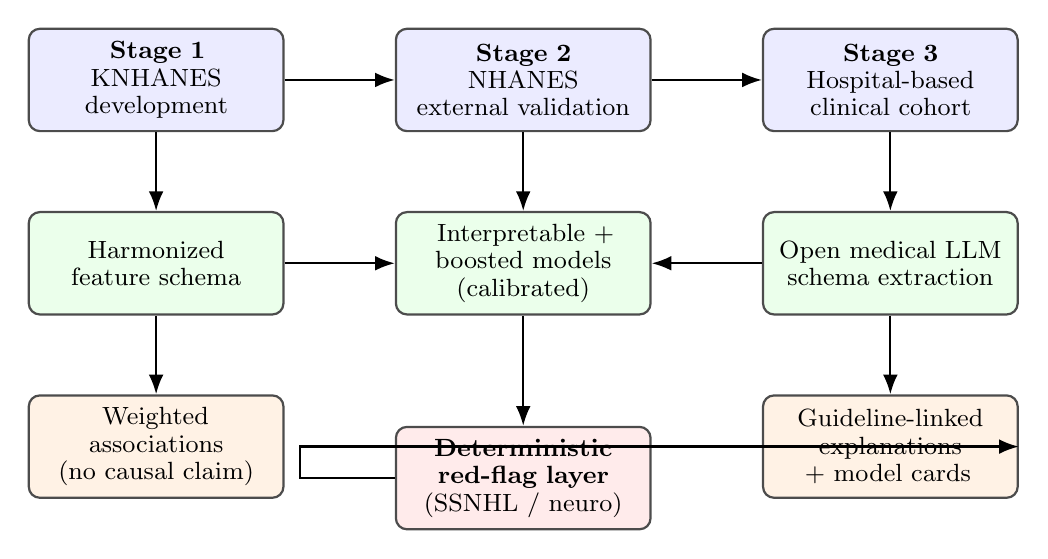
\begin{tikzpicture}[
  node distance=10mm and 14mm,
  box/.style={rectangle, rounded corners, draw=black!70, thick, align=center,
    text width=30mm, minimum height=13mm, font=\small\linespread{0.9}\selectfont},
  data/.style={box, fill=blue!8},
  ai/.style={box, fill=green!8},
  safe/.style={box, fill=red!8},
  outn/.style={box, fill=orange!10},
  arr/.style={-{Latex[length=2.5mm]}, thick}
]
\node[data] (knhanes) {\textbf{Stage 1}\\KNHANES\\development};
\node[data, right=of knhanes] (nhanes) {\textbf{Stage 2}\\NHANES\\external validation};
\node[data, right=of nhanes] (clinic) {\textbf{Stage 3}\\Hospital-based\\clinical cohort};

\node[ai, below=of knhanes] (harm) {Harmonized\\feature schema};
\node[ai, below=of nhanes] (model) {Interpretable +\\boosted models\\(calibrated)};
\node[ai, below=of clinic] (llm) {Open medical LLM\\schema extraction};

\node[safe, below=14mm of model] (redflag) {\textbf{Deterministic}\\\textbf{red-flag layer}\\(SSNHL / neuro)};

\node[outn, below=of harm] (assoc) {Weighted\\associations\\(no causal claim)};
\node[outn, below=of llm] (explain) {Guideline-linked\\explanations\\+ model cards};

\draw[arr] (knhanes) -- (nhanes);
\draw[arr] (nhanes) -- (clinic);
\draw[arr] (knhanes) -- (harm);
\draw[arr] (nhanes) -- (model);
\draw[arr] (clinic) -- (llm);
\draw[arr] (harm) -- (model);
\draw[arr] (llm) -- (model);
\draw[arr] (model) -- (redflag);
\draw[arr] (harm) -- (assoc);
\draw[arr] (llm) -- (explain);
\draw[arr] (redflag.west) -- ++(-1.2,0) |- (explain.east);
\end{tikzpicture}
\caption{STARS conceptual framework. Public survey data (blue) feed a harmonized schema and calibrated, interpretable models (green); an open medical language model performs schema-constrained extraction in the clinical extension. A deterministic red-flag safety layer (red) can override probabilistic output to force urgent referral, so a low predicted risk never suppresses time-critical SSNHL care. Outputs (orange) are associations and guideline-linked explanations, not diagnoses.}
\label{fig:framework}
\end{figure}

\begin{figure}[htbp]
\centering
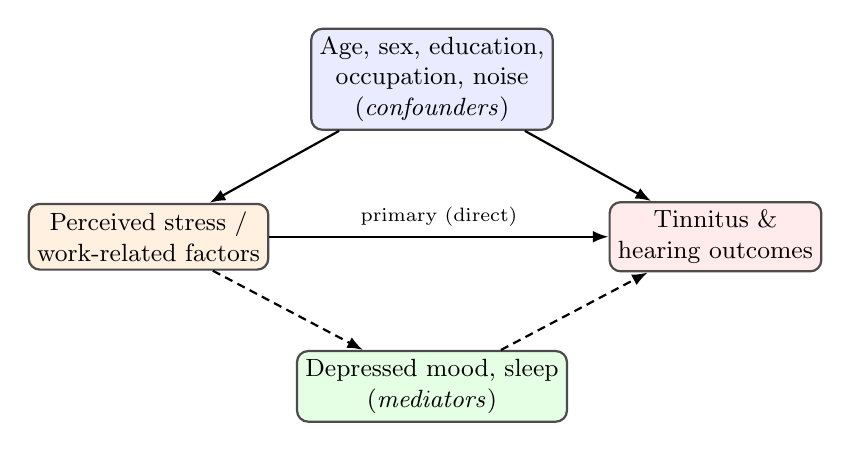
\begin{tikzpicture}[
  every node/.style={font=\small},
  var/.style={rectangle, rounded corners, draw=black!70, thick, align=center,
    inner sep=3pt, minimum height=8mm},
  conf/.style={var, fill=blue!8},
  expo/.style={var, fill=orange!12},
  med/.style={var, fill=green!10},
  outv/.style={var, fill=red!8},
  a/.style={-{Latex[length=2mm]}, thick},
  amed/.style={-{Latex[length=2mm]}, thick, densely dashed}
]
\node[expo] (stress) at (0,0) {Perceived stress /\\work-related factors};
\node[outv] (outc) at (7.2,0) {Tinnitus \&\\hearing outcomes};
\node[med] (dep) at (3.6,-1.9) {Depressed mood, sleep\\(\emph{mediators})};
\node[conf] (conf) at (3.6,2.0) {Age, sex, education,\\occupation, noise\\(\emph{confounders})};

\draw[a] (stress) -- node[above,font=\scriptsize]{primary (direct)} (outc);
\draw[amed] (stress) -- (dep);
\draw[amed] (dep) -- (outc);
\draw[a] (conf) -- (stress);
\draw[a] (conf) -- (outc);
\end{tikzpicture}
\caption{Assumed causal directed acyclic graph (DAG). The minimal sufficient adjustment set (blue confounders) is used in the \emph{primary} analysis. Depressed mood and sleep (green) are treated as \emph{mediators} of the stress$\rightarrow$outcome path (dashed); conditioning on them (extended model) is a mediator-adjusted, potentially overadjusted estimate reported separately. Restricting to employed adults can open a selection/collider path, so all-adult analysis is primary and employed-restricted analysis is secondary.}
\label{fig:dag}
\end{figure}

\begin{table}[htbp]
\centering
\caption{Selected public datasets for HEAR-WORK AI}
\label{tab:datasets}
\begin{tabular}{p{0.18\linewidth}p{0.26\linewidth}p{0.24\linewidth}p{0.22\linewidth}}
\toprule
Dataset & Role & Strengths & Main limitations \\
\midrule
KNHANES & Primary development dataset & Korean population relevance; audiometry in selected cycles; tinnitus and health variables; survey weights & Cross-sectional; stress variables may be perceived stress rather than validated occupational stress; raw data access procedures required \\
NHANES & External validation dataset & Public CDC files; audiometry and noise exposure in selected cycles; rich health covariates; geographic validation & U.S. population; cycle-specific hearing and tinnitus variables; complex survey design \\
OHHR / Zenodo audiology data & Secondary method testing & Audiology-specific measurements; useful for model benchmarking & May lack stress, occupation, or tinnitus variables \\
OpenNeuro tinnitus datasets & Optional neurophysiology substudy & Public neuroimaging or fNIRS data for tinnitus biomarkers & Not designed for occupational stress or longitudinal treatment outcomes \\
\bottomrule
\end{tabular}
\end{table}

\begin{table}[htbp]
\centering
\caption{Target harmonized variables and their availability in the primary public datasets. Availability is cycle-dependent; each derived variable records its source items and transformation in the version-controlled data dictionary.}
\label{tab:variables}
\small
\begin{tabular}{p{0.30\linewidth}p{0.14\linewidth}p{0.22\linewidth}p{0.22\linewidth}}
\toprule
Harmonized variable & Role & KNHANES & NHANES \\
\midrule
Pure-tone thresholds (per ear, per frequency) & Outcome & Selected cycles & Selected cycles \\
Tinnitus status / bother & Outcome & Selected cycles & Selected cycles \\
Self-reported hearing difficulty & Outcome (2\textsuperscript{nd}) & Yes & Yes \\
Hearing-aid use & Outcome (2\textsuperscript{nd}) & Selected cycles & Selected cycles \\
Perceived stress / depressed mood & Exposure & Yes & Yes \\
Occupation / employment status & Modifier & Yes & Yes \\
Occupational + recreational noise & Covariate & Selected cycles & Yes \\
Sleep duration & Covariate & Selected cycles & Selected cycles \\
Smoking, alcohol & Covariate & Yes & Yes \\
Cardiometabolic disease & Covariate & Yes & Yes \\
Age, sex, education & Covariate & Yes & Yes \\
Survey weight, stratum, PSU & Design & Yes & Yes \\
\bottomrule
\end{tabular}
\end{table}

\begin{table}[htbp]
\centering
\caption{Cross-national harmonization and measurement-comparability plan (excerpt). Exact cycle-specific variable codes and response categories are pinned in the repository data dictionary. Comparability governs use: \emph{low}-comparability variables are excluded from the common transportable model and entered only in country-specific extended models. ``Sel.\ cycles'' = present in selected cycles only.}
\label{tab:harmonization}
\scriptsize
\begin{tabular}{p{0.155\linewidth}p{0.145\linewidth}p{0.145\linewidth}p{0.175\linewidth}p{0.135\linewidth}p{0.085\linewidth}}
\toprule
Harmonized variable & KNHANES (source/cycle) & NHANES (source/cycle) & Original item (abridged) & Transformation rule & Compar. \\
\midrule
Tinnitus presence & Otologic Q, 2009--2012 & Audiometry Q (AUQ), sel.\ cycles & ``Ringing/noise in ears past 12 mo?'' & Any vs.\ none (binary) & High \\
Bothersome tinnitus & Otologic Q, 2009--2012 & AUQ bother item, sel.\ cycles & Annoyance / sleep / concentration & Bothersome vs.\ not & Medium \\
Pure-tone thresholds & Audiometry exam, 2010--2012 & Audiometry exam, sel.\ cycles & Air-conduction dB HL per freq. & Better/worse-ear PTA; per-ear & High \\
Perceived stress & Health Q (stress item) & DPQ / stress-related item & ``How much stress in daily life?'' & Collapse to high vs.\ low & \textbf{Low} \\
Depressed mood & PHQ-9 / mood item & PHQ-9 (DPQ) & Standardized depression items & Screen-positive vs.\ negative & Medium \\
Occupation / employment & Socioecon.\ Q & Occupation (OCQ) & Job category, employed y/n & Common category crosswalk & Medium \\
Occupational noise & Sel.\ cycles & Noise exposure (AUQ) & Loud-noise exposure, duration & Duration/intensity + binary & Medium \\
Sleep duration & Health Q & Sleep (SLQ) & Average hours of sleep & Continuous hours & Medium \\
Smoking / alcohol & Health Q & SMQ / ALQ & Current status, quantity & Standard categories & High \\
Age, sex, education & Demographics & Demographics (DEMO) & --- & Direct / crosswalk & High \\
Survey weight, stratum, PSU & Design vars & Design vars & --- & Kept for design-consistent SEs & High \\
\bottomrule
\end{tabular}
\end{table}

\begin{table}[htbp]
\centering
\caption{Intended-use specification for the two prediction models. Both are \emph{research risk-stratification} tools only; neither is a screening, diagnostic, or triage device. The specification is fixed before validation so that performance is judged against a declared purpose.}
\label{tab:intended}
\small
\begin{tabular}{p{0.24\linewidth}p{0.70\linewidth}}
\toprule
Dimension & Specification \\
\midrule
Purpose & Research risk stratification for cohort description and hypothesis generation; \emph{not} individual screening, diagnosis, triage, or treatment guidance. \\
Target user & Researchers/epidemiologists analyzing survey or, later, deidentified cohort data. \\
Prediction time & Cross-sectional (concurrent survey visit); no temporal/prognostic claim. \\
Target population & Adults 40--69 y in the fixed audiometry windows; not generalized beyond. \\
Inputs & Prespecified harmonized covariates (Table~\ref{tab:variables}); no free-text or image inputs in the public-data models. \\
Output / decision & Calibrated probability for research stratification; drives \emph{no} clinical action. \\
Cost of false positive & Low in research use; would be non-trivial if misused for screening (over-referral) --- such use is contraindicated. \\
Cost of false negative & Low in research use; dangerous if misused clinically (missed disease) --- such use is contraindicated. \\
Contraindicated uses & Individual diagnosis, treatment decisions, insurance/employment decisions, or any deployment without prospective clinical validation and regulatory review. \\
Safety interaction & The deterministic red-flag layer (Table~\ref{tab:redflag}) overrides model output for time-critical symptoms regardless of predicted probability. \\
\bottomrule
\end{tabular}
\end{table}

\begin{table}[htbp]
\centering
\caption{AI components and safety constraints}
\label{tab:ai}
\begin{tabular}{p{0.24\linewidth}p{0.34\linewidth}p{0.30\linewidth}}
\toprule
Component & Intended use & Safety constraint \\
\midrule
Survey harmonization & Map KNHANES/NHANES variables to common schema & Human-readable mapping file and version control \\
Statistical baseline & Estimate adjusted associations and transparent risk scores & Survey-aware methods; no causal claims from cross-sectional data \\
MedGemma or similar open medical LLM & Extract fixed fields from deidentified clinical notes in future cohorts & Clinician verification; no diagnosis or treatment recommendation \\
Retrieval-augmented explanation & Draft evidence-linked explanations for researchers and clinicians & Curated sources only; unsupported outputs flagged \\
Red-flag rule layer & Identify sudden hearing-loss or neurologic warning signs & Deterministic referral rules override probabilistic model \\
\bottomrule
\end{tabular}
\end{table}

\begin{table}[htbp]
\centering
\caption{Prespecified evaluation metrics (frozen before external validation). The right column shows \emph{synthetic-scaffold} values that verify pipeline wiring only: they are computed on randomly generated data, carry \textbf{no} epidemiological meaning, and must not be read as results. Real-data estimates replace them when KNHANES/NHANES files are supplied.}
\label{tab:metrics}
\small
\begin{tabular}{p{0.24\linewidth}p{0.46\linewidth}p{0.20\linewidth}}
\toprule
Dimension & Metric(s) & \textit{Synthetic scaffold (not a result)} \\
\midrule
Discrimination & AUROC, AUPRC (unweighted and survey-weighted) & Tinnitus: 0.64 / 0.49 \\
Calibration & Calibration-in-the-large and calibration slope, reported separately, before and after recalibration; Brier score; plots & Tinnitus Brier: 0.20 \\
Transportability & Common-support region; case-mix-standardized performance; reduced-common vs.\ country-specific model & Reported per target \\
Clinical utility & Decision-curve net benefit & Reported per target \\
Interpretability & SHAP importance (descriptive; caveated for correlated predictors) & Reported per target \\
Fairness & Subgroup AUROC \& calibration: sex, age, employment, noise, asymmetry, SES, race/ethnicity & Reported per subgroup \\
LLM extraction & Exact match; precision/recall/F1; omission; span agreement; temporal/laterality/onset/duration accuracy; doc-level match; run consistency; clinically significant error rate & Clinical extension \\
Safety layer & Sensitivity (95\% CI); specificity/over-referral; subgroup \& robustness (Table~\ref{tab:redflag}) & Target $\rightarrow$ 1.0 \\
\bottomrule
\end{tabular}
\end{table}

\begin{table}[htbp]
\centering
\caption{Prespecified evaluation plan for the deterministic red-flag (SSNHL/neurologic) safety layer. Sensitivity (red-flag recall) is the primary metric because a missed red flag is the costly error; but a perfect score on a finite test set does not guarantee zero real-world misses, and this limitation is stated explicitly.}
\label{tab:redflag}
\small
\begin{tabular}{p{0.28\linewidth}p{0.66\linewidth}}
\toprule
Evaluation element & Prespecification \\
\midrule
Vignette set & $\geq$200 vignettes; composition fixed: real deidentified clinical cases, expert-authored cases, and synthetic cases in a stated ratio (e.g., 40/30/30\%). \\
Reference labeling & Each vignette independently labeled by $\geq$2 otolaryngology/audiology experts; disagreements adjudicated. \\
Inter-rater agreement & Reported (Cohen's/Fleiss' $\kappa$) before adjudication. \\
Primary metric & Sensitivity (red-flag recall) with 95\% CI. \\
Secondary metrics & Specificity and over-referral rate with 95\% CIs. \\
Subgroup performance & By laterality (unilateral/bilateral), onset (acute/gradual), and vertigo/neurologic signs. \\
Robustness & Negation, ambiguous temporal expressions, and colloquial patient phrasing explicitly tested. \\
Error analysis & Every missed red flag audited and reported as a critical failure. \\
Stated limitation & Finite-set sensitivity of 1.0 is a target, not a guarantee of zero misses in deployment. \\
\bottomrule
\end{tabular}
\end{table}

\begin{thebibliography}{99}
\bibitem[Baigi et~al.(2011)]{baigi2011tinnitus} Baigi A, Oden A, Almlid-Larsen V, Barrenäs ML, Holgers KM. (2011). Tinnitus in the general population with a focus on noise and stress: A public health study. \textit{Ear and Hearing}, 32(6), 787--789. doi:10.1097/AUD.0b013e31822229bd
\bibitem[Chakrabarty et~al.(2024)]{chakrabarty2024depression} Chakrabarty S, et al. (2024). Contribution of tinnitus and hearing loss to depression: NHANES population data. \textit{Ear and Hearing}.
\bibitem[Chandrasekhar et~al.(2019)]{chandrasekhar2019ssnhl} Chandrasekhar SS, Tsai Do BS, Schwartz SR, et al. (2019). Clinical practice guideline: Sudden hearing loss (update). \textit{Otolaryngology--Head and Neck Surgery}, 161(1\_suppl), S1--S45. doi:10.1177/0194599819859885
\bibitem[Collins et~al.(2024)]{collins2024tripodai} Collins GS, Moons KGM, Dhiman P, et al. (2024). TRIPOD+AI statement: Updated guidance for reporting clinical prediction models that use regression or machine learning methods. \textit{BMJ}, 385, e078378. doi:10.1136/bmj-2023-078378
\bibitem[Google Research(2025)]{medgemma2025blog} Google Research. (2025). MedGemma: Open models for health AI development. \url{https://research.google/blog/medgemma-our-most-capable-open-models-for-health-ai-development/}
\bibitem[Google Health AI(2026)]{medgemma2026docs} Google Health AI Developer Foundations. (2026). MedGemma. \url{https://developers.google.com/health-ai-developer-foundations/medgemma}
\bibitem[Ha et~al.(2022)]{ha2022localization} Ha J, Kim H, Lee JH, Park HY. (2022). Sound localization in patients with a unilateral hearing aid: Discordance between the right and left ears. \textit{Laryngoscope Investigative Otolaryngology}, 7(2), 578--584. doi:10.1002/lio2.769
\bibitem[Hoffman et~al.(2020)]{hoffman2020noise} Hoffman HJ, et al. (2020). Noise exposure and hearing loss: Data from U.S. health surveys. CDC/NIOSH report.
\bibitem[Joo et~al.(2015)]{joo2015hrqol} Joo YH, Han K, Park KH. (2015). Association of hearing loss and tinnitus with health-related quality of life: The Korea National Health and Nutrition Examination Survey. \textit{PLoS ONE}, 10(6), e0131247.
\bibitem[Kim et~al.(2022)]{kim2022bppv} Kim H, Ha J, Lee JH, Jang JH, Park HY, Choung YH. (2022). Early management for traumatic benign paroxysmal positional vertigo in traumatically injured patients. \textit{Injury}, 53(1), 302--307. doi:10.1016/j.injury.2021.07.042
\bibitem[Kim et~al.(2021)]{kim2021ct} Kim H, Choo OS, Ha J, Jang JH, Park HY, Choung YH. (2021). A new CT parameter for predicting residual hearing preservation in cochlear implantation: The basal turn--facial ridge angle. \textit{Otology \& Neurotology}, 42(2), 204--211. doi:10.1097/MAO.0000000000002918
\bibitem[Mahboubi et~al.(2013)]{mahboubi2013noise} Mahboubi H, Zardouz S, Oliaei S, Pan D, Bazargan M, Djalilian HR. (2013). Noise-induced hearing threshold shift among U.S. adults and implications for noise-induced hearing loss. \textit{European Archives of Oto-Rhino-Laryngology}, 270, 461--467.
\bibitem[McCormack et~al.(2016)]{mccormack2016review} McCormack A, Edmondson-Jones M, Somerset S, Hall D. (2016). A systematic review of the reporting of tinnitus prevalence and severity. \textit{Hearing Research}, 337, 70--79. doi:10.1016/j.heares.2016.05.009
\bibitem[Park et~al.(2014)]{park2014tinnitus} Park KH, Lee SH, Koo JW, et al. (2014). Prevalence and associated factors of tinnitus: Data from the Korean National Health and Nutrition Examination Surveys 2009--2011. \textit{Journal of Epidemiology}, 24(5), 417--426.
\bibitem[Tunkel et~al.(2014)]{tunkel2014cpg} Tunkel DE, Bauer CA, Sun GH, et al. (2014). Clinical practice guideline: Tinnitus. \textit{Otolaryngology--Head and Neck Surgery}, 151(2\_suppl), S1--S40. doi:10.1177/0194599814545325
\bibitem[von Elm et~al.(2007)]{vonelm2007strobe} von Elm E, Altman DG, Egger M, Pocock SJ, Gøtzsche PC, Vandenbroucke JP. (2007). The Strengthening the Reporting of Observational Studies in Epidemiology (STROBE) statement. \textit{Annals of Internal Medicine}, 147(8), 573--577. doi:10.7326/0003-4819-147-8-200710160-00010
\bibitem[World Health Organization(2021)]{who2021world} World Health Organization. (2021). \textit{World Report on Hearing}. Geneva: WHO. \url{https://www.who.int/publications/i/item/9789240020481}
\end{thebibliography}

\end{document}
"
%   bibtex main ; then repeat the pdflatex line twice more.
% Upload paper/title_page.tex separately as the non-anonymized title page.
% NOTE: identity-revealing self-citations and in-text institution mentions are
% NOT auto-masked (removing them would damage the text) — see paper/README.md.
\newif\ifblind
\ifdefined\BLIND\blindtrue\else\blindfalse\fi
% ---------------------------------------------------------------------------

\title{STARS: A Pre-Analysis Protocol for Public-Data Studies of Perceived Stress, Work-Related Factors, Tinnitus, and Hearing Outcomes\\[2pt]\large With a Cross-National External-Validation Plan and a Deterministic Referral-Safety Layer}
\ifblind
\author{\normalsize\textit{[Author names and affiliations withheld for masked review]}}
\else
\author[1]{Geunsik Lim}
\author[2]{Hyun Jo}
\affil[1]{Sungkyunkwan University, Republic of Korea; \texttt{leemgs@g.skku.edu}}
\affil[2]{Ajou University School of Medicine, Republic of Korea; \texttt{joehyun@ajou.ac.kr}}
\fi
\date{Draft version 0.9: August 1, 2026}

\begin{document}
\maketitle
\thispagestyle{fancy}

\begin{center}
\small
\begin{tabular}{ll}
\textbf{Article type:} & Study Protocol / Pre-Analysis Plan with primary KNHANES + supporting NHANES results \\
\textbf{Target journal:} & \textit{American Journal of Audiology} (AJA) \\
\textbf{Running head:} & Perceived Stress, Tinnitus, and Hearing (Protocol) \\
\textbf{Reporting guidelines:} & STROBE; TRIPOD+AI; SPIRIT (clinical extension) \\
\textbf{Empirical findings:} & Primary real KNHANES results (Table~\ref{tab:results_knhanes}); supporting NHANES results (Table~\ref{tab:results}) \\
\textbf{Abstract:} & Structured, $\sim$320 words \\
\textbf{Body word count (target):} & $\sim$7{,}500 (excludes abstract, references, tables) \\
\textbf{Tables:} & 6 \qquad \textbf{Figures:} 2 \\
\ifblind\textbf{Open repository:} & [URL withheld for masked review] \\\else\textbf{Open repository:} & \url{https://github.com/leemgs/stars-audiology} \\\fi
\end{tabular}
\end{center}

\begin{abstract}
\noindent\textbf{Purpose:} This is a \emph{pre-analysis study protocol} for STARS (Stress, Tinnitus, and Audiometric Research Study), not an empirical report. It prespecifies public-data analyses of the associations among \emph{perceived stress and work-related factors}, tinnitus, and hearing outcomes in adults, together with a cross-national external-validation plan and a clinician-governed, safety-gated artificial-intelligence (AI) architecture. We deliberately avoid causal overclaiming: because the population surveys do not contain validated occupational-stress instruments, the exposure is labeled perceived stress and work-related factors---not measured occupational stress---and is treated as potentially \emph{associated} with tinnitus burden and hearing-related outcomes rather than as a proven cause of cochlear injury. We report the \emph{primary} perceived-stress analysis in KNHANES (which carries a general stress item) together with a \emph{supporting} analysis in NHANES.

\textbf{Method (prespecified):} The Korea National Health and Nutrition Examination Survey (KNHANES) is the development dataset and the U.S. National Health and Nutrition Examination Survey (NHANES) is the geographic external-validation dataset; we fix the survey cycles, age windows, audiometric frequencies, exclusions, and expected analytic sample sizes in advance. A causal directed acyclic graph (DAG) defines a minimal sufficient adjustment set and separates confounders from mediators (e.g., depressed mood, sleep), with primary analyses avoiding overadjustment and full-adult versus employed-restricted analyses addressing the healthy-worker effect. Endpoints (tinnitus presence, bothersome tinnitus, better- and worse-ear pure-tone average, and asymmetry) are modeled with survey-weighted regression; two \emph{research-only} risk-stratification models are evaluated with discrimination, calibration-in-the-large and calibration slope (before and after recalibration), decision-curve utility, common-support checks, and subgroup fairness (including socioeconomic status and race/ethnicity), reported per STROBE and TRIPOD+AI. A deterministic red-flag layer for sudden sensorineural hearing loss (SSNHL) overrides model output; its evaluation prespecifies vignette composition, dual otolaryngology/audiology labeling, inter-rater agreement, and sensitivity with confidence intervals. An open medical language model (e.g., MedGemma) is confined to schema-constrained extraction verified by clinicians.

\textbf{Contributions:} (1) a survey-weighted public-data framework that distinguishes stress--tinnitus from stress--audiometric-threshold associations without unsupported causal claims; (2) a prespecified KNHANES$\rightarrow$NHANES external-validation plan reporting calibration, recalibration, clinical utility, and subgroup fairness; (3) a clinically governed AI architecture in which schema-constrained extraction is clinician-verified and a deterministic red-flag layer overrides probabilistic predictions for time-critical hearing symptoms; and (4) an open, reproducible scaffold of harmonized variable mappings, executable code, model cards, safety tests, and a synthetic-data pathway.

\textbf{Primary results (KNHANES, adults 40--69, cycles 2010--2012):} Survey-weighted prevalence was 21.1\% (95\% CI 19.9--22.3) for tinnitus and 15.4\% (14.5--16.4) for better-ear hearing loss ($>$25 dB HL), with high perceived stress at 24.3\% (23.2--25.3). In the mutually adjusted, minimal-sufficient model (perceived stress, occupational noise, age, sex), high perceived stress was associated with \emph{tinnitus} (OR 1.42, 1.26--1.60, $p<0.001$) but only weakly and non-significantly with \emph{audiometric hearing loss} (OR 1.18, 0.99--1.41, $p=0.07$), which was instead dominated by occupational noise (OR 1.72, 1.44--2.06) and age (OR 1.13/year). This symptom-versus-threshold dissociation is exactly the prespecified pattern of hypothesis H1. \textbf{Supporting results (NHANES):} using a PHQ-9 distress proxy (a mediator, since NHANES lacks a stress item), the same dissociation held. All estimates are associations, not causal effects.

\textbf{Conclusions:} Registered public-data analyses can rigorously characterize associations and benchmark explainable, safety-gated AI, but prospective clinical cohorts remain necessary for treatment timing, recovery, and prognosis. STARS fixes the design, safety governance, and reproducible scaffold, and demonstrates the primary perceived-stress finding end-to-end on real KNHANES data, with NHANES as cross-national support.
\end{abstract}

\noindent\textbf{Keywords:} tinnitus; bothersome tinnitus; hearing loss; audiometry; perceived stress; work-related factors; sudden sensorineural hearing loss; KNHANES; NHANES; external validation; explainable AI; open medical language models; TRIPOD+AI; study protocol; reproducibility; audiology.

\section{Introduction}
Tinnitus and hearing loss are among the most common auditory health concerns
worldwide, affecting communication, sleep, mood, work participation, and quality
of life. More than 1.5 billion people live with some hearing loss, a number
projected to rise by 2050 \citep{who2021world}, and tinnitus affects an estimated
10--15\% of adults, a meaningful subset of whom experience bothersome tinnitus
\citep{tunkel2014cpg,mccormack2016review}. In employed middle-aged adults,
tinnitus frequently emerges alongside psychosocial stress, sleep disruption,
noise, and delayed help-seeking; because these factors are intertwined, simple
causal narratives are unreliable and can mislead patients and clinicians.

\subsection{Motivating observation and naming principle}
Consider an anonymized composite trajectory: a worker in their late 40s develops
unilateral tinnitus during heavy workload, which resolves over months; about a
year later the other ear develops sudden fullness and reduced audibility, but---
unaware of the narrow treatment window for sudden sensorineural hearing loss
(SSNHL)---the person delays care, and recovery is incomplete. Two clinically
actionable points follow: stress-associated tinnitus is common and often
self-limiting, but sudden or rapidly progressive hearing loss is an urgency in
which delayed care, not stress, drives irreversible impairment. Attributing acute
hearing symptoms to ``stress'' without assessment is hazardous. Accordingly, STARS
(Stress, Tinnitus, and Audiometric Research Study) adopts a strict naming
principle: because KNHANES and NHANES carry general perceived-stress and mood
items rather than validated job-strain instruments, we never call the exposure
measured ``occupational stress.'' It is labeled \emph{perceived stress}, with
\emph{work-related factors} (occupation, employment, and where available hours and
shift work) modeled as distinct covariates.

\subsection{A survey-weighted study reported against a prespecified plan}
This is a survey-weighted study whose \emph{primary} hypothesis test---the
perceived-stress analysis in KNHANES---is reported in full
(Section~\ref{sec:results}), with supporting NHANES analyses. To limit analyst
degrees of freedom, the design, variable definitions, cycles, adjustment sets, and
evaluation plan were fixed \emph{before} analysis, and committed code and outputs
make every value reproducible. Three further components---cross-national
validation, clinician-verified AI extraction, and a clinical extension---are
\emph{prospective} (design only) and kept subordinate to the empirical finding.

\subsection{Aims and hypotheses}
Aim~1 is the empirical contribution reported here; Aim~3 is developed \emph{with
results} in the companion SAFE-EAR paper, Aim~4's open pipeline accompanies this
article, and Aim~2 is prospective.
\begin{enumerate}[leftmargin=1.5em,itemsep=2pt]
\item \textbf{Association (development).} Estimate weighted associations between
perceived stress and (a) tinnitus and (b) audiometric hearing loss in KNHANES,
adjusting for noise and health covariates. \emph{H1: a positive stress--tinnitus
association persists after adjustment, while the association with audiometric
thresholds is weaker and may attenuate to non-significance after adjusting for
noise and age.}
\item \textbf{Transportability.} Test whether harmonized models developed in
KNHANES retain discrimination and calibration in NHANES. \emph{H2: discrimination
degrades modestly but calibration is restorable by recalibration.}
\item \textbf{Explainable, safe AI (companion paper).} Evaluate whether
schema-constrained extraction feeding a deterministic red-flag layer routes SSNHL
and neurologic warning signs to urgent referral. \emph{H3: near-complete red-flag
recall, bounded by extraction quality.} Developed with results in SAFE-EAR.
\item \textbf{Open, shared benefit.} Provide an openly licensed, reproducible
pipeline (code, data dictionary, model cards, prompts).
\end{enumerate}

\subsection{Contributions}
Primary: a survey-weighted, public-data result showing that perceived stress
dissociates the tinnitus \emph{symptom} from the audiometric \emph{threshold},
reported without unsupported causal claims and reproducible end-to-end. Secondary:
an open, reproducible scaffold (harmonized mappings, design-based estimators,
model cards, safety tests) that lets others regenerate every number and add local
cohorts. The remaining components---a prespecified KNHANES$\rightarrow$NHANES
external-validation plan and a clinically governed AI/referral-safety component in
which a deterministic red-flag layer overrides probabilistic predictions---are
prospective (design only); any prediction model is a research risk-stratification
tool, never a screening, diagnostic, or triage device.

\section{Related Work}
\subsection{Epidemiology and prior KNHANES work}
Tinnitus and hearing loss often coexist but relate heterogeneously. KNHANES
analyses have estimated Korean tinnitus prevalence and correlates
\citep{park2014tinnitus,joo2015hrqol}, and NHANES has enabled U.S. studies of
audiometry, occupational noise, tinnitus, and mental-health correlates
\citep{hoffman2017declining,chakrabarty2024depression,mahboubi2013noise}; reviews
emphasize heterogeneous case definitions and the need for harmonized variables
when pooling across surveys \citep{mccormack2016review}. Evidence linking
psychological stress to tinnitus is consistent but largely observational, with
residual confounding by noise, sleep, and cardiometabolic factors difficult to
exclude \citep{baigi2011tinnitus}. On the same KNHANES cycles, prior work has
examined tinnitus alongside distress---most closely \citet{lee2018tinnitus}, on
higher perceived stress and mood symptoms in premenopausal women with tinnitus.
STARS is therefore \emph{not} the first to link tinnitus with distress in KNHANES;
its contribution is methodological: (i) a \emph{prespecified, falsifiable} contrast
between the tinnitus \emph{symptom} and the audiometric \emph{threshold} (H1)
rather than a single tinnitus--distress association; (ii) an explicit DAG that
separates confounders from mediators, reporting both minimal-sufficient and
mediator-adjusted models; (iii) a cross-national directional-consistency check in
NHANES under a related distress construct; and (iv) a fully reproducible open
scaffold. The novelty is design discipline and reproducibility, not the mere
existence of a tinnitus--stress association.

\subsection{Beyond the pure-tone average}
Because real-world listening difficulty and tinnitus burden can persist when the
better-ear pure-tone average appears near-normal, STARS separates tinnitus
presence from bothersome tinnitus and analyzes worse-ear and high-frequency
thresholds and asymmetry, not better-ear PTA alone.

\subsection{Clinical pathways and reporting standards}
Practice guidelines frame the endpoints. The tinnitus guideline distinguishes
bothersome from non-bothersome tinnitus and prioritizes education,
cognitive-behavioral strategies, and sound therapy \citep{tunkel2014cpg}, while the
sudden-hearing-loss guideline defines a ``golden window''---prompt audiometric
confirmation and early corticosteroid therapy within roughly two weeks---so delayed
presentation is associated with worse outcomes \citep{chandrasekhar2019ssnhl}. This
is the clinical rationale for the deterministic red-flag referral-safety layer
developed in the companion SAFE-EAR paper. The observational analyses adhere to
STROBE \citep{vonelm2007strobe}; the prospective prediction and open-medical-LLM
components follow the TRIPOD+AI statement \citep{collins2024tripodai}.

\section{Public Dataset Selection}
Dataset selection was governed by four requirements for the primary association analyses: (i) survey-weighted population representativeness; (ii) objective pure-tone audiometry; (iii) tinnitus and/or hearing-difficulty items; and (iv) covariates for noise exposure, psychosocial stress, and general health. Only KNHANES and NHANES jointly satisfy all four at population scale. Supplementary Table~S1 summarizes the selection, and Supplementary Table~S2 maps target variables to each source.

\subsection{Primary Development Dataset: KNHANES}
KNHANES is selected as the primary development dataset because it is nationally representative for Korea and has previously supported tinnitus and hearing-loss analyses \citep{park2014tinnitus,joo2015hrqol}. Its advantages include Korean population relevance, complex-survey weights, pure-tone audiometry in applicable cycles (otologic examination cycles 2010--2012), tinnitus and hearing-difficulty questionnaire items in selected cycles, health and behavioral covariates, and psychosocial or stress-related self-report variables (e.g., perceived-stress and depressed-mood items). It also provides a realistic bridge to future Korean hospital cohorts, including the planned prospective clinical extension. Because item wording and audiometry availability differ across cycles, the analysis prespecifies a per-cycle codebook review and restricts pooling to cycles with comparable definitions.

The limitations are equally important. KNHANES is not a workplace cohort, and the audiometric analyses are cross-sectional. It can therefore evaluate \emph{associations} among perceived stress, work-related variables, tinnitus, and audiometric outcomes, but cannot by itself establish that occupational stress \emph{caused} tinnitus or hearing loss. Treatment timing and recovery after sudden hearing loss are not captured.

\subsection{External-Validation Dataset: NHANES}
NHANES is selected as the primary external-validation dataset because it provides openly downloadable U.S. public-use files, pure-tone audiometry and tympanometry in selected cycles (2011--2012, 2015--2016, 2017--2018), occupational and recreational noise-exposure items, tinnitus and hearing questionnaires in selected cycles, and extensive demographic and health covariates. NHANES enables testing whether feature definitions and risk models derived from KNHANES retain discrimination and calibration across population, language, health-system, and occupational contexts. As with KNHANES, complex-survey weights, strata, and primary sampling units must be honored, and cycle-specific age eligibility for the audiometry module must be respected.

\subsection{Prospective Clinical Extension (Hospital-Based Cohort)}
A prospective otolaryngology/audiology cohort is specified to address what public cross-sectional data cannot---treatment timing, SSNHL recovery, longitudinal tinnitus burden, and rehabilitation---and to supply deidentified audiograms and clinical narratives for the companion clinical validation and safety evaluations (Supplementary Methods~S2). Raw clinical data are not redistributed; only derived, deidentified, or synthetic artifacts are shared, subject to IRB approval.

\section{Methods (Prespecified)}
This pre-analysis protocol is reported following STROBE for the observational analyses \citep{vonelm2007strobe} and TRIPOD+AI for the prediction models \citep{collins2024tripodai}; the prospective clinical extension will follow SPIRIT. A completed reporting checklist accompanies the repository. All design choices below are fixed prior to any real-data analysis.

\subsection{Study Design}
The work has three stages, summarized in the conceptual framework of Figure~\ref{fig:framework}. \textbf{Stage~1} analyzes KNHANES as the primary public-data development cohort (association estimation and research-model development). \textbf{Stage~2} evaluates cross-national transportability in NHANES (geographic external validation). \textbf{Stage~3} prepares a prospective clinical extension at Ajou University Hospital for clinical external validation, treatment-timing analysis in SSNHL, and evaluation of the AI extraction and safety components. Stages~1--2 use only deidentified public-use files; Stage~3 proceeds only under IRB approval.

\subsection{Fixed Datasets, Cycles, and Eligibility}
To eliminate analyst degrees of freedom, the survey cycles, files, ages, frequencies, and exclusions are fixed in advance (Table~\ref{tab:datasets}). \textbf{KNHANES:} the otologic-examination cycles carrying pure-tone audiometry and tinnitus items (KNHANES IV--V, 2009--2012) form the primary development window; cycles are pooled only after confirming identical item wording and audiometry protocols. \textbf{NHANES:} the audiometry-module cycles 2011--2012, 2015--2016, and 2017--March~2020 form the external-validation window. For both, eligible records are adults aged 40--69~years (the band jointly covered by the audiometry modules and our target of mid-to-late-career workers), with valid examination weights and a non-missing value for the outcome under analysis. Pure-tone thresholds are analyzed at 0.5, 1, 2, 3, 4, 6, and 8~kHz per ear; conductive patterns are flagged and, where tympanometry/air--bone data permit, excluded in a sensitivity analysis. We prespecify expected raw and analytic sample sizes per window (reported in the repository data dictionary) and the exact set of predictors available in \emph{both} surveys; any predictor available in only one survey is excluded from the common transportable model and used only in country-specific extended models.

\subsection{Exposure: Perceived Stress and Work-Related Factors}
Consistent with the naming principle (Introduction), the primary exposure is \emph{perceived stress}, operationalized from each survey's general stress/psychological-distress item, and \emph{work-related factors} (occupation category, employment status, and---where a cycle provides them---working hours and shift work) are modeled as separate covariates or effect modifiers, never as a proxy for validated job strain. Because item wording, response categories, and cultural response styles differ across surveys, Table~\ref{tab:harmonization} records, for every exposure and covariate, the original question, response scale, harmonization rule, and a measurement-comparability rating (high/medium/low). Variables rated \emph{low} comparability (typically the stress and some psychosocial items) are (a) excluded from the common transportable model, (b) entered only in country-specific models, and (c) examined in a formal measurement-invariance check (configural/metric where a latent construct is defined). We do not pool a variable across countries unless at least metric-level comparability is plausible.

\subsection{Causal Structure and Adjustment Sets}
Figure~\ref{fig:dag} presents the directed acyclic graph (DAG) encoding our assumptions. Age, sex, education, occupation/employment, and noise exposure are treated as confounders of the perceived-stress$\rightarrow$outcome relationships and constitute the \textbf{minimal sufficient adjustment set} for the primary analysis. Depressed mood and sleep are treated as \emph{potential mediators} of the stress$\rightarrow$tinnitus path (and possibly colliders when conditioning opens non-causal paths); conditioning on them can constitute overadjustment. Accordingly:
\begin{itemize}[leftmargin=1.4em,itemsep=1pt]
\item \textbf{Primary model} adjusts for the minimal sufficient set only (age, sex, education, occupation/employment, noise).
\item \textbf{Extended model} additionally includes depressed mood and sleep, reported separately and interpreted as a mediator-adjusted (not confounder-adjusted) estimate.
\item \textbf{Mediation analysis} decomposes total, direct, and indirect (through depressed mood/sleep) associations under stated assumptions, as an exploratory addendum.
\item \textbf{Collider check} enumerates conditioning sets that could induce collider bias and excludes them from the primary specification.
\end{itemize}
Because restricting to employed participants can induce a healthy-worker effect (and a selection collider), the primary population is \emph{all eligible adults}, with an \emph{employed-restricted} analysis reported as a prespecified secondary contrast rather than the main result.

\subsection{Outcomes}
Endpoints are defined a priori and separated:
\begin{itemize}[leftmargin=1.4em,itemsep=1pt]
\item \textbf{Tinnitus presence} (any tinnitus in the past 12 months) and \textbf{bothersome tinnitus} (tinnitus causing annoyance/sleep or concentration difficulty) are modeled as \emph{distinct} endpoints, since their determinants differ.
\item \textbf{Hearing loss} is quantified by the speech-frequency pure-tone average (PTA$_{0.5,1,2,4}$) for \emph{both the better ear and the worse ear}, plus a \textbf{per-ear} (ear-level, mixed-effects) analysis, because a better-ear summary can mask the unilateral/asymmetric presentations most relevant to SSNHL. The primary threshold is PTA $>25$~dB HL (the WHO grade-1 cutoff \citep{who2021world}); $>20$~dB HL and high-frequency PTA$_{3,4,6}$ are prespecified sensitivity definitions, with the 25~dB HL choice justified as the established clinical cutpoint.
\item \textbf{Asymmetric hearing loss} is defined as an interaural difference $\geq$15~dB at $\geq$2 adjacent frequencies, consistent with asymmetry criteria used in sudden/asymmetric hearing-loss guidance \citep{chandrasekhar2019ssnhl}.
\item \textbf{Secondary:} self-reported hearing difficulty, hearing-aid use, and quality-of-life correlates.
\end{itemize}
\textbf{Noise exposure} is coded, where cycles permit, not merely as a binary but with duration, intensity/source (occupational, recreational, firearm), and hearing-protection use, so residual confounding by noise is minimized.

\subsection{Statistical Analysis}
All public-data analyses use survey-aware methods (Taylor-linearization variance estimation honoring weights, strata, and PSUs). Descriptive analyses estimate weighted prevalence with 95\% confidence intervals. Association analyses use weighted logistic, ordinal, or linear regression by outcome type. The \textbf{primary specification adjusts for the minimal sufficient set}; the extended (mediator-adjusted) model is secondary. Results are reported as associations (odds ratios or mean differences) with 95\% CIs, explicitly not as causal effects. Multiplicity is handled by prespecifying primary hypotheses (Introduction) and controlling the false-discovery rate across secondary contrasts.

\paragraph{Missing data.} Missingness is described by variable and mechanism. Primary analyses use multiple imputation by chained equations under a missing-at-random assumption (design variables in the imputation model), pooled by Rubin's rules; complete-case analysis is a sensitivity check. In external validation, records missing a common predictor are handled by the same prespecified rule in both surveys.

\paragraph{Sample size and precision.} Sample sizes are fixed, so we frame precision rather than post-hoc power: with several thousand audiometry participants per window, weighted prevalence is estimable to within a few percentage points and moderate associations (OR~$\approx$~1.3--1.5) are detectable at conventional error rates. Exact expected analytic $N$ per window is fixed in the repository before analysis.

\subsection{Research-Only Prediction Models and Intended Use}
Two targets---tinnitus presence and audiometric hearing loss---are developed as \emph{research risk-stratification models}, not screening, diagnostic, or triage devices. Their intended use, target user, prediction time, inputs, decision, and the costs of false positives/negatives and contraindicated uses are specified in Table~\ref{tab:intended}. We first fit transparent survey-weighted logistic baselines with prespecified predictors, then gradient-boosted trees as a comparator; the simpler model is preferred unless the complex model yields a clinically meaningful, calibrated improvement. Development uses KNHANES with repeated stratified cross-validation and optimism correction. All targets, predictors, and metrics are frozen before external validation (Table~\ref{tab:metrics}). SHAP values are reported for interpretability, with the explicit caveat that SHAP does not guarantee causal or even stable attributions when predictors are correlated; importance is interpreted descriptively, not causally.

\subsection{External Validation Across Survey Designs}
Transporting a KNHANES model to NHANES confronts differences in weighting, population prevalence, age range, category coding, and health-system context. We therefore prespecify:
\begin{itemize}[leftmargin=1.4em,itemsep=1pt]
\item \textbf{Unweighted vs.\ weighted performance} reported separately---unweighted for individual-level prediction, survey-weighted for population-level performance.
\item \textbf{Calibration-in-the-large and calibration slope reported separately}, before and after recalibration (intercept-only, then intercept+slope update of the frozen model).
\item \textbf{Common-support analysis} restricting comparison to the overlapping covariate region of the two surveys.
\item \textbf{Case-mix standardization} to distinguish genuine model transportability from case-mix differences in prevalence/age.
\item \textbf{A reduced common model} (predictors available and comparable in both surveys) versus \textbf{country-specific extended models}, so that limited measurement invariance does not masquerade as poor transportability.
\end{itemize}

\paragraph{Fairness and subgroup evaluation.} Discrimination and calibration are reported within prespecified subgroups: sex, age band, employment status, noise-exposure status, unilateral/asymmetric hearing, \emph{socioeconomic status} (education/income), and \emph{race/ethnicity} (NHANES, where collected). Subgroup calibration and error gaps are first-class results, not afterthoughts.

\subsection{Sensitivity Analyses}
Prespecified sensitivity analyses test alternative hearing-loss definitions (25 vs.\ 20~dB HL; high-frequency PTA; worse-ear and per-ear), age restrictions, exclusion of conductive patterns when tympanometry permits, alternative stress operationalizations, mediator- vs.\ confounder-treatment of depressed mood/sleep, all-adult vs.\ employed-restricted populations, and stratification by noise exposure, sex, and asymmetry.

\subsection{Ethics and Governance}
Stages~1--2 use publicly available, deidentified survey data and do not constitute human-subjects research requiring new consent; KNHANES and NHANES were approved by their respective review boards, and their use follows each provider's data-use terms. The Stage-3 clinical extension will obtain IRB approval at Ajou University Hospital, with a data-management plan covering deidentification, access control, and secondary-use consent. No identifiable patient data are placed in the public repository; only derived, deidentified, or synthetic artifacts are shared.

\section{Open AI System and Research Acceleration}
\label{sec:ai}
\subsection{Motivation}
A major barrier to audiology AI is the scarcity of harmonized, reusable clinical features. StressEar-AI addresses this by publishing a transparent feature schema, reproducible public-data code, and a clinician-verification protocol. This supports a broadly shared-benefit research model: investigators can reuse the pipeline, add local cohorts, and compare models without exposing identifiable patient data.

\subsection{Model Roles and Prohibitions}
The AI system has four restricted roles: (1) it harmonizes variable names and labels across public datasets; (2) it trains transparent baseline models for association and calibrated risk stratification; (3) in the clinical extension, an open medical language model (e.g., MedGemma) extracts structured fields from deidentified notes using a fixed JSON schema; and (4) it drafts explanations that cite only approved study documents or clinical guidelines. The system is explicitly prohibited from diagnosing an individual patient, assigning a definitive etiology, recommending or dosing steroids, or delaying urgent referral. These prohibitions are enforced in code and documented in a model card.

\subsection{Deterministic Red-Flag Safety Layer}
Before any probabilistic model output is surfaced, a deterministic rule layer screens for red flags derived from the SSNHL and tinnitus guidelines \citep{chandrasekhar2019ssnhl,tunkel2014cpg}: sudden or rapidly progressive hearing loss (especially unilateral), aural fullness with a discrete onset, single-sided tinnitus with asymmetry, vertigo, or focal neurologic signs. Any trigger overrides the model and returns an ``urgent audiology/otolaryngology referral'' message. The layer is evaluated primarily on recall (missed red flags are the costly error); its rules, versions, and test cases are unit-tested in the repository. This operationalizes the ``golden-window'' lesson from the motivating vignette: the framework must never let a probabilistic ``low-risk, likely stress'' estimate suppress timely referral.

\subsection{Schema-Constrained Extraction and Governance}
LLM extraction is constrained to a fixed schema with typed fields and controlled vocabularies; free-text generation is disallowed for structured outputs. Each extracted field is accompanied by a source span and a confidence flag, and every field is subject to clinician verification before entering analysis. Prompts, schema versions, model weights/version, temperature, and random seeds are logged. Extraction quality is reported as human-verified field accuracy, unsupported-output (hallucination) rate, and a clinician review of any potentially harmful output.

\subsection{Robustness and Trustworthiness}
Trustworthiness is pursued through eight design choices: (1) public-data baselines; (2) country-level external validation; (3) survey-weighted epidemiology; (4) interpretable models before complex models; (5) locked feature and outcome definitions; (6) clinician review of LLM-extracted variables; (7) subgroup calibration and error analysis; and (8) full run provenance (dataset versions, variable mappings, hyperparameters, prompts, seeds). Reproducibility is supported by pinned dependencies and deterministic seeds.

\subsection{Open-Science Contribution}
The repository includes executable analysis templates, a data dictionary, model cards, prompt templates, a red-flag test suite, and a completed reporting checklist. Because KNHANES files cannot be redistributed without official access procedures, the code specifies directory expectations and variable-mapping scripts rather than repackaging raw data. NHANES download helpers retrieve public files directly from CDC endpoints where available. A synthetic-data generator lets others exercise the full pipeline end-to-end without any restricted data, lowering the barrier to reuse and review.

\section{Results}\label{sec:results}
We report the \emph{primary} perceived-stress analyses in the KNHANES development
cohort, then the \emph{supporting} NHANES analyses. KNHANES is the primary test
because, unlike NHANES, it carries a general perceived-stress item (the NHANES
PHQ-9 proxy is a DAG \emph{mediator}). All estimates are design-based
(survey-weighted, Taylor-linearized) associations, not causal effects, and every
value below is reproduced by the committed \texttt{outputs/knhanes\_results.json}
and \texttt{nhanes\_results.json}.

\subsection{Primary results (KNHANES, adults 40--69)}
Pooling the otologic-examination cycles 2010--2012 (KNHANES V; analytic domain
$n=10{,}467$; complete-case models retained 9{,}142--9{,}532 by outcome),
survey-weighted prevalence was 21.1\% (95\% CI 19.9--22.3) for any tinnitus, 7.0\%
(6.3--7.7) for bothersome tinnitus, 15.4\% (14.5--16.4) for better-ear
speech-frequency hearing loss ($>$25 dB HL), and 24.3\% (23.2--25.3) for high
perceived stress.
\IfFileExists{tables/table_results_knhanes.tex}{\begin{table}[htbp]
\centering
\caption{\textbf{Real KNHANES results} (Korean adults 40--69). Primary development cohort with the perceived-stress exposure. Prevalence is design-based (survey-weighted, Taylor-linearized); associations are mutually adjusted design-based odds ratios and are \emph{not} causal. Generated by \texttt{code/src/knhanes\_analysis.py}. $^{*}p<0.05$, $^{**}p<0.01$, $^{***}p<0.001$.}
\label{tab:results_knhanes}
\small
\begin{tabular}{lcc}
\toprule
 & Tinnitus & Hearing loss ($>$25 dB HL) \\
\midrule
Prevalence (95\% CI) & 21.1\% (19.9--22.3) & 15.4\% (14.5--16.4) \\
\midrule
\multicolumn{3}{l}{\emph{Adjusted associations, OR (95\% CI)}} \\
\quad Perceived stress (high) & 1.42 (1.26--1.60)*** & 1.18 (0.99--1.41) \\
\quad Occupational noise & 1.37 (1.15--1.63)*** & 1.72 (1.44--2.06)*** \\
\quad Age (per year) & 1.03 (1.02--1.04)*** & 1.13 (1.12--1.14)*** \\
\quad Female sex & 1.08 (0.96--1.22) & 0.47 (0.40--0.55)*** \\
\bottomrule
\end{tabular}
\end{table}
}{}

\paragraph{Primary association (H1).} In the minimal-sufficient model (perceived
stress, occupational noise, age, sex), high perceived stress was associated with
\emph{tinnitus} (OR 1.42, 1.26--1.60) but only weakly and non-significantly with
\emph{better-ear hearing loss} (OR 1.18, 0.99--1.41), where occupational noise (OR
1.72, 1.44--2.06) and age (OR 1.13 per year) dominated. This is the prespecified
symptom-versus-threshold dissociation (H1): perceived stress tracks the tinnitus
\emph{symptom} ($p<0.001$) but attenuates against the audiometric \emph{threshold}
($p=0.07$) once occupational noise and age are accounted for.

\paragraph{Sensitivity analyses.} The stress--tinnitus association survived
adjustment for the mediator depressed mood (OR 1.29, 1.13--1.47) and for
audiometric hearing loss itself (OR 1.44, 1.27--1.64), so it is not an artifact of
under-adjustment for the strongest tinnitus correlate
(Table~\ref{tab:results_knhanes_extended}). It persisted for \emph{non-bothersome}
tinnitus versus none (OR 1.24, 1.05--1.45) and was strongest for bothersome
tinnitus (OR 1.79, 1.46--2.21); across seven secondary contrasts we control the
false-discovery rate (Benjamini--Hochberg), and these remain significant
($q<0.02$). The dissociation is \emph{relative, not absolute}: perceived stress
was weakly associated with the \emph{worse-ear} threshold (OR 1.15, 1.00--1.31;
does not survive FDR, $q\approx0.07$) but not with the high-frequency definition
(OR 1.07, 0.93--1.23). Because the KNHANES examination provides air-conduction
thresholds and tympanometry but not bone conduction, we excluded middle-ear
pathology using normal bilateral tympanometry: the stress--threshold association
then \emph{strengthened} to significance (OR 1.29, 1.07--1.55) while the tinnitus
association was essentially unchanged (OR 1.42, 1.25--1.62), indicating the
full-sample null was partly a conductive-contamination artifact and that the
contrast is one of \emph{degree}.
\IfFileExists{tables/table_extended_knhanes.tex}{\begin{table}[htbp]
\centering
\caption{\textbf{Extended and sensitivity models (KNHANES, adults 40--69).}
Perceived-stress odds ratio (95\% CI) across prespecified specifications,
isolating the robustness of the primary exposure. Rows add the mediator
(depressed mood) or audiometric hearing loss to the minimal-sufficient set
(perceived stress, occupational noise, age, sex), and vary the hearing-loss
outcome definition (better-ear, worse-ear, high-frequency). All are design-based
associations, not causal effects; mediator-adjusted rows are interpreted as
mediator- (not confounder-) adjusted. Generated by
\texttt{code/src/knhanes\_analysis.py}. Cells marked \emph{[pending data run]}
populate automatically when the pipeline is executed on the KDCA-approved
microdata with \texttt{-{}-latex-extended}. $^{*}p<0.05$, $^{**}p<0.01$,
$^{***}p<0.001$.}
\label{tab:results_knhanes_extended}
\small
\begin{tabular}{lcc}
\toprule
Model specification & Perceived stress, OR (95\% CI) & $N$ \\
\midrule
Tinnitus --- minimal-sufficient (primary) & 1.42 (1.26--1.60)*** & 9504 \\
\quad + depressed mood (mediator-adjusted) & \textit{[pending data run]} & -- \\
\quad + audiometric hearing loss & \textit{[pending data run]} & -- \\
Hearing loss, better ear --- minimal-sufficient & 1.18 (0.99--1.41) & 9176 \\
\quad + depressed mood (mediator-adjusted) & \textit{[pending data run]} & -- \\
Hearing loss, worse ear --- minimal-sufficient & \textit{[pending data run]} & -- \\
Hearing loss, high-freq (3/4/6\,kHz) --- minimal-sufficient & \textit{[pending data run]} & -- \\
Bothersome tinnitus --- minimal-sufficient & \textit{[pending data run]} & -- \\
Non-bothersome tinnitus vs none (reverse-causation sensitivity) & \textit{[pending data run]} & -- \\
\bottomrule
\end{tabular}
\end{table}
}{}

The employed-restricted (healthy-worker) contrast, the KNHANES$\rightarrow$NHANES
external validation (H2), and subgroup fairness are prospective components that
follow the prespecified plan (Methods; Supplementary Methods~S1) and carry no
results here; the open-LLM extraction and referral-safety layer are developed,
with results, in the companion SAFE-EAR paper.

\subsection{Supporting results (NHANES): directional consistency}
For U.S. adults aged 40--69 (pooling 2011--2012, 2015--2016, 2017--2018;
Table~\ref{tab:results}), survey-weighted prevalence was 28.5\% (26.5--30.4) for
any tinnitus, 12.0\% (10.4--13.6) for better-ear hearing loss, and 8.4\% (7.5--9.4)
for a positive PHQ-9 screen. In mutually adjusted design-based models,
\emph{tinnitus} was associated with occupational noise (OR 1.59, 1.32--1.92),
depressed mood (OR 1.61, 1.23--2.11), and female sex (OR 1.61, 1.35--1.91) but not
age; \emph{hearing loss} was dominated by age (OR 1.11 per year, 1.09--1.13) and
depressed mood (OR 2.29, 1.56--3.35), inversely by female sex (OR 0.42,
0.29--0.61), and only weakly by noise (OR 1.22, 0.94--1.58). Because the PHQ-9
proxy is a DAG mediator and NHANES lacks the perceived-stress exposure, these
mediator-level associations reproduce the symptom-versus-threshold pattern in a
different population but do not substitute for the primary KNHANES analysis.
\IfFileExists{tables/table_results.tex}{\begin{table}[htbp]
\centering
\caption{Real NHANES survey-weighted results (adults 40--69). Estimates are design-based (Taylor-linearized); associations are odds ratios from design-weighted logistic regression and are not causal. Generated by \texttt{code/src/nhanes\_analysis.py}.}
\label{tab:results}
\small
\begin{tabular}{lll}
\toprule
Quantity & Estimate (95\% CI) & $N$ \\
\midrule
Tinnitus prevalence & 28.5\% (26.5--30.4) & 5354 \\
Hearing loss ($>$25 dB HL) prevalence & 12.0\% (10.4--13.6) & 4808 \\
Depression (PHQ-9$\geq$10) prevalence & 8.4\% (7.5--9.4) & 7293 \\
Tinnitus: OR depressed mood & 1.61 (1.23--2.11) & 4603 \\
Tinnitus: OR occupational noise & 1.59 (1.32--1.92) & 4603 \\
Hearing loss: OR depressed mood & 2.29 (1.56--3.35) & 4463 \\
Hearing loss: OR occupational noise & 1.22 (0.94--1.58) & 4463 \\
\bottomrule
\end{tabular}
\end{table}
}{}

\section{Discussion}
This AJA-targeted framework makes three deliberate commitments. First, it selects KNHANES as the primary public dataset because it is Korean, population-based, and relevant to the intended clinical setting, with NHANES for cross-national external validation. Second, it reframes AI as a reproducible research accelerator rather than a diagnostic authority, bounded by a deterministic safety layer. Third, it operationalizes reproducibility and shared benefit through fully open code, a data dictionary, model cards, and a synthetic-data path that lets anyone run the pipeline without restricted data.

\subsection{Interpretation}
The expected scientific contribution is \emph{not} a claim that workplace stress directly damages hearing. Rather, StressEar-AI quantifies whether stress-related measures are consistently associated with tinnitus, hearing difficulty, and audiometric outcomes after accounting for noise exposure and health covariates. We anticipate a robust stress--tinnitus association and a weaker, noise-confounded stress--threshold association (H1). This asymmetry, if confirmed, has a clear clinical reading: stress may amplify tinnitus perception and burden more than it shifts cochlear thresholds, which aligns with tinnitus being partly a central, attention-modulated phenomenon.

\subsection{Clinical contribution and the treatment window}
The clinical contribution is an audiology-centered pathway that separates screening, referral, treatment, and rehabilitation. The framework's most consequential clinical stance is procedural rather than statistical: because SSNHL is a time-critical emergency \citep{chandrasekhar2019ssnhl}, the system is engineered so that a low predicted risk can never suppress urgent referral. The motivating vignette---resolved unilateral stress-associated tinnitus followed a year later by a delayed-care sudden loss in the other ear---illustrates precisely the failure mode the red-flag layer exists to prevent. Public data can identify population patterns and high-risk profiles; the Ajou University Hospital extension can then test treatment timing, SSNHL recovery, speech-in-noise outcomes, hearing-aid rehabilitation, and tinnitus burden longitudinally.

\subsection{Comparison with prior work}
Unlike single-country prevalence studies \citep{park2014tinnitus,joo2015hrqol}, StressEar-AI prespecifies cross-national transportability testing and reports calibration and decision-curve utility, not discrimination alone. Unlike opaque clinical-AI demonstrations, it locks feature and outcome definitions before external validation, publishes model cards, and evaluates subgroup fairness as a primary result. This positions the framework as a reusable methodological baseline rather than a one-off result.

\subsection{Limitations}
Several limitations remain and temper interpretation. Stress measurement differs across datasets and may not capture validated occupational-stress constructs; we therefore label the exposure ``perceived stress'' when appropriate. Cross-sectional audiometry cannot establish temporal order, so no causal claim is made. Audiometry availability and item wording vary across survey cycles, constraining pooling. Tinnitus definitions and severity scales differ across sources. Public datasets lack detailed treatment timing, which only the prospective cohort can supply. Complex-survey design must be honored to avoid biased inference. Finally, open medical language models require local validation, privacy review, and clinical governance before any deployment; their outputs are confined here to research feature extraction and guideline-linked explanation, never to autonomous clinical decisions.

\subsection{Future directions}
Future work includes: adding longitudinal occupational cohorts to strengthen temporality; a neurophysiological substudy of tinnitus subtypes using open OpenNeuro/EEG datasets; audiogram-digitization to unlock legacy paper audiograms for retrospective analysis; and community extension of the harmonization schema to additional national health surveys, advancing a globally shared, reproducible evidence base.

\section{Conclusion}
HEAR-WORK AI provides a public-data-first, clinically grounded, and openly reproducible framework for studying tinnitus, hearing loss, and stress-related exposures in employed adults. KNHANES is the preferred development dataset, NHANES the preferred public external-validation dataset, and open medical AI models accelerate feature extraction and explanation only under schema constraints, a deterministic red-flag safety layer, and strict human verification. By prespecifying aims, honoring complex-survey design, reporting calibration and fairness, and releasing code, model cards, and a synthetic-data path, the framework improves reproducibility, robustness, and global usefulness while avoiding unsupported causal claims. Public data can establish associations and benchmark methods; the prospective clinical extension is required to study treatment timing and recovery---above all, to protect the narrow window in which sudden hearing loss is treatable.

\section*{Declarations}
\ifblind
\textbf{Author Contributions (CRediT):} \emph{[Withheld for masked review; provided on the separate title page.]}

\textbf{Corresponding Author:} \emph{[Withheld for masked review; provided on the separate title page.]}
\else
\textbf{Author Contributions (CRediT):} \emph{Geunsik Lim}---Conceptualization, Methodology, Software, Formal analysis, Data curation, Writing (original draft), Visualization. \emph{Hyun Jo}---Clinical methodology (audiology/otolaryngology), Validation, Supervision of the planned clinical extension, Writing (review \& editing). Both authors read and approved this draft.

\textbf{Corresponding Author:} Geunsik Lim, Sungkyunkwan University, Republic of Korea. Email: \texttt{leemgs@g.skku.edu}.
\fi

\textbf{Funding:} No external funding was received for this pre-analysis framework. Any funding for the prospective clinical extension will be disclosed at that stage.

\textbf{Ethics Approval:} Stages~1--2 use publicly available, fully deidentified survey microdata (KNHANES, NHANES) under each provider's data-use terms and do not constitute new human-subjects research. The Stage-3 clinical extension will obtain institutional review board approval at Ajou University Hospital before any data collection.

\textbf{Reporting Guidelines:} The observational analyses follow STROBE \citep{vonelm2007strobe}; the prediction models follow TRIPOD+AI \citep{collins2024tripodai}; the clinical extension will follow SPIRIT. A completed checklist is provided in the repository.

\textbf{Protocol Status and Registration:} This is a pre-analysis study protocol whose prespecified primary KNHANES perceived-stress analyses are now reported (Section~\ref{sec:results}), with NHANES as supporting cross-national evidence; the external-validation, AI-extraction, and clinical-extension components remain prospective. The prespecified analysis plan (cycles, variables, adjustment sets, endpoints, and metrics) is time-stamped in the versioned repository.

\textbf{Data Availability:} KNHANES data are available from the Korea Disease Control and Prevention Agency subject to official access procedures; NHANES public-use files are available from the U.S.\ CDC. The repository provides code, configuration, variable-mapping templates, and a synthetic-data generator, but does not redistribute restricted raw data.

\textbf{Code Availability:} All analysis code, configuration, model cards, prompt templates, and the reporting checklist are openly available \ifblind at \emph{[repository URL withheld for masked review]}\else at \url{https://github.com/leemgs/stars-audiology}\fi{} under an open-source license.

\textbf{AI-Use Disclosure:} Generative AI tools assisted in drafting and structuring this manuscript and the code scaffold; the authors reviewed and are responsible for all content. In the proposed study, open medical language models will be used only for research feature extraction and guideline-linked explanation from deidentified text, always with clinician verification before analysis and never for autonomous clinical decisions.

\textbf{Conflicts of Interest:} The authors declare no competing interests.

\begin{figure}[htbp]
\centering
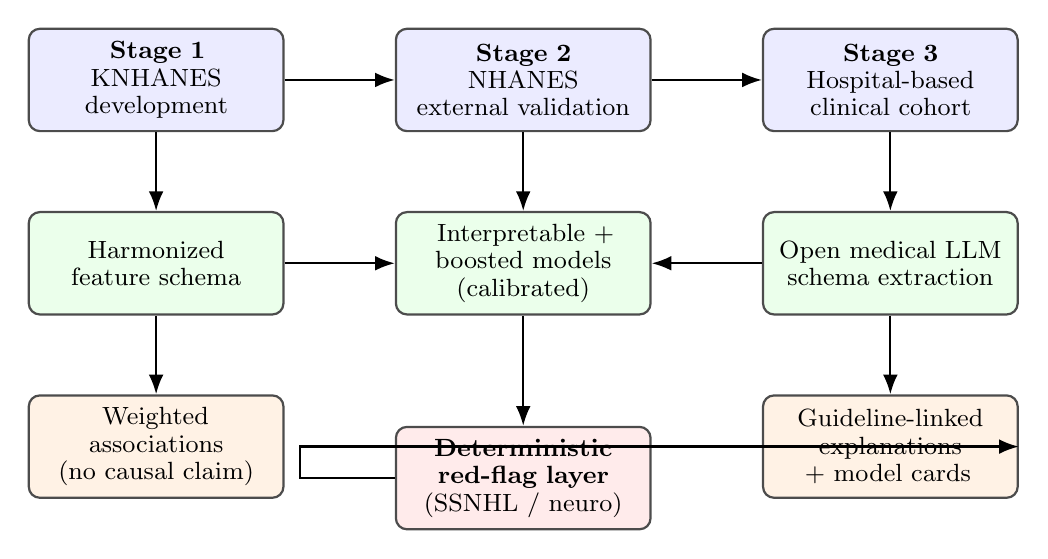
\begin{tikzpicture}[
  node distance=10mm and 14mm,
  box/.style={rectangle, rounded corners, draw=black!70, thick, align=center,
    text width=30mm, minimum height=13mm, font=\small\linespread{0.9}\selectfont},
  data/.style={box, fill=blue!8},
  ai/.style={box, fill=green!8},
  safe/.style={box, fill=red!8},
  outn/.style={box, fill=orange!10},
  arr/.style={-{Latex[length=2.5mm]}, thick}
]
\node[data] (knhanes) {\textbf{Stage 1}\\KNHANES\\development};
\node[data, right=of knhanes] (nhanes) {\textbf{Stage 2}\\NHANES\\external validation};
\node[data, right=of nhanes] (clinic) {\textbf{Stage 3}\\Hospital-based\\clinical cohort};

\node[ai, below=of knhanes] (harm) {Harmonized\\feature schema};
\node[ai, below=of nhanes] (model) {Interpretable +\\boosted models\\(calibrated)};
\node[ai, below=of clinic] (llm) {Open medical LLM\\schema extraction};

\node[safe, below=14mm of model] (redflag) {\textbf{Deterministic}\\\textbf{red-flag layer}\\(SSNHL / neuro)};

\node[outn, below=of harm] (assoc) {Weighted\\associations\\(no causal claim)};
\node[outn, below=of llm] (explain) {Guideline-linked\\explanations\\+ model cards};

\draw[arr] (knhanes) -- (nhanes);
\draw[arr] (nhanes) -- (clinic);
\draw[arr] (knhanes) -- (harm);
\draw[arr] (nhanes) -- (model);
\draw[arr] (clinic) -- (llm);
\draw[arr] (harm) -- (model);
\draw[arr] (llm) -- (model);
\draw[arr] (model) -- (redflag);
\draw[arr] (harm) -- (assoc);
\draw[arr] (llm) -- (explain);
\draw[arr] (redflag.west) -- ++(-1.2,0) |- (explain.east);
\end{tikzpicture}
\caption{STARS conceptual framework. Public survey data (blue) feed a harmonized schema and calibrated, interpretable models (green); an open medical language model performs schema-constrained extraction in the clinical extension. A deterministic red-flag safety layer (red) can override probabilistic output to force urgent referral, so a low predicted risk never suppresses time-critical SSNHL care. Outputs (orange) are associations and guideline-linked explanations, not diagnoses.}
\label{fig:framework}
\end{figure}

\begin{figure}[htbp]
\centering
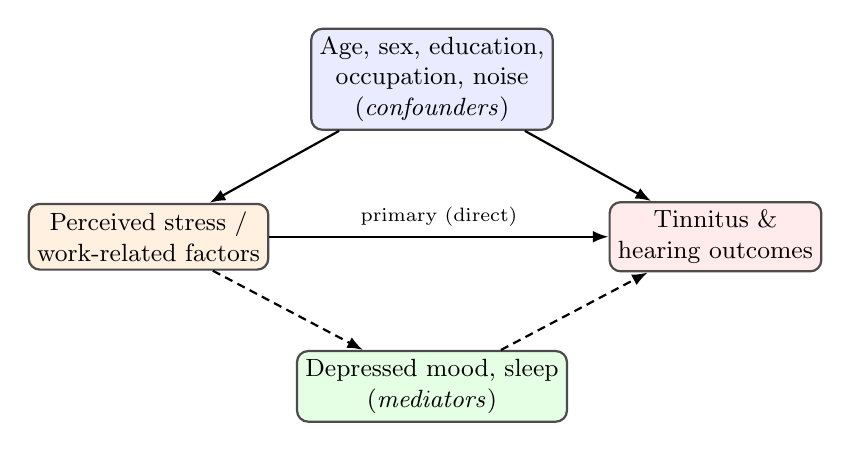
\begin{tikzpicture}[
  every node/.style={font=\small},
  var/.style={rectangle, rounded corners, draw=black!70, thick, align=center,
    inner sep=3pt, minimum height=8mm},
  conf/.style={var, fill=blue!8},
  expo/.style={var, fill=orange!12},
  med/.style={var, fill=green!10},
  outv/.style={var, fill=red!8},
  a/.style={-{Latex[length=2mm]}, thick},
  amed/.style={-{Latex[length=2mm]}, thick, densely dashed}
]
\node[expo] (stress) at (0,0) {Perceived stress /\\work-related factors};
\node[outv] (outc) at (7.2,0) {Tinnitus \&\\hearing outcomes};
\node[med] (dep) at (3.6,-1.9) {Depressed mood, sleep\\(\emph{mediators})};
\node[conf] (conf) at (3.6,2.0) {Age, sex, education,\\occupation, noise\\(\emph{confounders})};

\draw[a] (stress) -- node[above,font=\scriptsize]{primary (direct)} (outc);
\draw[amed] (stress) -- (dep);
\draw[amed] (dep) -- (outc);
\draw[a] (conf) -- (stress);
\draw[a] (conf) -- (outc);
\end{tikzpicture}
\caption{Assumed causal directed acyclic graph (DAG). The minimal sufficient adjustment set (blue confounders) is used in the \emph{primary} analysis. Depressed mood and sleep (green) are treated as \emph{mediators} of the stress$\rightarrow$outcome path (dashed); conditioning on them (extended model) is a mediator-adjusted, potentially overadjusted estimate reported separately. Restricting to employed adults can open a selection/collider path, so all-adult analysis is primary and employed-restricted analysis is secondary.}
\label{fig:dag}
\end{figure}

\begin{table}[htbp]
\centering
\caption{Selected public datasets for HEAR-WORK AI}
\label{tab:datasets}
\begin{tabular}{p{0.18\linewidth}p{0.26\linewidth}p{0.24\linewidth}p{0.22\linewidth}}
\toprule
Dataset & Role & Strengths & Main limitations \\
\midrule
KNHANES & Primary development dataset & Korean population relevance; audiometry in selected cycles; tinnitus and health variables; survey weights & Cross-sectional; stress variables may be perceived stress rather than validated occupational stress; raw data access procedures required \\
NHANES & External validation dataset & Public CDC files; audiometry and noise exposure in selected cycles; rich health covariates; geographic validation & U.S. population; cycle-specific hearing and tinnitus variables; complex survey design \\
OHHR / Zenodo audiology data & Secondary method testing & Audiology-specific measurements; useful for model benchmarking & May lack stress, occupation, or tinnitus variables \\
OpenNeuro tinnitus datasets & Optional neurophysiology substudy & Public neuroimaging or fNIRS data for tinnitus biomarkers & Not designed for occupational stress or longitudinal treatment outcomes \\
\bottomrule
\end{tabular}
\end{table}

\begin{table}[htbp]
\centering
\caption{Target harmonized variables and their availability in the primary public datasets. Availability is cycle-dependent; each derived variable records its source items and transformation in the version-controlled data dictionary.}
\label{tab:variables}
\small
\begin{tabular}{p{0.30\linewidth}p{0.14\linewidth}p{0.22\linewidth}p{0.22\linewidth}}
\toprule
Harmonized variable & Role & KNHANES & NHANES \\
\midrule
Pure-tone thresholds (per ear, per frequency) & Outcome & Selected cycles & Selected cycles \\
Tinnitus status / bother & Outcome & Selected cycles & Selected cycles \\
Self-reported hearing difficulty & Outcome (2\textsuperscript{nd}) & Yes & Yes \\
Hearing-aid use & Outcome (2\textsuperscript{nd}) & Selected cycles & Selected cycles \\
Perceived stress / depressed mood & Exposure & Yes & Yes \\
Occupation / employment status & Modifier & Yes & Yes \\
Occupational + recreational noise & Covariate & Selected cycles & Yes \\
Sleep duration & Covariate & Selected cycles & Selected cycles \\
Smoking, alcohol & Covariate & Yes & Yes \\
Cardiometabolic disease & Covariate & Yes & Yes \\
Age, sex, education & Covariate & Yes & Yes \\
Survey weight, stratum, PSU & Design & Yes & Yes \\
\bottomrule
\end{tabular}
\end{table}

\begin{table}[htbp]
\centering
\caption{Cross-national harmonization and measurement-comparability plan (excerpt). Exact cycle-specific variable codes and response categories are pinned in the repository data dictionary. Comparability governs use: \emph{low}-comparability variables are excluded from the common transportable model and entered only in country-specific extended models. ``Sel.\ cycles'' = present in selected cycles only.}
\label{tab:harmonization}
\scriptsize
\begin{tabular}{p{0.155\linewidth}p{0.145\linewidth}p{0.145\linewidth}p{0.175\linewidth}p{0.135\linewidth}p{0.085\linewidth}}
\toprule
Harmonized variable & KNHANES (source/cycle) & NHANES (source/cycle) & Original item (abridged) & Transformation rule & Compar. \\
\midrule
Tinnitus presence & Otologic Q, 2009--2012 & Audiometry Q (AUQ), sel.\ cycles & ``Ringing/noise in ears past 12 mo?'' & Any vs.\ none (binary) & High \\
Bothersome tinnitus & Otologic Q, 2009--2012 & AUQ bother item, sel.\ cycles & Annoyance / sleep / concentration & Bothersome vs.\ not & Medium \\
Pure-tone thresholds & Audiometry exam, 2010--2012 & Audiometry exam, sel.\ cycles & Air-conduction dB HL per freq. & Better/worse-ear PTA; per-ear & High \\
Perceived stress & Health Q (stress item) & DPQ / stress-related item & ``How much stress in daily life?'' & Collapse to high vs.\ low & \textbf{Low} \\
Depressed mood & PHQ-9 / mood item & PHQ-9 (DPQ) & Standardized depression items & Screen-positive vs.\ negative & Medium \\
Occupation / employment & Socioecon.\ Q & Occupation (OCQ) & Job category, employed y/n & Common category crosswalk & Medium \\
Occupational noise & Sel.\ cycles & Noise exposure (AUQ) & Loud-noise exposure, duration & Duration/intensity + binary & Medium \\
Sleep duration & Health Q & Sleep (SLQ) & Average hours of sleep & Continuous hours & Medium \\
Smoking / alcohol & Health Q & SMQ / ALQ & Current status, quantity & Standard categories & High \\
Age, sex, education & Demographics & Demographics (DEMO) & --- & Direct / crosswalk & High \\
Survey weight, stratum, PSU & Design vars & Design vars & --- & Kept for design-consistent SEs & High \\
\bottomrule
\end{tabular}
\end{table}

\begin{table}[htbp]
\centering
\caption{Intended-use specification for the two prediction models. Both are \emph{research risk-stratification} tools only; neither is a screening, diagnostic, or triage device. The specification is fixed before validation so that performance is judged against a declared purpose.}
\label{tab:intended}
\small
\begin{tabular}{p{0.24\linewidth}p{0.70\linewidth}}
\toprule
Dimension & Specification \\
\midrule
Purpose & Research risk stratification for cohort description and hypothesis generation; \emph{not} individual screening, diagnosis, triage, or treatment guidance. \\
Target user & Researchers/epidemiologists analyzing survey or, later, deidentified cohort data. \\
Prediction time & Cross-sectional (concurrent survey visit); no temporal/prognostic claim. \\
Target population & Adults 40--69 y in the fixed audiometry windows; not generalized beyond. \\
Inputs & Prespecified harmonized covariates (Table~\ref{tab:variables}); no free-text or image inputs in the public-data models. \\
Output / decision & Calibrated probability for research stratification; drives \emph{no} clinical action. \\
Cost of false positive & Low in research use; would be non-trivial if misused for screening (over-referral) --- such use is contraindicated. \\
Cost of false negative & Low in research use; dangerous if misused clinically (missed disease) --- such use is contraindicated. \\
Contraindicated uses & Individual diagnosis, treatment decisions, insurance/employment decisions, or any deployment without prospective clinical validation and regulatory review. \\
Safety interaction & The deterministic red-flag layer (Table~\ref{tab:redflag}) overrides model output for time-critical symptoms regardless of predicted probability. \\
\bottomrule
\end{tabular}
\end{table}

\begin{table}[htbp]
\centering
\caption{AI components and safety constraints}
\label{tab:ai}
\begin{tabular}{p{0.24\linewidth}p{0.34\linewidth}p{0.30\linewidth}}
\toprule
Component & Intended use & Safety constraint \\
\midrule
Survey harmonization & Map KNHANES/NHANES variables to common schema & Human-readable mapping file and version control \\
Statistical baseline & Estimate adjusted associations and transparent risk scores & Survey-aware methods; no causal claims from cross-sectional data \\
MedGemma or similar open medical LLM & Extract fixed fields from deidentified clinical notes in future cohorts & Clinician verification; no diagnosis or treatment recommendation \\
Retrieval-augmented explanation & Draft evidence-linked explanations for researchers and clinicians & Curated sources only; unsupported outputs flagged \\
Red-flag rule layer & Identify sudden hearing-loss or neurologic warning signs & Deterministic referral rules override probabilistic model \\
\bottomrule
\end{tabular}
\end{table}

\begin{table}[htbp]
\centering
\caption{Prespecified evaluation metrics (frozen before external validation). The right column shows \emph{synthetic-scaffold} values that verify pipeline wiring only: they are computed on randomly generated data, carry \textbf{no} epidemiological meaning, and must not be read as results. Real-data estimates replace them when KNHANES/NHANES files are supplied.}
\label{tab:metrics}
\small
\begin{tabular}{p{0.24\linewidth}p{0.46\linewidth}p{0.20\linewidth}}
\toprule
Dimension & Metric(s) & \textit{Synthetic scaffold (not a result)} \\
\midrule
Discrimination & AUROC, AUPRC (unweighted and survey-weighted) & Tinnitus: 0.64 / 0.49 \\
Calibration & Calibration-in-the-large and calibration slope, reported separately, before and after recalibration; Brier score; plots & Tinnitus Brier: 0.20 \\
Transportability & Common-support region; case-mix-standardized performance; reduced-common vs.\ country-specific model & Reported per target \\
Clinical utility & Decision-curve net benefit & Reported per target \\
Interpretability & SHAP importance (descriptive; caveated for correlated predictors) & Reported per target \\
Fairness & Subgroup AUROC \& calibration: sex, age, employment, noise, asymmetry, SES, race/ethnicity & Reported per subgroup \\
LLM extraction & Exact match; precision/recall/F1; omission; span agreement; temporal/laterality/onset/duration accuracy; doc-level match; run consistency; clinically significant error rate & Clinical extension \\
Safety layer & Sensitivity (95\% CI); specificity/over-referral; subgroup \& robustness (Table~\ref{tab:redflag}) & Target $\rightarrow$ 1.0 \\
\bottomrule
\end{tabular}
\end{table}

\begin{table}[htbp]
\centering
\caption{Prespecified evaluation plan for the deterministic red-flag (SSNHL/neurologic) safety layer. Sensitivity (red-flag recall) is the primary metric because a missed red flag is the costly error; but a perfect score on a finite test set does not guarantee zero real-world misses, and this limitation is stated explicitly.}
\label{tab:redflag}
\small
\begin{tabular}{p{0.28\linewidth}p{0.66\linewidth}}
\toprule
Evaluation element & Prespecification \\
\midrule
Vignette set & $\geq$200 vignettes; composition fixed: real deidentified clinical cases, expert-authored cases, and synthetic cases in a stated ratio (e.g., 40/30/30\%). \\
Reference labeling & Each vignette independently labeled by $\geq$2 otolaryngology/audiology experts; disagreements adjudicated. \\
Inter-rater agreement & Reported (Cohen's/Fleiss' $\kappa$) before adjudication. \\
Primary metric & Sensitivity (red-flag recall) with 95\% CI. \\
Secondary metrics & Specificity and over-referral rate with 95\% CIs. \\
Subgroup performance & By laterality (unilateral/bilateral), onset (acute/gradual), and vertigo/neurologic signs. \\
Robustness & Negation, ambiguous temporal expressions, and colloquial patient phrasing explicitly tested. \\
Error analysis & Every missed red flag audited and reported as a critical failure. \\
Stated limitation & Finite-set sensitivity of 1.0 is a target, not a guarantee of zero misses in deployment. \\
\bottomrule
\end{tabular}
\end{table}

\begin{thebibliography}{99}
\bibitem[Baigi et~al.(2011)]{baigi2011tinnitus} Baigi A, Oden A, Almlid-Larsen V, Barrenäs ML, Holgers KM. (2011). Tinnitus in the general population with a focus on noise and stress: A public health study. \textit{Ear and Hearing}, 32(6), 787--789. doi:10.1097/AUD.0b013e31822229bd
\bibitem[Chakrabarty et~al.(2024)]{chakrabarty2024depression} Chakrabarty S, et al. (2024). Contribution of tinnitus and hearing loss to depression: NHANES population data. \textit{Ear and Hearing}.
\bibitem[Chandrasekhar et~al.(2019)]{chandrasekhar2019ssnhl} Chandrasekhar SS, Tsai Do BS, Schwartz SR, et al. (2019). Clinical practice guideline: Sudden hearing loss (update). \textit{Otolaryngology--Head and Neck Surgery}, 161(1\_suppl), S1--S45. doi:10.1177/0194599819859885
\bibitem[Collins et~al.(2024)]{collins2024tripodai} Collins GS, Moons KGM, Dhiman P, et al. (2024). TRIPOD+AI statement: Updated guidance for reporting clinical prediction models that use regression or machine learning methods. \textit{BMJ}, 385, e078378. doi:10.1136/bmj-2023-078378
\bibitem[Google Research(2025)]{medgemma2025blog} Google Research. (2025). MedGemma: Open models for health AI development. \url{https://research.google/blog/medgemma-our-most-capable-open-models-for-health-ai-development/}
\bibitem[Google Health AI(2026)]{medgemma2026docs} Google Health AI Developer Foundations. (2026). MedGemma. \url{https://developers.google.com/health-ai-developer-foundations/medgemma}
\bibitem[Ha et~al.(2022)]{ha2022localization} Ha J, Kim H, Lee JH, Park HY. (2022). Sound localization in patients with a unilateral hearing aid: Discordance between the right and left ears. \textit{Laryngoscope Investigative Otolaryngology}, 7(2), 578--584. doi:10.1002/lio2.769
\bibitem[Hoffman et~al.(2020)]{hoffman2020noise} Hoffman HJ, et al. (2020). Noise exposure and hearing loss: Data from U.S. health surveys. CDC/NIOSH report.
\bibitem[Joo et~al.(2015)]{joo2015hrqol} Joo YH, Han K, Park KH. (2015). Association of hearing loss and tinnitus with health-related quality of life: The Korea National Health and Nutrition Examination Survey. \textit{PLoS ONE}, 10(6), e0131247.
\bibitem[Kim et~al.(2022)]{kim2022bppv} Kim H, Ha J, Lee JH, Jang JH, Park HY, Choung YH. (2022). Early management for traumatic benign paroxysmal positional vertigo in traumatically injured patients. \textit{Injury}, 53(1), 302--307. doi:10.1016/j.injury.2021.07.042
\bibitem[Kim et~al.(2021)]{kim2021ct} Kim H, Choo OS, Ha J, Jang JH, Park HY, Choung YH. (2021). A new CT parameter for predicting residual hearing preservation in cochlear implantation: The basal turn--facial ridge angle. \textit{Otology \& Neurotology}, 42(2), 204--211. doi:10.1097/MAO.0000000000002918
\bibitem[Mahboubi et~al.(2013)]{mahboubi2013noise} Mahboubi H, Zardouz S, Oliaei S, Pan D, Bazargan M, Djalilian HR. (2013). Noise-induced hearing threshold shift among U.S. adults and implications for noise-induced hearing loss. \textit{European Archives of Oto-Rhino-Laryngology}, 270, 461--467.
\bibitem[McCormack et~al.(2016)]{mccormack2016review} McCormack A, Edmondson-Jones M, Somerset S, Hall D. (2016). A systematic review of the reporting of tinnitus prevalence and severity. \textit{Hearing Research}, 337, 70--79. doi:10.1016/j.heares.2016.05.009
\bibitem[Park et~al.(2014)]{park2014tinnitus} Park KH, Lee SH, Koo JW, et al. (2014). Prevalence and associated factors of tinnitus: Data from the Korean National Health and Nutrition Examination Surveys 2009--2011. \textit{Journal of Epidemiology}, 24(5), 417--426.
\bibitem[Tunkel et~al.(2014)]{tunkel2014cpg} Tunkel DE, Bauer CA, Sun GH, et al. (2014). Clinical practice guideline: Tinnitus. \textit{Otolaryngology--Head and Neck Surgery}, 151(2\_suppl), S1--S40. doi:10.1177/0194599814545325
\bibitem[von Elm et~al.(2007)]{vonelm2007strobe} von Elm E, Altman DG, Egger M, Pocock SJ, Gøtzsche PC, Vandenbroucke JP. (2007). The Strengthening the Reporting of Observational Studies in Epidemiology (STROBE) statement. \textit{Annals of Internal Medicine}, 147(8), 573--577. doi:10.7326/0003-4819-147-8-200710160-00010
\bibitem[World Health Organization(2021)]{who2021world} World Health Organization. (2021). \textit{World Report on Hearing}. Geneva: WHO. \url{https://www.who.int/publications/i/item/9789240020481}
\end{thebibliography}

\end{document}
